% =====================================================================================================
% XRB-pilot workflow report: data acquisition, processing, analysis methods and machine learning.
% Describes the code at repository commit 666c2e0 (v1-v13). No analysis was re-run for this report.
% Compile: latexmk -pdf workflow_report.tex
% =====================================================================================================
\documentclass[11pt,a4paper]{article}
\usepackage[T1]{fontenc}
\usepackage[utf8]{inputenc}
\usepackage{lmodern}
\usepackage[margin=2.2cm]{geometry}
\usepackage{amsmath,amssymb,bm}
\usepackage{graphicx}
\usepackage{booktabs,tabularx,longtable,multirow,array}
\usepackage[table]{xcolor}
\usepackage{tikz}
\usetikzlibrary{positioning,arrows.meta,fit,calc,shapes.geometric,shapes.misc,backgrounds,decorations.pathreplacing,matrix}
\usepackage{algorithm}
\usepackage{algpseudocode}
\usepackage{enumitem}
\usepackage{microtype}
\usepackage[font=small,labelfont=bf]{caption}
\usepackage{fancyhdr}
\usepackage[round,authoryear]{natbib}
\usepackage[obeyspaces,spaces]{url}
\usepackage[colorlinks=true,linkcolor=blue!50!black,citecolor=blue!50!black,urlcolor=blue!50!black]{hyperref}
\usepackage[capitalise,noabbrev]{cleveref}
\setlist{itemsep=1.5pt,topsep=3pt}
\setlength{\emergencystretch}{3em}
\renewcommand{\topfraction}{0.85}\renewcommand{\bottomfraction}{0.7}\renewcommand{\textfraction}{0.1}
\renewcommand{\floatpagefraction}{0.75}\setcounter{topnumber}{3}\setcounter{bottomnumber}{2}\setcounter{totalnumber}{4}
\pagestyle{fancy}\fancyhf{}
\fancyfoot[L]{\footnotesize XRB-pilot workflow report (commit \texttt{666c2e0})}
\fancyfoot[R]{\footnotesize\thepage}
\renewcommand{\headrulewidth}{0pt}
\crefname{algorithm}{Algorithm}{Algorithms}

% ---------------------------------------------------------------- macros
% \code and \file: typewriter text that may break after / _ . - and at spaces (url package, verbatim-like argument)
\DeclareUrlCommand\code{\urlstyle{tt}}
\DeclareUrlCommand\file{\urlstyle{tt}}
\MakeRobust\code \MakeRobust\file
\newcommand{\vect}[1]{\bm{#1}}
\newcommand{\Xm}{\mathbf{X}}
\newcommand{\yv}{\mathbf{y}}
\newcommand{\gv}{\mathbf{g}}
\newcommand{\wv}{\mathbf{w}}
\newcommand{\indic}[1]{\mathbf{1}\!\left[#1\right]}
\newcommand{\BA}{\mathrm{BA}}
\newcommand{\AUC}{\mathrm{AUC}}
\newcommand{\sgn}{\operatorname{sgn}}
\newcommand{\median}{\operatorname{median}}
\newcommand{\sinc}{\operatorname{sinc}}

% ---------------------------------------------------------------- colours and flowchart styles (as report_en/main.tex)
\definecolor{bhblue}{HTML}{2A78D6}
\definecolor{nsorange}{HTML}{EB6834}
\definecolor{inkgrey}{HTML}{52514E}
\definecolor{boxgrey}{HTML}{F4F3EF}
\definecolor{tagprim}{HTML}{1F4E9A}
\definecolor{tagsec}{HTML}{3C6E3C}
\definecolor{tagexp}{HTML}{8A5A00}
\definecolor{tagpost}{HTML}{9B2D2D}
\definecolor{tagdesc}{HTML}{52514E}
\tikzset{
  fc/.style={rounded corners=2pt, align=center, font=\scriptsize, inner sep=2.2pt,
             execute at begin node={\hyphenpenalty=10000\exhyphenpenalty=10000\relpenalty=10000\binoppenalty=10000\relax}},
  fc data/.style={fc, rounded corners=0pt, draw=tagexp, fill=tagexp!9},
  fc proc/.style={fc, draw=tagsec, fill=tagsec!9},
  fc model/.style={fc, draw=tagprim, fill=tagprim!8},
  fc old/.style={fc, draw=inkgrey!55, dashed, fill=white, text=inkgrey},
  fc gate/.style={fc, chamfered rectangle, chamfered rectangle xsep=1.4mm, draw=inkgrey, fill=boxgrey},
  fc dec/.style={fc, diamond, aspect=2.4, draw=inkgrey, fill=white, inner sep=0.6pt},
  fc yes/.style={fc, draw=green!40!black, line width=0.6pt, fill=green!14},
  fc no/.style={fc, draw=inkgrey, fill=black!7},
  fc descr/.style={fc, draw=tagdesc, dashed, fill=white},
  fc arr/.style={-{Stealth[length=1.7mm]}, semithick, inkgrey},
  fc head/.style={font=\scriptsize\bfseries, text=inkgrey, align=center},
  fc ver/.style={draw=inkgrey, fill=inkgrey, text=white, font=\tiny\bfseries\sffamily, rounded corners=1pt, inner sep=1.1pt,
                 anchor=south west, minimum height=0pt, text width=, align=left},
  fc note/.style={font=\tiny, text=inkgrey, align=flush left, inner sep=1pt,
               execute at begin node={\hyphenpenalty=10000\exhyphenpenalty=10000\relax}},
}

\title{\textbf{XRB-pilot workflow report}\\[4pt]
\large Data acquisition, processing, data-analysis methods and machine learning\\
for black hole versus neutron star classification with RXTE, NICER and MAXI}
\author{}
\date{October 2026 \quad$\cdot$\quad describes repository \texttt{Chipwwwwww/XRB-pilot} at commit \texttt{666c2e0} (analysis rounds v1--v13)}

\begin{document}
\maketitle
\thispagestyle{fancy}

\begin{center}
\begin{minipage}{0.9\textwidth}
\small
\textbf{What this document is.} A step-by-step description of how the project works.
\begin{itemize}
\item which archives and catalogues are queried, and how files are downloaded and logged;
\item how observations are selected;
\item how spectra, light curves and event files are turned into features;
\item which machine-learning models are trained, and how;
\item how they are evaluated, and how everything is re-run.
\end{itemize}
Every rule, parameter and formula was read from the code (\file{scripts/}, \file{config.py}). Where useful, it was
cross-checked with the technical report \file{report_en/main.pdf}. The results themselves are covered in the paper draft
and the summary report; they appear here only as sample sizes.
\end{minipage}
\end{center}

\tableofcontents
\clearpage

% =====================================================================================================
\section{Overview of the workflow}\label{sec:overview}
% =====================================================================================================

\subsection{The task}
Each X-ray binary in the project is labelled from external evidence:
\begin{itemize}
\item \emph{black hole} (BH): a dynamical mass measurement;
\item \emph{neutron star} (NS): type-I X-ray bursts or pulsations.
\end{itemize}
The workflow turns single X-ray observations of these sources into feature vectors, using:
\begin{itemize}
\item RXTE/PCA spectra and light curves;
\item NICER/XTI event files;
\item MAXI/GSC daily light curves.
\end{itemize}
Classifiers are trained on the feature vectors. Their scores are always computed for sources that the model did not see
in training, and they are evaluated with statistics that treat the \emph{source}, not the observation, as the independent
unit. Everything is driven by Python scripts. HEASoft is used only where no Python equivalent exists: the XSPEC
cross-check, the HI4PI $N_\mathrm{H}$ look-up and the NICER 3C50 background.

\subsection{The workflow at a glance}
\Cref{fig:workflow} shows the whole chain, and \cref{tab:stages} lists the stages with their scripts and outputs. The
chain has five parts, each described in later sections:
\begin{enumerate}
\item \emph{External databases} (\cref{sec:acquisition}): source catalogues, observation catalogues and data archives.
\item \emph{Sample construction} (\cref{sec:samples}): which sources, and which of their observations.
\item \emph{Processing and feature extraction} (\cref{sec:rxte,sec:nicer}).
\item \emph{Data model} (\cref{sec:datamodel}): stored tables and the matrices given to the models.
\item \emph{Modelling and evaluation} (\cref{sec:ml,sec:evaluation}).
\end{enumerate}
\Cref{sec:operations} covers running, logging and reproduction.

\begin{figure}[htbp]
\centering
\begin{tikzpicture}[x=1cm, y=1cm,
  db/.style={fc data, text width=2.75cm, minimum height=17mm},
  st/.style={fc proc, text width=2.75cm, minimum height=17mm},
  md/.style={fc model, text width=2.75cm, minimum height=17mm},
  outb/.style={fc, draw=inkgrey, fill=boxgrey, text width=2.75cm, minimum height=17mm},
  lane/.style={font=\scriptsize\bfseries, text=inkgrey, anchor=east}]
  % row 1: external databases
  \node[db] (lab) at (1.55,0)  {\textbf{label catalogues}\\ BlackCAT, Marcel+2026, Galloway+2008, MINBAR, pulsar lists};
  \node[db] (pos) at (4.75,0)  {\textbf{positions}\\ CDS Sesame (SIMBAD); MINBAR source table};
  \node[db] (cat) at (7.95,0)  {\textbf{observation catalogues}\\ RXTE MissionLongData; TAP \texttt{xtemaster}, \texttt{nicermastr}};
  \node[db] (arc) at (11.15,0) {\textbf{data archives}\\ HEASARC RXTE tree; NICER AWS mirror; MAXI; GitHub};
  \node[db] (cal) at (14.35,0) {\textbf{calibration}\\ RXTE responses; NICER CALDB (3C50); HI4PI};
  % row 2: selection, retrieval, processing
  \node[st] (sel) at (1.55,-2.55)  {\textbf{select sources}\\ label rule, position match, minimum number of eligible observations};
  \node[st] (rank) at (4.75,-2.55) {\textbf{rank observations}\\ time-stratified groups, seeded order (Alg.~\ref{alg:sampling})};
  \node[st] (get) at (7.95,-2.55)  {\textbf{retrieve}\\ HTTPS download, range requests or streaming; SHA256 log};
  \node[st] (proc) at (11.15,-2.55) {\textbf{process}\\ net spectra, cospectra, colours, rms, $\nu_c$; background; bursts};
  \node[fc gate, text width=2.75cm, minimum height=17mm] (qual) at (14.35,-2.55) {\textbf{quality rules}\\ fail: try next candidate in the group};
  % row 3: data model, models, evaluation
  \node[outb] (tab) at (1.55,-5.1)  {\textbf{feature tables}\\ \file{features.npz}, \file{*_features.csv}, \file{observations.csv}};
  \node[md] (mat) at (4.75,-5.1)  {\textbf{design matrices}\\ $(\Xm,\yv,\gv)$; joins by ObsID; missing values};
  \node[md] (fit) at (7.95,-5.1)  {\textbf{models}\\ LR, RF (+ 6 others in the search); LOSO, nested or frozen};
  \node[md] (ev) at (11.15,-5.1)  {\textbf{evaluation}\\ AUC, balanced accuracy; source bootstrap; permutation tests};
  \node[outb] (res) at (14.35,-5.1) {\textbf{outputs}\\ \file{results/}, \file{figures/}, reports, decision log};
  \foreach \a/\b in {sel/rank, rank/get, get/proc, proc/qual, tab/mat, mat/fit, fit/ev, ev/res} \draw[fc arr] (\a) -- (\b);
  \draw[fc arr] (lab) -- (sel); \draw[fc arr] (pos.south) -- ++(0,-0.4) -| ([xshift=4mm]sel.north);
  \draw[fc arr] (cat) -- (rank); \draw[fc arr] (arc) -- (get); \draw[fc arr] (cal) -- (proc);
  \draw[fc arr] (qual.south) -- ++(0,-0.45) -| (tab.north);
  % side bar: configuration and provenance
  \node[fc, draw=tagprim, dashed, fill=white, text width=15.5cm, minimum height=8mm, anchor=north west] (cfg) at (0.18,-6.25)
    {\textbf{configuration and provenance (all stages):} \file{scripts/config.py} blocks selected by \code{XRB_VERSION};
     time-stamped plan \file{reports/preregistration_vN.md} before data; \file{logs/downloads.jsonl} (URL, bytes, SHA256);
     \file{reports/decision_log.md} (every change, with whether it was made after results); run scripts \file{run_vN.sh}.};
\end{tikzpicture}
\caption{End-to-end workflow. Amber: external databases; green: selection, retrieval and processing; blue: data model,
models and evaluation; grey: stored outputs; chamfered: a gate that can reject an observation. An observation that fails
the quality rules is replaced by the next ranked candidate of the same time group, so the sample is defined before any
spectrum or light curve is examined.}\label{fig:workflow}
\end{figure}

{\small\setlength{\tabcolsep}{3.5pt}
\begin{longtable}{@{}>{\raggedright\arraybackslash}p{2.6cm}>{\raggedright\arraybackslash}p{6.2cm}>{\raggedright\arraybackslash}p{3.6cm}>{\raggedright\arraybackslash}p{3.4cm}@{}}
\caption{Workflow stages, the scripts that implement them and their main outputs. Script numbers are those in
\file{scripts/}; RXTE and NICER have parallel chains.}\label{tab:stages}\\
\toprule
Stage & What happens & Scripts & Main outputs \\
\midrule\endfirsthead
\toprule Stage & What happens & Scripts & Main outputs \\ \midrule\endhead
\bottomrule\endfoot
Archive inspection & check the RXTE archive layout and file formats on two spectra & \file{01}, \file{05} & \file{reports/step2_fits_check.md} \\
Source tables & label lists to positions; match to observation catalogues & \file{03}, \file{13}, \file{20}, \file{28}, \file{35}, \file{38}, \file{41}, \file{47} & \file{data/*/sources.csv} \\
Candidate ranking & eligible observations, time-stratified groups, seeded order & \file{03}, \file{23}, \file{41}, \file{47}, \file{55}, \file{60} & \file{data/*/observation_candidates.csv} \\
Retrieval + processing (RXTE) & Standard Products, Standard-1, HEXTE, event mode; quality rules & \file{04}, \file{21}, \file{24}, \file{19}, \file{26}, \file{29}, \file{42}, \file{43} & \file{data/*/processed/features.npz}, timing tables \\
Retrieval + processing (NICER) & TAP, prefix/tail/streamed event files, features, 3C50 & \file{48}, \file{52}, \file{56}, \file{58}, \file{61}, \file{62} & \file{data/v9}--\file{v13/processed/*.csv} \\
Retrieval + processing (MAXI) & label freeze, Sesame matching, 1-day light curves, cuts; $N_\mathrm{H}$ & \file{37}, \file{38}, \file{45} & \file{data/v7c/maxi_points.csv}, \file{data/v8d/} \\
Bursts and states & Standard-1 burst detector, MINBAR match, rms state classes & \file{17}, \file{31}--\file{34}, \file{42} & \file{results/v4/burst_*}, \file{results/v7a/states.csv} \\
Data checks & integrity, response variation, XSPEC cross-check & \file{06}, \file{10} & \file{results/data_checks.md} \\
Modelling & LOSO, nested selection, frozen models & \file{07}, \file{11}, \file{16}, \file{27}, \file{30}, \file{44}, \file{49}, \file{54}, \file{57}, \file{59}, \file{63} & OOF prediction tables \\
Inference & source bootstrap, permutation tests, conformal sets & \file{09} and analysis scripts; \file{v4lib}--\file{v10lib} & \file{results/*/*bootstrap*.csv}, \file{*_nuc.csv} \\
Summaries & cross-round figures and tables & \file{15}, \file{40}, \file{46}, \file{51}, \file{64} & \file{figures/final/}, \file{results/final_*} \\
\end{longtable}}

\subsection{Analysis rounds and how a round runs}\label{sec:rounds}
The project grew in numbered rounds (v1--v14). \Cref{tab:rounds} lists them briefly. Every round from v2 on follows the
same procedure (\cref{fig:lifecycle}).

\begin{figure}[htbp]
\centering
\begin{tikzpicture}[x=1cm, y=1cm,
  st/.style={fc proc, text width=2.75cm, minimum height=15mm},
  gt/.style={fc gate, text width=2.75cm, minimum height=15mm}]
  \node[fc, draw=inkgrey, fill=white, text width=2.75cm, minimum height=15mm] (pl) at (1.55,0) {\textbf{plan}: \file{preregistration_vN.md}, written after all earlier results};
  \node[st] (cf) at (4.75,0) {\textbf{config block} in \file{config.py}, active only for \code{XRB_VERSION=vN}};
  \node[gt] (ck) at (7.95,0) {\textbf{earlier settings unchanged} (all earlier versions' values compared)};
  \node[gt] (ut) at (11.15,0) {\textbf{unit tests} \file{test_vNlib.py} on synthetic data (gates)};
  \node[fc data, text width=2.75cm, minimum height=15mm] (dl) at (14.35,0) {\textbf{selection and download} (logged)};
  \node[st] (fe) at (14.35,-2.45) {\textbf{features} with the frozen code of the round};
  \node[gt] (ic) at (11.15,-2.45) {\textbf{implementation checks} (IC): stop and report if one fails};
  \node[fc model, text width=2.75cm, minimum height=15mm] (an) at (7.95,-2.45) {\textbf{models and statistics} as pre-specified (primary, descriptive)};
  \node[fc, draw=inkgrey, fill=boxgrey, text width=2.75cm, minimum height=15mm] (rp) at (4.75,-2.45) {\textbf{results} CSV, figures, \file{report_vN_zh-TW.md}};
  \node[fc, draw=inkgrey, fill=boxgrey, text width=2.75cm, minimum height=15mm] (mg) at (1.55,-2.45) {\textbf{branch} \file{vN-analysis} merged to master (pull request)};
  \foreach \a/\b in {pl/cf, cf/ck, ck/ut, ut/dl, dl/fe, fe/ic, ic/an, an/rp, rp/mg} \draw[fc arr] (\a) -- (\b);
  \node[fc, draw=tagpost, dashed, fill=white, text width=15.4cm, minimum height=7mm, anchor=north west] at (0.17,-3.65)
    {\textbf{decision log} (\file{reports/decision_log.md}): every deviation, bug fix, added comparison or choice is recorded with
     the time and whether it was made after the round's results were seen; post hoc additions are labelled as such in reports.};
\end{tikzpicture}
\caption{Life cycle of one analysis round. The plan and the configuration are committed before the round's data are
downloaded. The implementation checks and unit tests are written before real results exist; if a check fails, the round
stops and the failure is reported rather than the rule being changed.}\label{fig:lifecycle}
\end{figure}

\begin{table}[htbp]
\centering\footnotesize
\caption{Analysis rounds (repository versions). ``Data'' is what the round added; plans are
\file{reports/preregistration_vN.md}.}\label{tab:rounds}
\begin{tabularx}{\textwidth}{@{}l >{\raggedright\arraybackslash}X >{\raggedright\arraybackslash}X@{}}
\toprule
Round & Data added & Main method added \\
\midrule
v1 & RXTE Standard-2 spectra, 8 sources & pipeline, LOSO, LR/RF on representations A and B \\
v2 & 31 sources, 456 observations; Standard-1 dead time & two-colour baseline H, source bootstrap, XSPEC check \\
v3 & 3--25\,keV grid; 14 BH candidates & nested increment tests (H+B vs H), source-level AUC \\
v4 & HEXTE; earlier gain epochs (v4b2); all 7949 epoch-5 pointings (v4b1) & 8-algorithm nested search, burst detector, source-equal weights \\
v5--v6 & Standard-1 timing features; 23 external sources & cospectral rms $T_1$--$T_3$; all-pairs estimator; $\nu_c$; permutation test; CCTLR; conformal sets \\
v7 & MINBAR; Cyg X-1, LMC X-1, LMC X-3; MAXI & rms state classes; burst matching; MAXI pipeline and reproduction of de Beurs et al. \\
v8 & GS 1354$-$64, SS 433; RXTE event mode; HI4PI & state-stratified bootstrap; high-frequency cospectra; $N_\mathrm{H}$ correction \\
v9--v10 & NICER N1 (prefix, then full files) & NICER streaming parser and features; pooled RXTE+NICER tests \\
v11 & NICER N2 (unseen observations) & frozen out-of-source prediction; Lorentzian fits \\
v12 & 3C50 background for N1+N2 & background correction and screening \\
v13 & NICER N3 (unseen observations) & everything frozen before download \\
v14 & -- & cross-round summary only \\
\bottomrule
\end{tabularx}
\end{table}

\subsection{Repository layout and conventions}\label{sec:layout}
\begin{itemize}
\item \textbf{Version switch.} Every script sets or reads the environment variable \code{XRB_VERSION}, and
\file{scripts/config.py} activates the corresponding parameter block. Later versions extend earlier blocks, and each new
block is checked not to change the values of earlier versions. \file{scripts/common.py} maps the version to the output
folders: \file{data/<v>/}, \file{results/<v>/}, \file{figures/<v>/} and \file{logs/<v>/} (v1 uses the top-level folders).
\item \textbf{Raw data.} Raw data stay out of git. RXTE products of v1--v3 and the v8 event files are in
\file{data/raw/}. Large sets live under \code{XRB_EXTERNAL_RAW} (default \file{~/xrb-pilot-data/raw}): v4b1, the NICER
prefixes and tails, the v13 cleaned files and the 3C50 spectra (\file{~/xrb-pilot-data/nicer_bkg_spectra}). The NICER
CALDB is under \file{~/xrb-pilot-data/caldb}.
\item \textbf{In git.} Everything derived is committed: source and candidate tables, every tried observation with its
status and exclusion reason, feature tables, out-of-fold predictions, result tables, figures and logs.
\item \textbf{Randomness.} The global seed is \code{SEED = 42}. Sampling seeds are offsets of it (\cref{tab:seeds}); the
bootstrap, permutations and models use it directly.
\item \textbf{Shared modules.} \file{common.py} (download and progress log), \file{spectra.py} (Standard-2 reader without
HEASoft), \file{config.py} (settings) and the version libraries \file{v3lib.py}--\file{v11lib.py}. Each version library
is tested by a \file{test_vNlib.py}.
\end{itemize}

% =====================================================================================================
\section{External databases and how the data are fetched}\label{sec:acquisition}
% =====================================================================================================

All inputs come from public services and are obtained by the scripts, with no manual downloads except the NICER CALDB
archive (\cref{sec:get-nicer}). \Cref{tab:sources} lists every external database, what is taken from it and how.
\Cref{fig:acq} shows how requests flow from the scripts to local storage and to the download log.

{\small\setlength{\tabcolsep}{3pt}
\begin{longtable}{@{}>{\raggedright\arraybackslash}p{3.2cm}>{\raggedright\arraybackslash}p{4.7cm}>{\raggedright\arraybackslash}p{4.4cm}>{\raggedright\arraybackslash}p{3.6cm}@{}}
\caption{External databases used by the workflow. ``Records'' and volumes are from \file{logs/downloads.jsonl}
(\cref{sec:provenance}).}\label{tab:sources}\\
\toprule
Database & What is taken & Access & Code \\
\midrule\endfirsthead
\toprule Database & What is taken & Access & Code \\ \midrule\endhead
\bottomrule\endfoot
\multicolumn{4}{@{}l}{\emph{Labels and positions}}\\
BlackCAT \citep{CorralSantana2016} & dynamically confirmed BHs (v1--v4); candidate list (v3c, descriptive) & names transcribed into \file{config.py}; candidates checked against the BlackCAT web pages & \file{config.py} (v2, v3c blocks) \\
\citet{Marcel2026}, Table 1 & 25 dynamically confirmed BHs (v7 onwards) & names transcribed into the scripts & \file{38_v7c2_select.py}, \file{47_v9_select.py} \\
\citet{Galloway2008} & type-I bursters, appendix A (v1--v3), Table 3 (v4b2) & names transcribed into \file{config.py} & \file{config.py}, \file{20_v4b2_select.py} \\
MINBAR DR1 \citep{Galloway2020} & burst list, observation list, source table with positions & figshare files 23201936, 24131849, 22851017 (2.5\,MB, 51.9\,MB, 0.7\,MB), MD5 checked & \file{31_v7b1_minbar.py}, \code{v7lib.load_minbar} \\
Pulsar lists & AMXPs and slow pulsars (Patruno \& Watts 2021); HMXB/LMXB catalogues of Liu et al. & names transcribed; catalogue tables from CDS (8 files) & \file{28_v6_select.py}, \file{38_v7c2_select.py} \\
CDS Sesame (SIMBAD) & RA/Dec of every named source & \code{GET https://cds.unistra.fr/cgi-bin/nph-sesame/-oI/SNV?<name>}; the \texttt{\%J} line is parsed; results cached in CSV & \code{sesame()} in \file{20}, \file{28}, \file{38} \\
\multicolumn{4}{@{}l}{\emph{Observation catalogues}}\\
RXTE MissionLongData & per-source FITS observation list: \code{OBSID}, \code{TIME}, \code{EXPOSURE}, \code{STD1RATE}, \code{RA}, \code{DEC}, \code{NPCU} & directory listing and \file{<name>.fits.gz} under \file{.../xte/data/archive/MissionLongData/} & \file{02}, \file{03}, \file{20}, \file{35}, \file{41} \\
HEASARC TAP \code{xtemaster} & RXTE pointings near a position (sources without a MissionLongData file) & ADQL cone query, HTTP POST to \file{.../xamin/vo/tap/sync} & \file{41_v8b_select.py} \\
HEASARC TAP \code{nicermastr} & NICER observations near a position: \code{obsid}, \code{time}, \code{exposure}, \code{num_fpm} & same service; one query per source, cached per source & \file{47_v9_select.py} \\
\multicolumn{4}{@{}l}{\emph{Data archives}}\\
HEASARC RXTE archive & Standard-2 Standard Products, Standard-1 light curves, event files, HEXTE products & HTTPS file tree; Python \code{urllib} (event files: \code{curl}); 46\,731 records, 5.2\,GB & \code{common.download}, \code{v8lib.download_curl} \\
HEASARC NICER (AWS open-data mirror) & cleaned (\code{_cl}) and unfiltered (\code{_ufa}) event files & \code{curl} HTTP range requests; 3\,384 records, 229.5\,GB read & \file{v9lib.py}, \file{v10lib.py}, \file{v11lib.py}, \file{v12_bkg3c50.sh} \\
MAXI/GSC & source index; 1-day light curves (2--4, 4--10, 10--20\,keV) & 13 category pages \file{http://maxi.riken.jp/top/lc_<cat>.html}; \file{http://maxi.riken.jp/star_data/<J>/<J>_g_lc_1day_all.dat} (143 files) & \file{38_v7c2_select.py} \\
GitHub (de Beurs et al.) & processed MAXI data and code of \citet{deBeurs2022} & GitHub API for the commit and file tree, then raw files at commit \texttt{488b785}; 487 files & \file{37_v7c1_repro.py} \\
\multicolumn{4}{@{}l}{\emph{Calibration}}\\
RXTE responses & \file{xp<obs>.rsp} per observation & with the Standard Products & \code{spectra.read_rsp} \\
NICER CALDB & 3C50 background libraries & \file{goodfiles_nicer_xti.tar.gz} (112\,180\,364 bytes, SHA256 recorded in the decision log) & \file{v12_bkg3c50.sh} \\
HI4PI & Galactic $N_\mathrm{H}$ at MAXI source positions & HEASoft \code{nh} with its HI4PI map & \file{v8d_heasoft.sh} \\
\end{longtable}}

\begin{figure}[htbp]
\centering
\begin{tikzpicture}[x=1cm, y=1cm,
  h/.style={fc data, text width=3.3cm, minimum height=12mm},
  m/.style={fc proc, text width=4.3cm, minimum height=12mm},
  s/.style={fc, draw=inkgrey, fill=boxgrey, text width=4.2cm, minimum height=12mm}]
  \node[fc head] at (1.75,0.9) {service};
  \node[fc head] at (7.0,0.9) {access method (code)};
  \node[fc head] at (12.75,0.9) {local result};
  \node[h] (h1) at (1.75,0)    {HEASARC RXTE file tree};
  \node[h] (h2) at (1.75,-1.6) {HEASARC TAP (xamin)};
  \node[h] (h3) at (1.75,-3.2) {NICER AWS mirror};
  \node[h] (h4) at (1.75,-4.8) {CDS Sesame; MINBAR (figshare); MAXI; GitHub};
  \node[m] (m1) at (7.0,0)    {\code{common.download}: skip if present, 3 tries, no retry on 404, write \file{.part} then rename};
  \node[m] (m2) at (7.0,-1.6) {ADQL cone query by POST, 4 tries; VOTable parsed with \code{astropy}};
  \node[m] (m3) at (7.0,-3.2) {\code{curl} HEAD, then range requests (16 or 64\,MB), 4 tries each; incremental gzip/FITS parser};
  \node[m] (m4) at (7.0,-4.8) {\code{common.download} or \code{urllib}; Sesame answers cached};
  \node[s] (s1) at (12.75,0)    {\file{data/raw/...} or \file{XRB_EXTERNAL_RAW/...}};
  \node[s] (s2) at (12.75,-1.6) {\file{data/raw/catalogs/nicer/nicermastr_<source>.csv}};
  \node[s] (s3) at (12.75,-3.2) {prefix and tail files (v9, v10) or memory only (v11, v13)};
  \node[s] (s4) at (12.75,-4.8) {\file{data/raw/minbar/}, \file{data/v7c/}, caches};
  \foreach \i in {1,2,3,4} {\draw[fc arr] (h\i) -- (m\i); \draw[fc arr] (m\i) -- (s\i);}
  \node[fc, draw=tagpost, dashed, fill=white, text width=15.2cm, minimum height=7mm, anchor=north west] at (0.1,-5.75)
    {every downloaded or streamed file: one JSON line in \file{logs/downloads.jsonl} with \code{url}, \code{path}, \code{bytes}, \code{sha256}, \code{utc} (and \code{tool})};
\end{tikzpicture}
\caption{Data acquisition. Each service is reached through one access function. Downloads are idempotent: a file that
already exists is not fetched again, and every new file is logged with its checksum.}\label{fig:acq}
\end{figure}

% -----------------------------------------------------------------------------------------------------
\subsection{Label lists and positions}\label{sec:get-labels}
Labels are attached to \emph{sources}, never to observations. The label sources are published tables, and the realised
source lists are the \file{data/*/sources.csv} files:
\begin{itemize}
\item \textbf{BHs, v1--v4:} the dynamically confirmed systems of BlackCAT Table~4, transcribed into the v2 block of
\file{config.py} with their MissionLongData catalogue names.
\item \textbf{BHs, v7 onwards:} the 25 systems of \citet{Marcel2026} Table~1, written as a list in the selection scripts.
\item \textbf{NSs:} type-I bursters of \citet{Galloway2008} (appendix A sections cited per source in \file{config.py}). From
v7 the MINBAR source table (115 bursters) is used instead; the external RXTE set adds accretion-powered pulsars.
\item \textbf{BH candidates} (BlackCAT, X-ray evidence only) are never labels. In v3c they were scored as prediction
targets, after the list had been checked against the BlackCAT web pages and frozen (\file{reports/v3c_candidate_verification.md}).
\end{itemize}

Positions come from three places, depending on the round:
\begin{itemize}
\item \textbf{v1--v3:} the median pointing in the source's RXTE catalogue.
\item \textbf{v4b2 onwards:} CDS Sesame. The script requests \code{https://cds.unistra.fr/cgi-bin/nph-sesame/-oI/SNV?<name>},
reads RA and Dec from the line starting with \texttt{\%J}, and caches the answer (\file{data/v7c/sesame_positions.csv},
\file{data/v4b2/missionlongdata_positions.csv}).
\item \textbf{NSs from v7:} the MINBAR source table (\file{minbar_sources_v2.7.fits}, columns \code{NAME}, \code{RA_OBJ},
\code{DEC_OBJ}).
\end{itemize}
The MINBAR burst table (\file{minbar.txt}, machine-readable format) supplies burst start times and durations
(\code{v7lib.load_minbar}). The three MINBAR files are downloaded from figshare; the MD5 sums of the two burst-related files
are fixed in \code{V7_MINBAR_FILES} in \file{config.py}.

% -----------------------------------------------------------------------------------------------------
\subsection{RXTE: catalogues and archive files}\label{sec:get-rxte}
\paragraph{Observation catalogues.}
The archive root is \file{https://heasarc.gsfc.nasa.gov/FTP/xte/data/archive/}. Its \file{MissionLongData/} directory
holds one FITS table per catalogued target. \file{02_catalogs.py} and \file{03_select_observations.py} download
\file{MissionLongData/<name>.fits.gz} and read extension 1 with \code{astropy}. The observation time is
\code{TIME + MJDREFI + MJDREFF} (MJD), and duplicated \code{OBSID}s are dropped. For v4b2, the whole directory listing
(291 catalogues) was downloaded and each catalogue's median pointing was matched to Sesame positions within $0.1^\circ$.
For new BHs without a catalogue file (v8b), the HEASARC TAP service is queried instead:
\begin{verbatim}
SELECT obsid, target_name, ra, dec, time, exposure FROM xtemaster
WHERE CONTAINS(POINT('ICRS',ra,dec),CIRCLE('ICRS',<ra>,<dec>,0.1))=1
\end{verbatim}
The query is sent by HTTP POST to \file{https://heasarc.gsfc.nasa.gov/xamin/vo/tap/sync} with \code{REQUEST=doQuery},
\code{LANG=ADQL}.

\paragraph{Archive layout and file names.} An ObsID \texttt{PPPPP-TT-VV-SS} lives under
\file{AO<n>/P<PPPPP>/<obsid>/}. The files used are listed below.

\begin{table}[htbp]
\centering\small
\caption{RXTE files read per observation (\texttt{o} = ObsID without hyphens).}\label{tab:rxtefiles}
\begin{tabularx}{\textwidth}{@{}>{\raggedright\arraybackslash}p{5.3cm} >{\raggedright\arraybackslash}X l@{}}
\toprule
Path below the ObsID directory & Content & Used in \\
\midrule
\file{stdprod/xp<o>_s2.pha.gz} & PCA Standard-2 total (source + background) spectrum, 129 channels & v1--v8 \\
\file{stdprod/xp<o>_b2.pha.gz} & \code{pcabackest} model background spectrum, same PCUs and GTIs & v1--v8 \\
\file{stdprod/xp<o>.rsp.gz} & response (RMF$\times$ARF) for that PCU combination, with \code{EBOUNDS} & v1--v8 \\
\file{pca/FS46_*.gz} & Standard-1: 0.125\,s counts per PCU (\code{XeCntPcu0}--\code{4}) and array rates & dead time (v2+), timing (v5+) \\
\file{pca/SE*.evt.gz} & event-mode files (\code{TIME}, \code{PCUID}) & v8c \\
\file{stdprod/xh<o>_s1.pha}, \file{_b1.pha} + RMF/ARF & HEXTE cluster-B spectra and responses & v4b3 \\
\bottomrule
\end{tabularx}
\end{table}

\paragraph{Locating the AO directory.} The AO number is not stored in the catalogue. \file{04_fetch_process.py} guesses
it from the proposal prefix (\code{5}$\to$AO5, \dots, \code{90}$\to$AO9, \code{91}$\to$AO10, \dots, \code{96}$\to$AO15). If the
guess returns HTTP 404, it tries AO4--AO16 in turn and caches the AO that worked for the proposal. (The v4b2 copy of the
script also scans AO1--AO4 for the early gain epochs.) The Standard-1 file names are taken from the HTML index of the
\file{pca/} directory (regular expression \verb|FS46_[^"]+\.gz|).

\paragraph{Download function.} \code{common.download(url, relative_path)} does the following:
\begin{enumerate}
\item returns the local file if it exists (re-runs never re-download);
\item otherwise fetches the URL with \code{urllib} (45\,s timeout), retrying up to three times with a 2\,s pause, but not
on HTTP 404;
\item writes the data to \file{<name>.part} and renames it, so an interrupted run leaves no truncated files;
\item appends a record with \code{url}, \code{path}, \code{bytes}, \code{sha256} and \code{utc} to
\file{logs/downloads.jsonl}, under a lock because downloads run in a thread pool (4 workers in
\file{04_fetch_process.py}).
\end{enumerate}
The RXTE event files of v8c (2.4\,GB) were fetched with \code{v8lib.download_curl}, which streams with \code{curl} into a
\file{.part} file and writes the same log record.

% -----------------------------------------------------------------------------------------------------
\subsection{NICER: TAP query, mirror and range requests}\label{sec:get-nicer}
\paragraph{Observation list.} For every source, \file{47_v9_select.py} queries the HEASARC TAP service:
\begin{verbatim}
SELECT obsid, name, ra, dec, time, exposure, num_fpm FROM nicermastr
WHERE CONTAINS(POINT('ICRS',ra,dec),CIRCLE('ICRS',<ra>,<dec>,0.05))=1
\end{verbatim}
The query runs with 6 parallel requests and 4 tries each. The VOTable is saved per source as
\file{data/raw/catalogs/nicer/nicermastr_<source>.csv}. The later rounds (v11, v13) select from these cached tables, so
all three NICER observation sets come from the same catalogue snapshot.

\paragraph{File location.} Cleaned event files are read from HEASARC's AWS open-data mirror, which is byte-identical to
the HEASARC site (checked on the first 4\,MB) and about ten times faster from the analysis machine:
\begin{center}
\file{https://nasa-heasarc.s3.amazonaws.com/nicer/data/obs/<YYYY_MM>/<obsid>/xti/event_cl/ni<obsid>_0mpu7_cl.evt.gz}
\end{center}
\code{YYYY_MM} is the month of the catalogue start time. If the file is not found (HTTP 403 or 404 on the mirror), the
previous and next months are tried. The unfiltered file \file{..._0mpu7_ufa.evt.gz} is fetched only for the 3C50
background (\cref{sec:3c50}).

\paragraph{Range requests and the streaming parser.} The files are gzip-compressed FITS tables of up to several GB, so
they are never downloaded blindly:
\begin{enumerate}
\item A HEAD request (\code{curl -I}) checks that the file exists and gives its size.
\item The file is fetched in HTTP range requests (\code{curl -r a-b}; options \code{--connect-timeout 30},
\code{--speed-limit 20000}, \code{--speed-time 60}), each with up to 4 tries and a 5\,s pause.
\item Each piece is passed to an incremental parser (\code{v9lib.PrefixParser}). The parser decompresses the gzip stream
with \code{zlib}, reads the primary and \code{EVENTS} headers from 2880-byte blocks, and converts complete binary-table
rows to arrays of \code{TIME}, \code{PI} and \code{DET_ID} using a numpy dtype built from the \code{TFORMn} keywords.
\end{enumerate}
No HEASoft is needed to read the events. The three reading modes are listed in \cref{tab:nicermodes}. Parsing was checked
to agree with \code{astropy} and across the modes (implementation checks of v9--v11).

\begin{table}[htbp]
\centering\small
\caption{NICER reading modes.}\label{tab:nicermodes}
\begin{tabularx}{\textwidth}{@{}>{\raggedright\arraybackslash}p{1.9cm} >{\raggedright\arraybackslash}p{3.1cm} >{\raggedright\arraybackslash}p{1.9cm} >{\raggedright\arraybackslash}X >{\raggedright\arraybackslash}X@{}}
\toprule
Round & Function & Request size & Stop rule & Storage \\
\midrule
v9 (prefix) & \code{v9lib.stream_prefix} & 16\,MB & $\ge6$ gap-free 128\,s segments, end of file, or 300\,MB & compressed prefix + JSON metadata in \file{XRB_EXTERNAL_RAW/nicer/<obsid>/} \\
v10 (tail) & \code{v10lib.download_tail} & 64\,MB & end of file or 1\,GB compressed & tail in \file{nicer_tail/<obsid>/}; prefix + tail parsed as one stream \\
v11, v13 (stream) & \code{v11lib.stream_events} & 64\,MB, 6 in parallel & end of file or 1\,GB & nothing stored (SHA256 of the bytes read is logged); v13 keeps cleaned files of faint observations for one check \\
\bottomrule
\end{tabularx}
\end{table}

\paragraph{3C50 inputs and the CALDB.} For the background model, the script \file{v12_bkg3c50.sh} runs inside WSL Ubuntu
with HEASoft 6.37.1. It:
\begin{enumerate}
\item downloads the cleaned and unfiltered event files with \code{curl} (3 tries) and prints their SHA256 and size, which
the Python driver writes to the download log;
\item unzips them and runs \code{nibackgen3C50} (\cref{sec:3c50});
\item keeps only the resulting total and background spectra (\file{tot_<obsid>.pi}, \file{bkg_<obsid>.pi});
\item deletes the event files.
\end{enumerate}
The NICER CALDB (\file{goodfiles_nicer_xti.tar.gz} with \file{caldb.config} and \file{alias_config.fits}) was downloaded
once before the v12 data and unpacked under \file{~/xrb-pilot-data/caldb}; its size and SHA256 are in the decision log.

% -----------------------------------------------------------------------------------------------------
\subsection{MAXI, published code and absorption}\label{sec:get-maxi}
\begin{itemize}
\item \textbf{MAXI matching.} The label lists are frozen first. The MAXI source index is read from the 13 category pages
(\file{http://maxi.riken.jp/top/lc_<cat>.html}). MAXI names are resolved with Sesame and matched to the label sources within
$0.1^\circ$, with a $0.3^\circ$ fallback to the position encoded in the MAXI J-name. MAXI sources whose name contains
``with'' (blends) are excluded, as are ambiguous matches (\cref{sec:maxi}).
\item \textbf{MAXI light curves.} The 1-day light curves are downloaded from
\file{http://maxi.riken.jp/star_data/<J>/<J>_g_lc_1day_all.dat} with \code{common.download}.
\item \textbf{Published code.} For the reproduction of \citet{deBeurs2022}, \file{37_v7c1_repro.py} asks the GitHub API
for the current commit and file tree of \file{zdebeurs/3ML_methods_for_XRB_classification}. It then downloads every file
from \file{raw.githubusercontent.com} at that commit (\texttt{488b785}).
\item \textbf{Absorption.} For the absorption correction, \file{v8d_heasoft.sh} runs HEASoft \code{nh} (HI4PI, average
within $0.1^\circ$) at each MAXI source position. It also runs XSPEC to tabulate \code{tbabs}$\times$power-law
transmissions (\cref{sec:maxi}).
\end{itemize}

% -----------------------------------------------------------------------------------------------------
\subsection{Provenance log and verification}\label{sec:provenance}
\file{logs/downloads.jsonl} has one JSON object per downloaded or streamed file. Its fields are \code{url}, \code{path}
(or a note such as ``deleted after 3C50''), \code{bytes}, \code{sha256} and \code{utc}; the NICER functions add
\code{tool}, \code{file_bytes}, \code{stop}, \code{rows} and offsets. At commit \texttt{666c2e0} it holds 50\,773 records
(\cref{tab:dlsummary}). Every input can be verified byte for byte after re-download. This was done once in full: on a
second machine (macOS), the 2\,689 v1--v2 raw files were re-downloaded from the logged URLs and all SHA256 values matched.
The rebuilt \file{features.npz} agreed with the original to $\le10^{-16}$.

\begin{table}[htbp]
\centering\small
\caption{Download log by host (\file{logs/downloads.jsonl}, commit \texttt{666c2e0}). Streamed NICER records count the
bytes read, although the bytes were not stored.}\label{tab:dlsummary}
\begin{tabularx}{\textwidth}{@{}l r r >{\raggedright\arraybackslash}X@{}}
\toprule
Host & Records & Volume & Tool(s) \\
\midrule
\file{heasarc.gsfc.nasa.gov} & 46\,731 & 5.2\,GB & \code{urllib} (\code{common.download}); \code{curl} for event files \\
\file{nasa-heasarc.s3.amazonaws.com} & 3\,384 & 229.5\,GB & \code{curl} range requests (prefix, tail, stream); \code{curl} in WSL (3C50) \\
\file{raw.githubusercontent.com} & 487 & 0.01\,GB & \code{urllib} \\
\file{maxi.riken.jp} & 156 & 0.06\,GB & \code{urllib} \\
\file{cdsarc.cds.unistra.fr} & 8 & $<0.01$\,GB & \code{urllib} \\
\file{arxiv.org} & 4 & $<0.01$\,GB & \code{urllib} \\
\file{ndownloader.figshare.com} & 3 & 0.06\,GB & \code{urllib} \\
\midrule
total & 50\,773 & 234.8\,GB & \\
\bottomrule
\end{tabularx}
\end{table}

% =====================================================================================================
\section{Sample construction: sources and observations}\label{sec:samples}
% =====================================================================================================

Sample construction runs in two stages. First, \emph{sources} are chosen and labelled from published tables. Second, for each
source, \emph{observations} are chosen from the archive catalogue by a rule that uses only times, exposures, count rates and
positions, never the spectrum or the light curve. Data are downloaded and processed only after both lists are written. The
processing can reject an observation (quality rules); the next candidate of the same time group then takes its place.
\Cref{fig:selectflow} summarises the procedure.

\begin{figure}[htbp]
\centering
% Source labelling, eligibility and time-stratified sampling (Algorithm 1). Copied from report_en/figures/flowcharts (styles in workflow_report.tex).
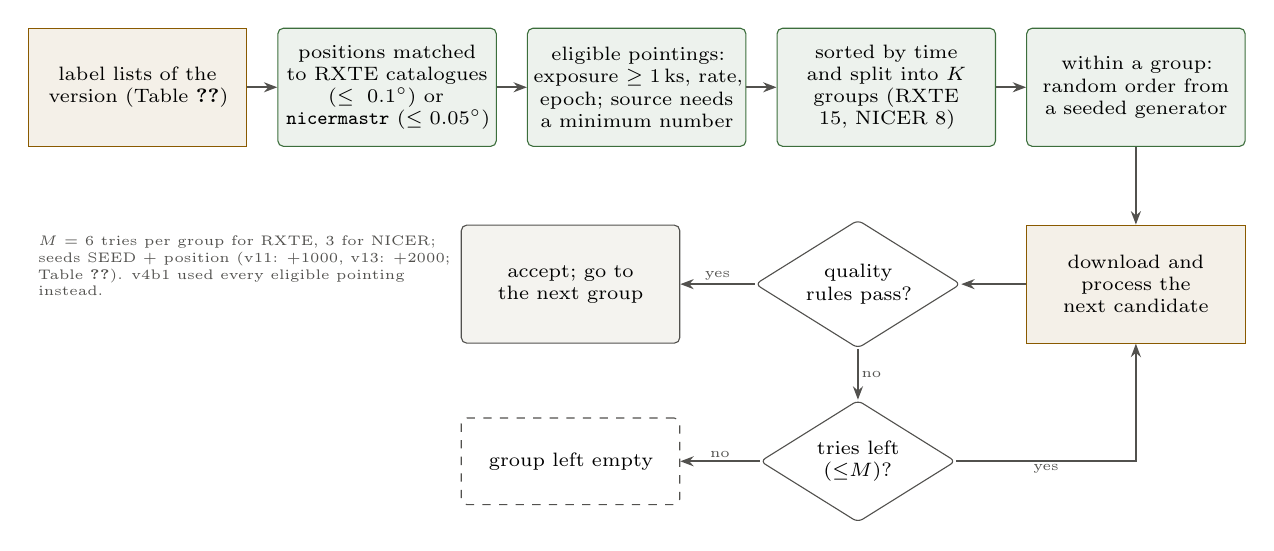
\begin{tikzpicture}[x=1cm, y=1cm,
  st/.style={fc proc, text width=2.62cm, minimum height=15mm},
  lab/.style={font=\tiny, text=inkgrey, inner sep=1pt}]
  % row 1: sources and eligible pointings
  \node[fc data, text width=2.62cm, minimum height=15mm] (lb) at (1.45,0) {label lists of the version (Table~\ref{tab:labelrules})};
  \node[st] (mt) at (4.62,0) {positions matched to RXTE catalogues ($\le0.1^\circ$) or \texttt{nicermastr} ($\le0.05^\circ$)};
  \node[st] (el) at (7.79,0) {eligible pointings: exposure $\ge1$\,ks, rate, epoch; source needs a minimum number};
  \node[st] (gr) at (10.96,0) {sorted by time and split into $K$ groups (RXTE 15, NICER 8)};
  \node[st] (rk) at (14.13,0) {within a group: random order from a seeded generator};
  \foreach \a/\b in {lb/mt,mt/el,el/gr,gr/rk} \draw[fc arr] (\a) -- (\b);
  % row 2: the try-and-accept loop (right to left)
  \node[fc data, text width=2.62cm, minimum height=15mm] (dl) at (14.13,-2.5) {download and process the next candidate};
  \node[fc dec, text width=1.7cm, aspect=1.6] (q) at (10.6,-2.5) {quality rules pass?};
  \node[fc, draw=inkgrey, fill=boxgrey, text width=2.62cm, minimum height=15mm] (ok) at (6.95,-2.5) {accept; go to the next group};
  \node[fc dec, text width=1.55cm, aspect=1.6] (mx) at (10.6,-4.75) {tries left (${\le}M$)?};
  \node[fc, draw=inkgrey, fill=white, dashed, text width=2.62cm, minimum height=11mm] (gv) at (6.95,-4.75) {group left empty};
  \draw[fc arr] (rk) -- (dl);
  \draw[fc arr] (dl) -- (q);
  \draw[fc arr] (q) -- node[lab, above] {yes} (ok);
  \draw[fc arr] (q) -- node[lab, right] {no} (mx);
  \draw[fc arr] (mx.east) -| node[lab, pos=0.25, below] {yes} (dl.south);
  \draw[fc arr] (mx) -- node[lab, above] {no} (gv);
  \node[fc note, text width=5.2cm, anchor=north west] at (0.15,-1.85)
     {$M$ = 6 tries per group for RXTE, 3 for NICER; seeds \code{SEED + position} (v11: $+1000$, v13: $+2000$; Table~\ref{tab:seeds}). v4b1 used every eligible pointing instead.};
\end{tikzpicture}

\caption{Selection of sources and observations. Apart from the quality rules, the choice of an observation depends only on
the label list, the catalogue position, the eligibility rules, the time order and a seeded random order.}\label{fig:selectflow}
\end{figure}

% -----------------------------------------------------------------------------------------------------
\subsection{Source labels}\label{sec:labels}
The label is a property of the source: $y=1$ for a black hole and $y=0$ for a neutron star. A BH needs a dynamical mass
function, and an NS needs type-I X-ray bursts or coherent accretion-powered pulsations. BH candidates (X-ray evidence only)
are never labels. \Cref{tab:labelrules} lists the rule of each round. The realised source lists, with the evidence and a
reference URL for every source, are \file{data/<v>/sources.csv}.

\begin{table}[htbp]
\centering\small
\caption{Labelling and eligibility rules by round. ``Pointing'' is the largest separation allowed between an observation's
pointing and the source position. Every round also requires a catalogue exposure $\ge1000$\,s (RXTE: and
\code{STD1RATE}~$\ge5$\,c\,s$^{-1}$\,PCU$^{-1}$).}\label{tab:labelrules}
\begin{tabularx}{\textwidth}{@{}>{\raggedright\arraybackslash}p{1.35cm}>{\raggedright\arraybackslash}X>{\raggedright\arraybackslash}X>{\raggedright\arraybackslash}p{3.9cm}@{}}
\toprule
Round & BH rule & NS rule & Pointing; time window; minimum eligible \\
\midrule
v1 & 4 BlackCAT dynamical BHs & 4 Galloway+2008 bursters & $0.1^\circ$ from the catalogue median; gain epoch 5 to MJD 54094; 30 \\
v2, v3 & every BlackCAT Table~4 BH with a MissionLongData catalogue & every Galloway+2008 appendix-A burster with a catalogue & $0.1^\circ$; gain epoch 5 (MJD 51677--55931); 10 \\
v3c & 16 BlackCAT candidates (prediction targets only) & -- & as v2 \\
v4b2 & BlackCAT BHs found by position & Galloway+2008 Table~3 bursters found by position & $0.1^\circ$ from Sesame; all gain epochs; 10 \\
v6 & HMXB BHs (Cyg X-1, LMC X-3) & accreting millisecond pulsars; 4 slow pulsars as a stress set & as v4b2 \\
v7b2 & Cyg X-1, LMC X-1, LMC X-3 \citep{Marcel2026} & -- & $0.1^\circ$ from Sesame; gain epoch 5; 10 \\
v7c (MAXI) & \citet{Marcel2026} Table~1 & MINBAR bursters without pulsations; pulsars as a separate class & MAXI source within $0.1^\circ$ ($0.3^\circ$ fallback); $\ge100$ daily points \\
v8b & Marcel+2026 BHs not used before (GS 1354$-$64, SS 433) & -- & $0.1^\circ$ from Sesame; all gain epochs; 3 \\
v9--v13 (NICER) & Marcel+2026 Table~1, Sesame positions & MINBAR bursters; entries with another MINBAR entry within $0.05^\circ$ removed & target within $0.05^\circ$; mission; 5 \\
\bottomrule
\end{tabularx}
\end{table}

\paragraph{Confused fields.} NICER does not image, so a MINBAR source with another MINBAR source within $0.05^\circ$ is
flagged \code{excluded_confused} and not used. Nine of the 115 MINBAR sources are removed this way in \file{47_v9_select.py}.
For RXTE, the $0.1^\circ$ pointing rule plays the same role; \file{config.py} notes, for example, that 4U 1907+097 lies
about $0.4^\circ$ from the candidate XTE J1908+094.

% -----------------------------------------------------------------------------------------------------
\subsection{Catalogue-level eligibility}\label{sec:eligibility}
For RXTE (\file{03_select_observations.py} and its copies), each source's MissionLongData catalogue goes through the steps
below. The number of rows left after each step is written to \file{results/<v>/attrition_catalog.csv}:
\begin{enumerate}
\item drop duplicated \code{OBSID}s;
\item keep the time window of the round: gain epoch 5 (MJD 51677 to 54094 in v1, to 55931 from v2), or all gain epochs
(v4b2, v6, v8b);
\item keep \code{EXPOSURE}~$\ge1000$\,s;
\item keep \code{STD1RATE}~$\ge5$\,c\,s$^{-1}$\,PCU$^{-1}$;
\item keep pointings within $0.1^\circ$ of the source position (great-circle distance);
\item drop the source if fewer than the minimum number of pointings remain (\cref{tab:labelrules}). The source stays in
\file{sources.csv} with \code{included = False}.
\end{enumerate}
For NICER (\file{47_v9_select.py}), the TAP query already restricts the target position to $0.05^\circ$. The remaining
steps are: drop rows without a time, drop duplicated ObsIDs, keep \code{exposure}~$\ge1000$\,s, and require at least 5
eligible observations and a non-confused field.

% -----------------------------------------------------------------------------------------------------
\subsection{Time-stratified ranking}\label{sec:ranking}
The eligible observations of a source are sorted by time and split into $K$ consecutive groups of nearly equal size
(\code{numpy.array_split}): $K=15$ for RXTE, 8 for NICER. A seeded generator puts the observations of each group in a
random order (\cref{alg:sampling}). The seed is \code{SEED} plus an offset plus the 1-based position of the source in the
source list (\cref{tab:seeds}). The result is \file{data/<v>/observation_candidates.csv}, with one row per eligible
observation, its group (\code{time_bin}) and its rank in the group (\code{rank_in_bin}). This file is written before any
data file is downloaded.

The stratification spreads each source's sample over its history, across outbursts and states. Because the order is
random within a group, the choice does not depend on the data. If a source has fewer eligible observations than groups,
some groups are empty and every observation is a candidate.

\begin{algorithm}[htbp]
\caption{Time-stratified ranking and acceptance. RXTE: \file{03_select_observations.py} with
\file{04_fetch_process.py}; NICER: \file{47}/\file{55}/\file{60} with \file{48}/\file{52}/\file{56}/\file{61}.}\label{alg:sampling}
\begin{algorithmic}[1]
\Require eligible observations $\{(o_i,t_i)\}$ of one source; number of groups $K$; seed $\sigma$; tries per group $M$
\State sort by $t_i$ and split the index list into $K$ consecutive groups $G_1,\dots,G_K$
\State $\mathrm{rng}\gets\mathrm{default\_rng}(\sigma)$
\For{$b=1,\dots,K$}
  \State $\pi\gets\mathrm{rng.permutation}(G_b)$ \Comment{rank within the group; written to the candidate table}
\EndFor
\Statex \textit{--- later, in the fetch script, for each group independently ---}
\For{$r=1,\dots,\min(M,|G_b|)$}
  \State download and process $o_{\pi_r}$; record status and reason
  \If{every quality rule passes} accept $o_{\pi_r}$; \textbf{break} \EndIf
\EndFor
\end{algorithmic}
\end{algorithm}

\begin{table}[htbp]
\centering\small
\caption{Sampling parameters. ``Position'' is the 1-based position of the source in the list processed by the script
(for NICER, \file{data/v9/sources.csv}, counting excluded sources too). \code{SEED = 42}.}\label{tab:seeds}
\begin{tabular}{@{}l l l l@{}}
\toprule
Sample & Groups $K$ & Seed $\sigma$ & Tries per group $M$ \\
\midrule
RXTE v1, v2, v3c, v7b2, v8b & 15 & \code{SEED + position} & 6 \\
RXTE v4b2 (new sources) & 15 & \code{SEED + 100 + i} & 6 \\
RXTE v4b1 & all eligible & -- & 1 \\
NICER v9 (N1) & 8 & \code{SEED + position} & 3 \\
NICER v11 (N2) & 8 & \code{SEED + 1000 + position} & 3 \\
NICER v13 (N3) & 8 & \code{SEED + 2000 + position} & 3 \\
\bottomrule
\end{tabular}
\end{table}

% -----------------------------------------------------------------------------------------------------
\subsection{Acceptance loop and quality rules}\label{sec:quality}
The fetch scripts work through the (source, group) pairs in parallel: 4 threads for RXTE; for NICER, 8 threads in v9 and
2 in v11 and v13. Within a pair the candidates are tried in rank order. Every tried candidate becomes one row of
\file{data/<v>/observations.csv}, with its status, its reason, the download URL and the quality quantities. Rejected
observations are therefore documented, not lost.

\begin{table}[htbp]
\centering\small
\caption{Post-download quality rules. An observation is accepted only if no rule fires. ``Reason'' is the string written
to \file{observations.csv}.}\label{tab:qualityrules}
\begin{tabularx}{\textwidth}{@{}l l >{\raggedright\arraybackslash}X@{}}
\toprule
Data & Reason & Rule \\
\midrule
RXTE PCA & \code{fetch_or_read_error} & a file is missing in every AO directory, or cannot be read \\
 & \code{nonfinite} & a rebinned rate or error is not finite \\
 & \code{short_exposure} & Standard-2 \code{EXPOSURE}~$<1000$\,s \\
 & \code{low_snr} & net 5--25\,keV rate / its error $<10$ (\cref{eq:F}) \\
 & \code{high_deadtime} & dead-time fraction $>0.10$ (\cref{eq:dtf}) \\
 & \code{coord_mismatch} & header pointing $>0.1^\circ$ from the source position \\
 & \code{nonstandard_channels} & spectrum or response does not have 129 channels \\
 & \code{ebounds_coverage} & the response's energy range does not cover the common grid \\
\midrule
NICER XTI & \code{error: ...} & download or parsing error (after retries) \\
 & \code{missing (event file not found)} & no file in the catalogue month or the months before and after \\
 & \code{missing (< 3 valid segments)} & fewer than 3 usable 128\,s segments (\cref{sec:nicer}) \\
 & \code{excluded (2-10 keV rate x < 20.0)} & mean 2--10\,keV rate in the valid segments $<20$\,c\,s$^{-1}$ \\
\bottomrule
\end{tabularx}
\end{table}

Two further screens act after acceptance and do not trigger a replacement. Type-I bursts are flagged, or the affected
segments removed (\cref{sec:bursts}). From v12, NICER observations are screened on their 3C50 background fraction
(\cref{sec:3c50}).

% -----------------------------------------------------------------------------------------------------
\subsection{Disjoint NICER observation sets}\label{sec:disjoint}
NICER was used three times, each time with observations that had never been tried before:
\begin{itemize}
\item \textbf{N1} (v9, re-read in full in v10): the first time-stratified sample of the v9 sources.
\item \textbf{N2} (v11): for each included v9 source, the eligible observations \emph{not} among the 792 v9 tries, ranked
with \code{SEED + 1000 + position}. Sources not included in v9 but with 1--4 eligible observations and a non-confused field
contribute every eligible observation, one per group.
\item \textbf{N3} (v13): eligible observations of the included v9 sources that are among neither the 792 v9 tries nor the
588 v11 tries, ranked with \code{SEED + 2000 + position}.
\end{itemize}
The selection scripts compute the overlap with the earlier tries and stop with exit code 3 if it is not empty (check IC3 in
v11). All three sets come from the same cached \code{nicermastr} tables, so no new catalogue query can change the
candidates.

% -----------------------------------------------------------------------------------------------------
\subsection{Resulting samples}\label{sec:samplesizes}
\Cref{tab:samples} lists the samples that enter models or tests. Counts are recomputed from the committed
\file{observations.csv} and processed tables.

{\small\setlength{\tabcolsep}{3.5pt}
\begin{longtable}{@{}>{\raggedright\arraybackslash}p{2.9cm} >{\raggedright\arraybackslash}p{2.8cm} r r >{\raggedright\arraybackslash}p{2.1cm} >{\raggedright\arraybackslash}p{4.3cm}@{}}
\caption{Samples. ``Tried'' counts every downloaded candidate; ``Obs.'' counts the accepted (or kept) observations;
``Sources'' gives the total and the BH/NS split.}\label{tab:samples}\\
\toprule
Sample & Round, instrument & Tried & Obs. & Sources & Use \\
\midrule\endfirsthead
\toprule Sample & Round, instrument & Tried & Obs. & Sources & Use \\ \midrule\endhead
\bottomrule\endfoot
pilot & v1, PCA & 120 & 120 & 8 (4/4) & pipeline test \\
S1 (development) & v2, PCA, epoch 5 & 462 & 456 & 31 (7/24) & training and LOSO in v2--v8, v10 \\
BH candidates & v3c, PCA & 210 & 210 & 14 (14/0) & prediction only \\
S3 (all pointings) & v4b1, PCA, epoch 5 & 7\,975 & 7\,949 & 31 (7/24) & observation-budget checks \\
v4b2 sources & v4b2, PCA, all epochs & 221 & 221 & 15 (2/13) & S2 = S1 $\cup$ v4b2 (46 sources, 677 obs.) \\
E\textsubscript{new} + stress & v6, PCA, all epochs & 180 & 180 & 12 (2/10) & 8 new sources (120 obs.); 4 slow pulsars (60 obs.) \\
E (external) & v6 & -- & 341 & 23 (4/19) & frozen-model test \\
persistent BHs & v7b2, PCA, epoch 5 & 45 & 45 & 3 (3/0) & Cyg X-1, LMC X-1, LMC X-3 \\
new BHs & v8b, PCA, all epochs & 26 & 23 & 2 (2/0) & GS 1354$-$64, SS 433 \\
X (external) & v8b & -- & 379 & 26 (7/19) & frozen-model test; 99 hard-like obs.\ (5/15 sources) \\
MAXI & v7c2, GSC & -- & 132\,057 & 100: 13 BH, 48 NPNS, 39 PSR & daily points (not observations); point-level classifiers \\
N1 & v9 (prefix), XTI & 792 & 368 & 63 (9/54) & first NICER sample \\
N1 full files & v10, XTI & 368 & 366 & 63 (9/54) & N1 re-read to 1\,GB \\
N2 & v11, XTI & 588 & 318 & 60 (9/51) & unseen observations \\
N1+N2, 3C50 & v12, XTI & -- & 534 & 58 (9/49) & corrected and screened; frozen training set for v13 \\
N3 & v13, XTI & 412 & 238 & 37 (8/29) & unseen observations \\
N3, 3C50 & v13, XTI & -- & 198 & 35 (8/27) & corrected and screened test set \\
\end{longtable}}

% =====================================================================================================
\section{RXTE processing and feature extraction}\label{sec:rxte}
% =====================================================================================================

RXTE gives three kinds of input from the Proportional Counter Array (PCA; \citealt{Jahoda2006}): Standard-2 spectra, PCA Standard-1 light curves and, for one test, PCA event files
(HEXTE spectra are a fourth, minor input). Spectra are read and background-subtracted in Python
(\file{spectra.py}); HEASoft is used only for an independent check. \Cref{fig:specflow} shows the spectral chain and
\cref{fig:timingflow} the timing chain.

\begin{figure}[htbp]
\centering
% RXTE/PCA Standard-2 spectral pipeline and the representations added by each version. Copied from report_en/figures/flowcharts (styles in workflow_report.tex).
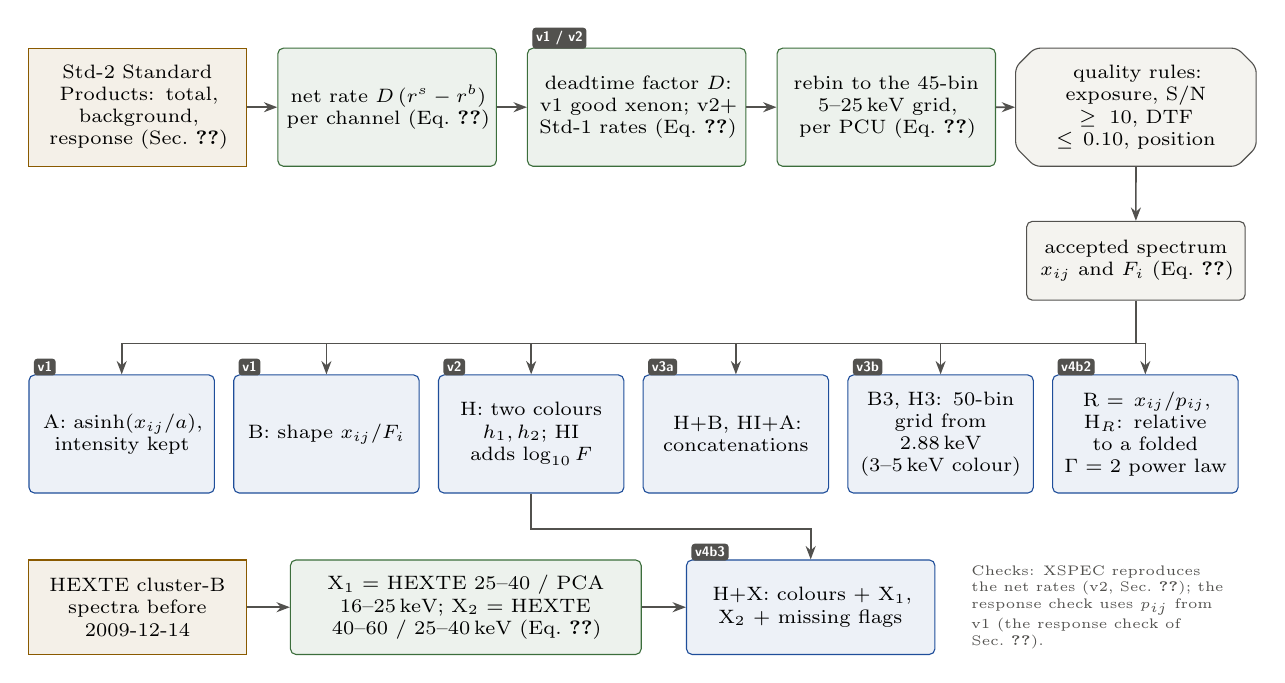
\begin{tikzpicture}[x=1cm, y=1cm,
  st/.style={fc proc, text width=2.62cm, minimum height=15mm},
  rep/.style={fc model, text width=2.2cm, minimum height=15mm},
  badge/.style={fc ver, anchor=south west}]
  % row 1: from the archive files to the rebinned spectrum
  \node[fc data, text width=2.62cm, minimum height=15mm] (f) at (1.45,0) {Std-2 Standard Products: total, background, response (Sec.~\ref{sec:pca})};
  \node[st] (net) at (4.62,0)  {net rate $D\,(r^s-r^b)$ per channel (Eq.~\ref{eq:net})};
  \node[st] (dtf) at (7.79,0)  {deadtime factor $D$: v1 good xenon; v2+ Std-1 rates (Eq.~\ref{eq:dtf})};
  \node[st] (reb) at (10.96,0) {rebin to the 45-bin 5--25\,keV grid, per PCU (Eq.~\ref{eq:rebin})};
  \node[fc gate, text width=2.62cm, minimum height=15mm] (qual) at (14.13,0) {quality rules: exposure, S/N $\ge10$, DTF $\le0.10$, position};
  \foreach \a/\b in {f/net,net/dtf,dtf/reb,reb/qual} \draw[fc arr] (\a) -- (\b);
  \node[badge] at ([xshift=2pt, yshift=-0.4pt]dtf.north west) {v1 / v2};
  % the accepted spectrum that every representation starts from
  \node[fc, draw=inkgrey, fill=boxgrey, text width=2.62cm, minimum height=10mm] (x) at (14.13,-1.95) {accepted spectrum $x_{ij}$ and $F_i$ (Eq.~\ref{eq:F})};
  \draw[fc arr] (qual) -- (x);
  % representations, each with the version that added it, fed by one bus line
  \node[rep] (A)  at (1.25,-4.15)  {A: asinh$(x_{ij}/a)$, intensity kept};
  \node[rep] (B)  at (3.85,-4.15)  {B: shape $x_{ij}/F_i$};
  \node[rep] (H)  at (6.45,-4.15)  {H: two colours $h_1,h_2$; HI adds $\log_{10}F$};
  \node[rep] (HB) at (9.05,-4.15)  {H+B, HI+A: concatenations};
  \node[rep] (B3) at (11.65,-4.15) {B3, H3: 50-bin grid from 2.88\,keV (3--5\,keV colour)};
  \node[rep] (R)  at (14.25,-4.15) {R $=x_{ij}/p_{ij}$, H$_R$: relative to a folded $\Gamma=2$ power law};
  \foreach \n/\v in {A/v1, B/v1, H/v2, HB/v3a, B3/v3b, R/v4b2} \node[badge] at ([xshift=2pt, yshift=-0.4pt]\n.north west) {\v};
  \coordinate (bus) at (0,-3.0);
  \draw[semithick, inkgrey] (x.south) -- (x.south |- bus);
  \draw[semithick, inkgrey] (A.north |- bus) -- (R.north |- bus);
  \foreach \n in {A,B,H,HB,B3,R} \draw[fc arr] (\n.north |- bus) -- (\n.north);
  % HEXTE branch (v4b3)
  \node[fc data, text width=2.62cm, minimum height=12mm] (hx) at (1.45,-6.35) {HEXTE cluster-B spectra before 2009-12-14};
  \node[fc proc, text width=4.3cm, minimum height=12mm] (hxc) at (5.62,-6.35) {X$_1$ = HEXTE 25--40 / PCA 16--25\,keV; X$_2$ = HEXTE 40--60 / 25--40\,keV (Eq.~\ref{eq:hexte})};
  \node[rep, text width=3.0cm, minimum height=12mm] (HX) at (10.0,-6.35) {H+X: colours + X$_1$, X$_2$ + missing flags};
  \draw[fc arr] (hx) -- (hxc); \draw[fc arr] (hxc) -- (HX);
  \draw[fc arr] (H.south) -- ++(0,-0.45) -| (HX.north);
  \node[badge] at ([xshift=2pt, yshift=-0.4pt]HX.north west) {v4b3};
  \node[fc note, text width=3.2cm, anchor=west] at (12.0,-6.35)
     {Checks: XSPEC reproduces the net rates (v2, Sec.~\ref{sec:xspec}); the response check uses $p_{ij}$ from v1 (the response check of Sec.~\ref{sec:pl2}).};
\end{tikzpicture}

\caption{RXTE/PCA spectral pipeline. Top row: processing of every observation; the quality rules decide whether the next
candidate of the same time group is tried. Middle: the representations built from the accepted spectrum, each with the
round that added it. Bottom: HEXTE colours (v4b3).}\label{fig:specflow}
\end{figure}

% -----------------------------------------------------------------------------------------------------
\subsection{Standard-2 Standard Products: what is read}\label{sec:pca}
For each ObsID three files from \file{stdprod/} are used (\cref{tab:rxtefiles}). They were checked on two observations
(\file{05_two_source_check.py}, \file{reports/step2_fits_check.md}):
\begin{itemize}
\item \file{xp<o>_s2.pha} is the total (source + background) spectrum: \code{HDUCLAS2/3 = TOTAL/COUNT}; column
\code{COUNTS} in counts with an explicit \code{STAT_ERR} (\code{POISSERR = F}); \code{SYS_ERR = 0};
\code{BACKSCAL = AREASCAL = 1}; 129 channels. The PCUs summed are listed in the \code{ROWID<n>} keywords.
\item \file{xp<o>_b2.pha} is the \code{pcabackest} model background for the same PCUs and good time intervals (GTIs). Its
error is the statistical error of the model counts; the systematic error of the background model is not used anywhere.
\item \file{xp<o>.rsp} is the combined RMF$\times$ARF for that PCU combination, with \code{EBOUNDS}.
\item The Standard Products are \emph{not} dead-time corrected.
\end{itemize}
\code{spectra.read_pha} returns the counts, errors, exposure, scaling keywords, PCU list, pointing (\code{RA_OBJ},
\code{DEC_OBJ}), times and the \code{STDGTI} table. \code{spectra.read_rsp} expands the compressed response rows
(\code{F_CHAN}, \code{N_CHAN}, \code{MATRIX}) into a dense matrix $R(E,c)$.

% -----------------------------------------------------------------------------------------------------
\subsection{Net count-rate spectrum}\label{sec:net}
For channel $c$ (\code{spectra.net_spectrum}), with source counts $C^s_c\pm\sigma^s_c$ and background counts
$C^b_c\pm\sigma^b_c$:
\begin{align}
t_s &= \mathtt{EXPOSURE}_s\,\mathtt{AREASCAL}_s,\quad t_b = \mathtt{EXPOSURE}_b\,\mathtt{AREASCAL}_b,\quad
\kappa=\mathtt{BACKSCAL}_s/\mathtt{BACKSCAL}_b,\nonumber\\
r^s_c &= C^s_c/t_s,\quad r^b_c=\kappa\,C^b_c/t_b,\qquad
r^\mathrm{net}_c = D\,(r^s_c-r^b_c),\quad e^\mathrm{net}_c = D\sqrt{(\sigma^s_c/t_s)^2+(\kappa\sigma^b_c/t_b)^2},\label{eq:net}
\end{align}
in counts per second summed over the PCUs. $D=1/(1-\mathrm{DTF})$ is the dead-time correction (\cref{sec:deadtime}). This is the
OGIP convention, the same quantity XSPEC uses after \code{data}, \code{backgrnd} and \code{response}. Negative net rates
(faint sources at high energy) are kept as they are.

% -----------------------------------------------------------------------------------------------------
\subsection{Dead time}\label{sec:deadtime}
\begin{itemize}
\item \textbf{v1.} Only the good-xenon term was available: $\mathrm{DTF}=10^{-5}\,\mathrm{s}\times\sum_cC^s_c/(t_sN_\mathrm{PCU})$.
This is a lower bound.
\item \textbf{v2 onwards.} The RXTE GOF recipe is applied to the Standard-1 data. \code{spectra.std1_rates} reads every
\file{FS46_*} file of the ObsID and averages the counts over the 0.125\,s bins whose centres fall inside the spectrum's GTIs.
This gives the good-xenon rate $\mathrm{Xe}_p$ of each PCU and the array rates Vp (propane), Rem (remaining) and VLE (very
large events). With $N_\mathrm{on}$ the number of PCUs with $\mathrm{Xe}_p>1$\,c\,s$^{-1}$ (\code{spectra.std1_dtf}):
\begin{equation}
\begin{gathered}
\mathrm{DTF}_p = 10^{-5}\Bigl(\mathrm{Xe}_p+\frac{\mathrm{Vp}+\mathrm{Rem}}{N_\mathrm{on}}\Bigr)+6\times10^{-5}\,\frac{\mathrm{VLE}}{N_\mathrm{on}},\\
\mathrm{DTF}=\frac{1}{|\mathcal P|}\sum_{p\in\mathcal P}\mathrm{DTF}_p,\qquad D=\frac{1}{1-\mathrm{DTF}},
\end{gathered}\label{eq:dtf}
\end{equation}
where $\mathcal P$ is the set of PCUs in the spectrum. A variant with $1.5\times10^{-4}$\,s per VLE event is stored as
\code{dtf_std1_vle150us} for sensitivity only.
\item \textbf{Effect.} In the v2 sample, Standard-1 covers a median 99\% of the spectrum GTIs, and the DTF has median
1.38\% and maximum 8.8\%. $D$ scales the whole spectrum, so it changes intensities but not colours or shapes.
\end{itemize}

% -----------------------------------------------------------------------------------------------------
\subsection{Common energy grid and rebinning}\label{sec:grid}
The channel-to-energy relation drifts with the gain, so every spectrum is moved onto one fixed grid. The grid comes from the
response of a reference observation (\code{REFERENCE_OBS = 91702-01-66-05}). Its edges are the union of that response's
\code{EBOUNDS} edges between the edge closest to 5\,keV and the edge closest to 25\,keV: 45 bins from 4.908 to 25.008\,keV,
0.41--0.86\,keV wide. (In v3b the lower limit is the edge closest to 3\,keV: 50 bins from 2.883\,keV.) For an observation
with its own channel boundaries $[E^\mathrm{lo}_k,E^\mathrm{hi}_k]$, the overlap matrix (\code{spectra.overlap_matrix})
\[
W_{jk}=\frac{\max\bigl(0,\min(E^\mathrm{hi}_k,e_{j+1})-\max(E^\mathrm{lo}_k,e_j)\bigr)}{E^\mathrm{hi}_k-E^\mathrm{lo}_k}
\]
is the fraction of channel $k$ in grid bin $j$, assuming counts are spread uniformly within a channel. The rebinned
rate and error per keV per PCU are
\begin{equation}
x_{ij}=\frac{\sum_kW_{jk}\,r^\mathrm{net}_{ik}}{N_{\mathrm{PCU},i}\,\Delta e_j},\qquad
\sigma_{ij}=\frac{\sqrt{\sum_kW_{jk}^2\,(e^\mathrm{net}_{ik})^2}}{N_{\mathrm{PCU},i}\,\Delta e_j},\qquad\Delta e_j=e_{j+1}-e_j.\label{eq:rebin}
\end{equation}
The total and background spectra are rebinned in the same way (\code{srate}, \code{brate}). Within gain epoch 5 the
channel shift relative to the reference is at most 0.85 channel (median 0.17); it is stored as
\code{gain_shift_channels}.

\paragraph{Summary quantities.} For each observation \file{04_fetch_process.py} computes
\begin{equation}
F_i=\sum_{j=0}^{44}x_{ij}\Delta e_j,\qquad \sigma_{F,i}=\Bigl(\sum_j(\sigma_{ij}\Delta e_j)^2\Bigr)^{1/2},\qquad
\mathrm{S/N}_i=F_i/\sigma_{F,i},\label{eq:F}
\end{equation}
as well as the 5--25\,keV source and background rates, the background fraction, a 10--25/5--10\,keV hardness and the
number of non-positive bins. These quantities, the header keywords and the dead-time terms all go into
\file{observations.csv}. The quality rules of \cref{tab:qualityrules} are then applied.

% -----------------------------------------------------------------------------------------------------
\subsection{Response check and the folded power law}\label{sec:pl2}
A fixed photon spectrum $N(E)=E^{-2}$ is folded through each observation's response (\code{spectra.powerlaw_folded}) and
rebinned like the data:
\begin{equation}
P_{ic}=\sum_\ell R_i(E_\ell,c)\int_{E^\mathrm{lo}_\ell}^{E^\mathrm{hi}_\ell}E^{-2}\,dE,\qquad
p_{ij}=\frac{\sum_cW_{jc}P_{ic}}{N_{\mathrm{PCU},i}\,\Delta e_j}\quad(\text{key \texttt{pl2}}).\label{eq:pl2}
\end{equation}
The spread of $p_{ij}$ across observations measures how much the response alone changes a count spectrum: median 3.7\%,
up to about 12\%, depending on the PCU combination (\file{06_dataset_checks.py}). From v4b2 on, $p_{ij}$ also defines the
response-normalised representations R and H$_R$, which can be compared across gain epochs.

\subsection{Independent check with XSPEC}\label{sec:xspec}
\file{10_xspec_crosscheck.py} runs HEASoft 6.37.1 XSPEC in WSL on 12 randomly chosen v2 observations (seed 42), with
\code{data}, \code{backgrnd}, \code{response}, \code{ignore **-5.0 25.0-**} and \code{tclout rate}. It compares the
result with \cref{eq:net} ($D=1$) summed over the same channels. Rates agree to $3\times10^{-10}$ and errors to
$4\times10^{-10}$ (relative; \file{results/v2/xspec_crosscheck.csv}). The check covers the background subtraction only,
not the dead time or the rebinning.

% -----------------------------------------------------------------------------------------------------
\subsection{Spectral representations}\label{sec:reps}
Every representation is computed from one observation's rebinned spectrum alone. Standardisation across observations
happens later, inside the model (\cref{sec:ml}). Code: \file{07_train_eval.py}, \code{v3lib.v2_representations},
\file{12_v3b_extended_band.py}, \code{reps_R} in \file{22_v4b2_analysis.py}.
\begin{itemize}
\item \textbf{A} (intensity kept): $A_{ij}=\operatorname{asinh}(x_{ij}/a)$ with $a=0.1$\,c\,s$^{-1}$\,keV$^{-1}$\,PCU$^{-1}$
(\code{ASINH_SCALE}). The transform is log-like for bright bins and still defined for negative bins.
\item \textbf{B} (shape): $B_{ij}=x_{ij}/F_i$ (keV$^{-1}$), so that $\sum_jB_{ij}\Delta e_j=1$.
\item \textbf{H} (two colours): band sums $C_{i,m}=\sum_{j\in b_m}x_{ij}\Delta e_j$ over the bands of \cref{tab:bands}, and
\begin{equation}
\vect h_i=(h_{i1},h_{i2})=\Bigl(\frac{C_{i,2}}{C_{i,1}},\ \frac{C_{i,4}}{C_{i,3}}\Bigr).\label{eq:H}
\end{equation}
The colours are linear ratios. The plan specified $\log_{10}$, but two BH spectra had a slightly negative 16--25\,keV sum,
so the linear form was adopted before any model was trained (decision log). The denominators are positive for every
observation, which the code asserts.
\item \textbf{HI, H+B, HI+A}: $(h_1,h_2,\log_{10}F)$; $(\vect h,B_{i0},\dots,B_{i44})$ (47 columns);
$(\mathrm{HI},A_{i0},\dots,A_{i44})$ (48 columns).
\item \textbf{B3, H3} (v3b, 50-bin grid): B normalised over 2.883--25.008\,keV, and three colours
$(C_0/C_1,\ C_2/C_1,\ C_4/C_3)$ with $C_0$ = 2.883--4.908\,keV.
\item \textbf{R, H$_R$} (v4b2 onwards): $R_{ij}=x_{ij}/p_{ij}$, and colours of the data divided by the colours of the folded
power law, $h^R_1=(C_2/P_2)/(C_1/P_1)$ and $h^R_2=(C_4/P_4)/(C_3/P_3)$, with $P_m=\sum_{j\in b_m}p_{ij}\Delta e_j$.
\end{itemize}

\begin{table}[htbp]
\centering\small
\caption{Colour bands: grid bins whose geometric centre $\sqrt{e_je_{j+1}}$ lies in the nominal interval
(\code{v3lib.band}).}\label{tab:bands}
\begin{tabular}{@{}l l c c c@{}}
\toprule
Band & Nominal interval & Bins $j$ & $n$ & Actual range [keV] \\
\midrule
$b_1$ & $[5,7)$ & 0--4 & 5 & 4.908--6.948 \\
$b_2$ & $[7,10)$ & 5--11 & 7 & 6.948--9.827 \\
$b_3$ & $[10,16)$ & 12--26 & 15 & 9.827--16.082 \\
$b_4$ & $[16,25.1)$ & 27--44 & 18 & 16.082--25.008 \\
$b_0$ (v3b) & $[2.8,5)$ & 5 bins of the 50-bin grid & 5 & 2.883--4.908 \\
\bottomrule
\end{tabular}
\end{table}

% -----------------------------------------------------------------------------------------------------
\subsection{HEXTE colours (v4b3)}\label{sec:hexte}
\file{19_v4b3_hexte.py} downloads the cluster-B products \file{xh<o>_s1.pha} and \file{xh<o>_b1.pha}, plus the RMF and ARF
named in their headers. Only cluster B is used, and only before 2009-12-14 16:10\,UT (MJD 55179.6736), when it stopped
rocking between source and background; 60 of the 456 v2 observations therefore have no HEXTE data. \code{DEADAPP = T} is
required. The net spectrum follows \cref{eq:net} with $D=1$, and band rates are computed with the overlap matrix on the RMF
\code{EBOUNDS}. With $F_\mathrm{PCA}(16\text{--}25)=C_{i,4}$:
\begin{equation}
X_1=\frac{F_X(25\text{--}40)}{F_\mathrm{PCA}(16\text{--}25)},\qquad X_2=\frac{F_X(40\text{--}60)}{F_X(25\text{--}40)}.\label{eq:hexte}
\end{equation}
A colour is set to missing when its denominator has S/N $<3$ (3 observations for $X_1$, 144 for $X_2$). Inside each
training fold, missing colours are replaced by the training median, and a 0/1 indicator column is added for each colour
(\cref{sec:missing}). Output: \file{data/v4b3/processed/hexte_features.csv}.

% -----------------------------------------------------------------------------------------------------
\subsection{Type-I burst screening}\label{sec:bursts}
Only neutron stars produce type-I bursts, so an observation containing one carries a label shortcut. Three procedures are
used (\cref{fig:burstflow}).

\begin{figure}[htbp]
\centering
% Type-I burst screening: three procedures, added in v4, v7b1 and v9. Copied from report_en/figures/flowcharts (styles in workflow_report.tex).
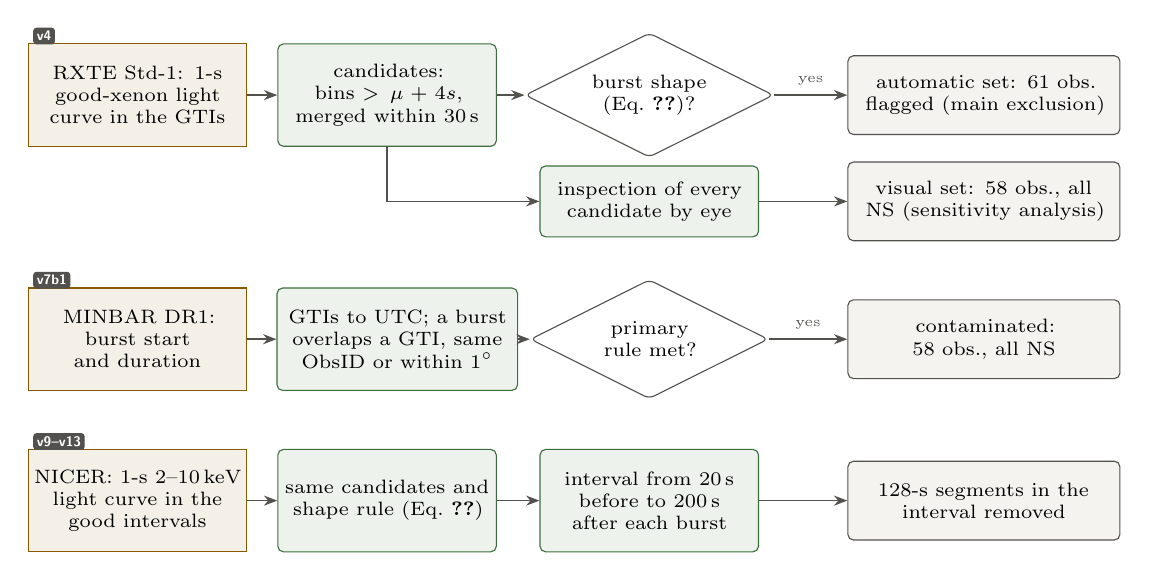
\begin{tikzpicture}[x=1cm, y=1cm,
  st/.style={fc proc, text width=2.62cm, minimum height=13mm},
  res/.style={fc, draw=inkgrey, fill=boxgrey, text width=3.3cm, minimum height=10mm},
  badge/.style={fc ver, anchor=south west}]
  % lane 1: Standard-1 detector (v4)
  \node[fc data, text width=2.62cm, minimum height=13mm] (a1) at (1.45,0) {RXTE Std-1: 1-s good-xenon light curve in the GTIs};
  \node[st] (a2) at (4.62,0)  {candidates: bins $>\mu+4s$, merged within 30\,s};
  \node[fc dec, text width=2.0cm, aspect=2.0] (a3) at (7.95,0) {burst shape (Eq.~\ref{eq:burst})?};
  \node[res] (a5) at (12.2,0) {automatic set: 61 obs.\ flagged (main exclusion)};
  \node[st, minimum height=9mm] (a4) at (7.95,-1.35) {inspection of every candidate by eye};
  \node[res] (a6) at (12.2,-1.35) {visual set: 58 obs., all NS (sensitivity analysis)};
  \draw[fc arr] (a1) -- (a2); \draw[fc arr] (a2) -- (a3);
  \draw[fc arr] (a3) -- node[font=\tiny, above] {yes} (a5);
  \draw[fc arr] (a2.south) |- (a4.west); \draw[fc arr] (a4) -- (a6);
  % lane 2: MINBAR (v7b1)
  \node[fc data, text width=2.62cm, minimum height=13mm] (b1) at (1.45,-3.1) {MINBAR DR1: burst start and duration};
  \node[st, text width=2.9cm] (b2) at (4.75,-3.1) {GTIs to UTC; a burst overlaps a GTI, same ObsID or within $1^\circ$};
  \node[fc dec, text width=2.0cm, aspect=2.0] (b3) at (7.95,-3.1) {primary rule met?};
  \node[res] (b5) at (12.2,-3.1) {contaminated: 58 obs., all NS};
  \draw[fc arr] (b1) -- (b2); \draw[fc arr] (b2) -- (b3);
  \draw[fc arr] (b3) -- node[font=\tiny, above] {yes} (b5);
  % lane 3: NICER (v9--v13)
  \node[fc data, text width=2.62cm, minimum height=13mm] (c1) at (1.45,-5.15) {NICER: 1-s 2--10\,keV light curve in the good intervals};
  \node[st] (c2) at (4.62,-5.15) {same candidates and shape rule (Eq.~\ref{eq:burst})};
  \node[st] (c3) at (7.95,-5.15) {interval from 20\,s before to 200\,s after each burst};
  \node[res] (c4) at (12.2,-5.15) {128-s segments in the interval removed};
  \draw[fc arr] (c1) -- (c2); \draw[fc arr] (c2) -- (c3); \draw[fc arr] (c3) -- (c4);
  % badges
  \foreach \n/\v in {a1/v4, b1/v7b1, c1/{v9--v13}} \node[badge] at ([xshift=2pt, yshift=-0.4pt]\n.north west) {\v};
\end{tikzpicture}

\caption{Burst screening: the Standard-1 detector (v4), the MINBAR match (v7b1) and the NICER rule (v9--v13), which removes
segments rather than observations. Counts refer to the 456 v2 observations.}\label{fig:burstflow}
\end{figure}

\paragraph{Standard-1 detector (v4, \file{17_v4_burst_detect.py}).} The 1\,s light curve $r(t)$ is the sum of good-xenon
counts of the spectrum's PCUs over complete 1\,s bins inside the GTIs. With $\mu$ and $s$ the mean and standard deviation of
all bins, bins with $r>\mu+4s$ are candidates, and candidates closer than 30\,s are merged. For an event with peak
$r_\mathrm{pk}$ and persistent level $r_0$ (median of the preceding 60\,s), $A=r_\mathrm{pk}-r_0$ and $L_q=r_0+qA$,
\begin{equation}
\text{burst}\iff r_\mathrm{pk}\ge1.5\,r_0\ \wedge\ t_\mathrm{rise}\le10\,\mathrm{s}\ \wedge\ 3\le t_{1/2}\le300\,\mathrm{s}\ \wedge\ n_{25}\ge3,\label{eq:burst}
\end{equation}
where $t_\mathrm{rise}$ is measured from the last time below $L_{0.25}$ to the peak, $t_{1/2}$ from the peak to the first time
below $L_{0.5}$, and $n_{25}$ counts the contiguous bins above $L_{0.25}$ (\code{V4_BURST} in \file{config.py}). The burst
interval runs from the last time before the peak below $L_{0.25}$ to the first time after it below $L_{0.1}$. Every
candidate was also inspected by eye (\file{results/v4/burst_visual.csv}).

\paragraph{MINBAR match (v7b1, \file{31_v7b1_minbar.py}).} The spectrum GTIs (mission time, TT) are converted to MJD(TT) and
then to UTC with \code{astropy} (\code{v7lib.gti_utc}). A MINBAR burst occupies $[T,T+\mathrm{dur}]$, with 300\,s when the
duration is missing. Under the primary rule, an observation is contaminated if a burst interval overlaps a GTI and the burst
either has the same ObsID or comes from within $1^\circ$ (the PCA field of view) of the source. The literal planned rule
(any burst from anywhere) is a sensitivity set. \file{32_v7b1_replace.py} builds a further sensitivity sample by replacing
each contaminated observation with the next MINBAR-clean candidate of the same time group.

\paragraph{How the flags are used.} In the RXTE analyses, flagged observations stay in the main sample and are removed only
in sensitivity analyses (\file{18_v4_burst_exclusion.py}, \file{33_v7b1_exclusion.py}). The state index (below) is
different: it drops every Standard-1 row that overlaps a burst interval, starting 20\,s before the burst. For NICER, the
segments near a detected burst are removed (\cref{sec:nicer}).

% -----------------------------------------------------------------------------------------------------
\subsection{Low-frequency timing from Standard-1 (v5--v10)}\label{sec:std1timing}
\Cref{fig:timingflow} shows the timing chain. It is shared, with different constants, by RXTE event mode and NICER.

\begin{figure}[htbp]
\centering
\begin{tikzpicture}[x=1cm, y=1cm,
  st/.style={fc proc, text width=2.62cm, minimum height=16mm},
  badge/.style={fc ver, anchor=south west}]
  \node[fc data, text width=2.62cm, minimum height=16mm] (fs) at (1.45,0) {Std-1 \file{FS46_*}: 128-s rows, 1024 bins of 0.125\,s per PCU};
  \node[st] (rw) at (4.62,0) {rows fully inside a spectrum GTI; PCU on if all eight 16-s blocks have counts};
  \node[st] (bk) at (7.79,0) {mean source counts per bin $s=\bar c-n_\mathrm{det}\,b\,\Delta t$ (Std-2 background)};
  \node[st] (ft) at (10.96,0) {DFT per PCU; powers divided by $\sinc^2(j/N)$};
  \node[st] (cs) at (14.13,0) {cospectrum: two groups (v5) or all PCU pairs (v6, Eq.~\ref{eq:allpairs})};
  \foreach \a/\b in {fs/rw,rw/bk,bk/ft,ft/cs} \draw[fc arr] (\a) -- (\b);
  \node[st] (fb) at (14.13,-2.45) {fractional variance $f_\mathcal{B}$ per row and band (Table~\ref{tab:timingbands})};
  \node[st] (md) at (10.96,-2.45) {median over valid rows ($\ge3$ rows, else missing)};
  \node[st] (tk) at (7.79,-2.45) {$T_k=\sgn(f)\sqrt{|f|}$, $k=1,2,3$; $T_\mathrm{tot}$};
  \node[st] (nu) at (4.62,-2.45) {$\nu_c$: $\nu P_\nu$ centroid over 9 log bins (Eq.~\ref{eq:nuc})};
  \node[fc, draw=inkgrey, fill=boxgrey, text width=2.62cm, minimum height=16mm] (out) at (1.45,-2.45) {\file{timing_features.csv} (v5), \file{timing_v6.csv} (v6)};
  \draw[fc arr] (cs) -- (fb); \foreach \a/\b in {fb/md,md/tk,tk/nu,nu/out} \draw[fc arr] (\a) -- (\b);
  \node[st, text width=4.2cm, minimum height=12mm] (sti) at (10.96,-4.6) {state index: 0.1--4\,Hz rms from pair rows only, burst rows removed (Eq.~\ref{eq:state})};
  \node[fc, draw=inkgrey, fill=boxgrey, text width=2.62cm, minimum height=12mm] (so) at (7.0,-4.6) {\file{results/v7a/states.csv}};
  \draw[fc arr] (fb.south) |- (sti.east); \draw[fc arr] (sti) -- (so);
  \foreach \n/\v in {fs/v5, rw/v5, bk/v5, ft/v5, cs/{v5, v6}, fb/v5, md/v5, tk/v5, nu/v6, sti/v7a}
     \node[badge] at ([xshift=2pt, yshift=-0.4pt]\n.north west) {\v};
\end{tikzpicture}
\caption{Standard-1 timing chain (\file{v5lib.py}, \file{v6lib.py}, \file{v7lib.py}; scripts \file{26}, \file{29},
\file{34}, \file{42}, \file{53}). No new download is needed: the Standard-1 files were already fetched for the dead time.}
\label{fig:timingflow}
\end{figure}

\paragraph{Rows, detectors and background.} A Standard-1 row holds $N=1024$ bins of $\Delta t=0.125$\,s (128\,s) per PCU.
Only rows lying completely inside a spectrum GTI are used, with a 1\,ms tolerance (\code{v5lib.std1_rows}). A PCU is
\emph{on} in a row if each of the eight 128-bin blocks has at least one count (\code{v5lib.pcus_on}). The background rate per
PCU is taken from the Standard-2 background spectrum, $b=\sum_cC^b_c/(t_bN_{\mathrm{PCU},b})$, and assumed equal for all
PCUs. For counts $c_n$ summed over $n_\mathrm{det}$ detectors, the mean source counts per bin is
$s=\bar c-n_\mathrm{det}\,b\,\Delta t$; a row with any $s\le0$ is invalid.

\paragraph{Fourier conventions.} $X_j=\sum_nc_ne^{-2\pi ijn/N}$ for $j=0,\dots,N/2$ (\code{numpy.fft.rfft}), with
$\nu_j=j/(N\Delta t)$, i.e.\ $j/128$\,Hz. By Parseval's relation, $\frac{2}{N^2}\sum_{j\in\mathcal B}|X_j|^2$ is the variance
contributed by band $\mathcal B$. Binning multiplies the Fourier amplitude by $\sinc(j/N)=\sin(\pi j/N)/(\pi j/N)$, so every
power is divided by $\sinc^2(j/N)$.

\paragraph{Cospectra instead of power spectra.} Counting noise in different detectors is uncorrelated, so the
\emph{cross} spectrum between detectors has zero expected value without source variability. The Poisson and dead-time
noise level therefore never has to be modelled.
\begin{itemize}
\item \textbf{v5 (two groups, \code{v5lib.row_features}).} The PCUs that are on are sorted; those in even positions form
group A and those in odd positions group B (at least 2 PCUs). With summed counts $x,y$, transforms $X,Y$ and source means
$s_x,s_y$: $f_\mathcal B=\frac{2}{N^2}\sum_{j\in\mathcal B}\Re(X_jY_j^*)/\sinc^2(j/N)\big/(s_xs_y)$.
\item \textbf{v6 (all pairs, \code{v6lib.allpairs_row}).} Every pair of the $n$ PCUs that are on is used, through the closed
form
\begin{equation}
f_\mathcal B=\frac{\frac{2}{N^2}\sum_{j\in\mathcal B}\frac{|\sum_pX_{p,j}|^2-\sum_p|X_{p,j}|^2}{2\sinc^2(j/N)}}{\frac{(\sum_ps_p)^2-\sum_ps_p^2}{2}}.\label{eq:allpairs}
\end{equation}
Rows with one PCU on use the auto-power with a Poisson level, $\bigl(|X_j|^2-N\bar c\bigr)/\sinc^2(j/N)$ divided by $s^2$,
but only below 500\,c\,s$^{-1}$; brighter single-PCU rows are invalid. In synthetic tests the noise variance falls by
31--41\% for 3--5 PCUs, without bias.
\end{itemize}

\paragraph{From rows to features.} For each observation, the median over valid rows is taken in each band; with fewer than 3
valid rows the features are missing. The features are signed square roots (fractional rms, slightly negative when the
signal is below the noise):
\begin{equation}
\begin{gathered}
T_k=\sgn\bigl(\median_rf_{k,r}\bigr)\sqrt{\bigl|\median_rf_{k,r}\bigr|}\quad(k=1,2,3),\\
T_\mathrm{tot}=\sgn(F)\sqrt{|F|},\qquad F=\textstyle\sum_k\median_rf_{k,r}.
\end{gathered}\label{eq:signedsqrt}
\end{equation}
The bands are listed in \cref{tab:timingbands}. As a check, the v5 cospectral $T_2$ agrees with the conventional auto-power
estimate at Spearman 0.970 (276 observations with 20--500 source c\,s$^{-1}$\,PCU$^{-1}$).

\paragraph{Characteristic frequency $\nu_c$ (v6, \code{v6lib.nu_centroid}).} Nine logarithmic Fourier-index bins
$[1,1],[2,3],[4,7],\dots,[256,511]$ are formed. $P_b$ is the median over rows of the fractional variance in bin $b$; the bin
centre is $\nu_b=\sqrt{j_\mathrm{lo}j_\mathrm{hi}}/128$\,Hz and its width in $\ln\nu$ is
$\Delta_b=\ln\bigl((j_\mathrm{hi}+0.5)/(j_\mathrm{lo}-0.5)\bigr)$. Then
\begin{equation}
\ln\nu_c=\frac{\sum_bw_b\ln\nu_b}{\sum_bw_b},\qquad w_b=\frac{\max(P_b,0)}{\Delta_b},\label{eq:nuc}
\end{equation}
missing if $T^\ast_\mathrm{tot}<0.05$ or $\sum_bw_b\le0$. $\nu_c$ is the frequency around which most variability power per
logarithmic frequency interval lies: a model-free stand-in for a break frequency. (NICER uses 13 octave bins and does not
divide by $\Delta_b$; \cref{sec:nicer}.)

\paragraph{State index (v7a, \code{v7lib.state_rms}).} The 0.1--4\,Hz fractional rms ($j=13$--511) is computed with
\cref{eq:allpairs} from rows with at least two PCUs only, after removing every row that overlaps a burst interval
$[t_\mathrm{start}-20\,\mathrm{s},\ t_\mathrm{end}]$ (MINBAR field-of-view rule and the v4 detector). With
$\rho=\sgn(\median_rf)\sqrt{|\median_rf|}$,
\begin{equation}
\text{state}=\begin{cases}\text{hard-like}&\rho>0.10\\\text{soft-like}&\rho<0.075\\\text{intermediate}&\text{otherwise}\end{cases}
\qquad(\text{unknown with fewer than 3 rows}).\label{eq:state}
\end{equation}
The thresholds are those of \citet[Table~2]{RemillardMcClintock2006}, which are defined for 0.1--10\,Hz. The 4\,Hz Nyquist
limit of Standard-1 makes $\rho$ slightly low, so ``hard-like'' is conservative. A sanity gate must pass before the states are
used: at least two thirds of the XTE J1118+480 observations must be hard-like, and two thirds of the Z-source observations
(Cyg X-2, GX 17+2) soft-like.

\begin{table}[htbp]
\centering\small
\caption{Timing bands (Fourier index $j$; $\nu_j=j/128$\,Hz for Standard-1 and NICER, $j/16$\,Hz for event mode).}\label{tab:timingbands}
\begin{tabular}{@{}l l l l l@{}}
\toprule
Band & $j$ & Frequency [Hz] & Data & Setting \\
\midrule
$T_1$ & 2--12 & 0.016--0.094 & Std-1, NICER & \code{V5_BANDS_J}, \code{V9_T_BANDS_J} \\
$T_2$ & 13--128 & 0.10--1.0 & Std-1, NICER & \\
$T_3$ & 129--511 & 1.0--4.0 & Std-1, NICER & \\
state (v7a) & 13--511 & 0.10--4.0 & Std-1 & \code{V7_RMS_J} \\
state (v9+) & 13--1280 & 0.10--10 & NICER & \code{V9_STATE_J} \\
white-noise monitor & 12288--16383 & 96--128 & NICER & \code{V9_WHITE_J} \\
LC & 16--63 & 1--4 & event mode & \code{V8_HF_BANDS_J} \\
HF1 & 64--1023 & 4--64 & event mode & \\
HF2 & 1024--8191 & 64--512 & event mode & \\
HF3 & 8192--16383 & 512--1024 & event mode & \\
NULL & 24576--32767 & 1536--2048 & event mode & \\
\bottomrule
\end{tabular}
\end{table}

% -----------------------------------------------------------------------------------------------------
\subsection{High-frequency timing from event mode (v8c)}\label{sec:eventmode}
\file{43_v8c_events.py} first surveys the \file{SE*.evt.gz} files in each \file{pca/} directory, reading only their headers
with an HTTP range request. A file qualifies if \code{DATAMODE} matches \verb|^E_\d+us_\d+M_0_\d+s$|, \code{TDDES2} contains
all six anode chains, \code{TIMEDEL}~$\le2^{-12}$\,s and a \code{PCUID} column exists (\code{v8lib.mode_qualifies}). If
several modes qualify, the one with the largest total size is downloaded (2.4\,GB in total). Events are binned at
$2^{-12}$\,s (Nyquist 2048\,Hz) into 16\,s segments ($N=65536$) that lie inside both the spectrum GTIs and the event-file GTIs
and do not overlap a burst. A PCU is on if each 1\,s sub-interval has an event, and $\ge2$ PCUs are required.

Per segment $r$, the band numerator is $\mathrm{num}_{\mathcal B,r}=\frac{2}{N^2}\sum_{j\in\mathcal B}$(all-pairs cross
power) and the denominator $\mathrm{den}_r=\sum_{p<q}s_ps_q$. Single 16\,s segments of faint sources gave unstable ratios,
so the observation value is the ratio of means (\code{v8lib.hf_summary}):
\begin{equation}
\hat R_\mathcal B=\frac{\sum_r\mathrm{num}_{\mathcal B,r}}{\sum_r\mathrm{den}_r},\qquad
\widehat{\mathrm{SE}}=\frac{1}{\sum_r\mathrm{den}_r}\sqrt{\frac{n}{n-1}\sum_r\bigl(\mathrm{num}_{\mathcal B,r}-\hat R_\mathcal B\,\mathrm{den}_r\bigr)^2}.\label{eq:ratioofmeans}
\end{equation}
This replaced the planned mean of per-segment ratios after an implementation check, before any model. The features are
$\sgn(\hat R)\sqrt{|\hat R|}$ for LC, HF1, HF2 and HF3. Quality requires at least 10 segments and
$|\hat R_\mathrm{NULL}/\widehat{\mathrm{SE}}|\le5$ in the empty 1536--2048\,Hz band. After results were seen, a correlated
white component was found; a post hoc correction subtracts the null-band power scaled by bandwidth. Output:
\file{data/v8c/processed/hf_features.csv}.

% -----------------------------------------------------------------------------------------------------
\subsection{Outputs of the RXTE chain}\label{sec:rxteoutputs}
\begin{itemize}
\item \file{data/<v>/processed/features.npz}: rebinned spectra and errors of the accepted observations (\cref{sec:datamodel}).
\item \file{data/<v>/observations.csv}: every tried candidate, with status, reason, header values, dead-time terms and
summary rates.
\item \file{data/<v>/processed/feature_definitions.csv}: grid edges and the definitions of A and B.
\item Timing: \file{data/v5/processed/timing_features.csv}, \file{data/v6/processed/timing_v6.csv},
\file{data/v8b/processed/external_states_timing.csv}, \file{data/v10/processed/rxte_timing_table.csv}.
\item Bursts and states: \file{results/v4/burst_flags.csv}, \file{results/v7b1/minbar_flags.csv},
\file{results/v7a/states.csv}.
\end{itemize}

% =====================================================================================================
\section{NICER and MAXI processing}\label{sec:nicermaxi}
% =====================================================================================================

% -----------------------------------------------------------------------------------------------------
\subsection{NICER/XTI: from event files to features (v9--v13)}\label{sec:nicer}
The NICER chain (\cref{fig:nicerflow}) works on cleaned event files without HEASoft. It uses the same cospectral idea
as Standard-1, with the seven NICER measurement/power units (MPUs) as detectors. HEASoft enters only for the 3C50
background (\cref{sec:3c50}). Library code: \file{v9lib.py} (parser, segments, features), \file{v10lib.py} (tail and
background proxy), \file{v11lib.py} (streaming, Lorentzians).

\begin{figure}[htbp]
\centering
% NICER/XTI pipeline (v9--v13) and the version that added each step. Copied from report_en/figures/flowcharts (styles in workflow_report.tex).
% Row 1 left to right, row 2 right to left.
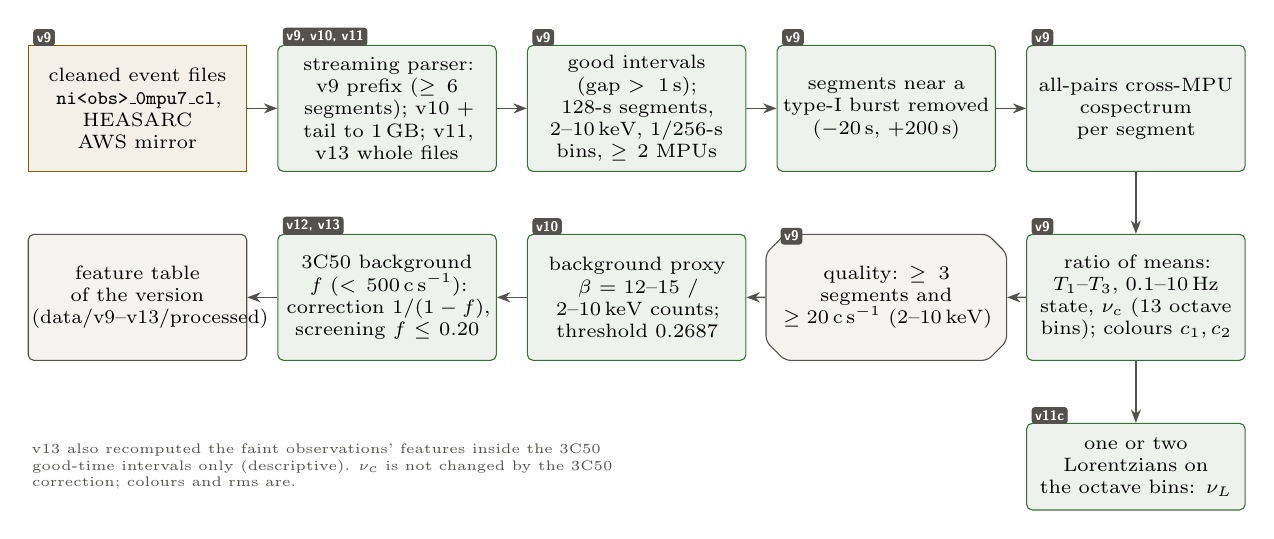
\begin{tikzpicture}[x=1cm, y=1cm,
  st/.style={fc proc, text width=2.62cm, minimum height=16mm},
  badge/.style={fc ver, anchor=south west}]
  % row 1: events to per-segment cospectra
  \node[fc data, text width=2.62cm, minimum height=16mm] (ev) at (1.45,0) {cleaned event files \texttt{ni<obs>\_0mpu7\_cl}, HEASARC AWS mirror};
  \node[st] (rd)  at (4.62,0)  {streaming parser: v9 prefix ($\ge6$ segments); v10 + tail to 1\,GB; v11, v13 whole files};
  \node[st] (seg) at (7.79,0)  {good intervals (gap $>1$\,s); 128-s segments, 2--10\,keV, 1/256-s bins, $\ge2$ MPUs};
  \node[st] (bst) at (10.96,0) {segments near a type-I burst removed ($-20$\,s, $+200$\,s)};
  \node[st] (cos) at (14.13,0) {all-pairs cross-MPU cospectrum per segment};
  \foreach \a/\b in {ev/rd,rd/seg,seg/bst,bst/cos} \draw[fc arr] (\a) -- (\b);
  % row 2: observation features, quality, background
  \node[st, text width=2.62cm] (of) at (14.13,-2.4) {ratio of means: $T_1$--$T_3$, 0.1--10\,Hz state, $\nu_c$ (13 octave bins); colours $c_1,c_2$};
  \node[fc gate, text width=2.62cm, minimum height=16mm] (qg) at (10.96,-2.4) {quality: $\ge3$ segments and $\ge20$\,c\,s$^{-1}$ (2--10\,keV)};
  \node[st] (bp)  at (7.79,-2.4) {background proxy $\beta$ = 12--15 / 2--10\,keV counts; threshold 0.2687};
  \node[st] (c50) at (4.62,-2.4) {3C50 background $f$ ($<500$\,c\,s$^{-1}$): correction $1/(1-f)$, screening $f\le0.20$};
  \node[fc, draw=inkgrey, fill=boxgrey, text width=2.62cm, minimum height=16mm] (tab) at (1.45,-2.4) {feature table of the version (\file{data/v9}--\file{v13/processed})};
  \draw[fc arr] (cos) -- (of);
  \foreach \a/\b in {of/qg,qg/bp,bp/c50,c50/tab} \draw[fc arr] (\a) -- (\b);
  % side branch: Lorentzian fits
  \node[st, minimum height=11mm] (lz) at (14.13,-4.55) {one or two Lorentzians on the octave bins: $\nu_L$};
  \draw[fc arr] (of) -- (lz);
  \node[fc note, text width=7.6cm, anchor=west] at (1.45-1.38,-4.55)
     {v13 also recomputed the faint observations' features inside the 3C50 good-time intervals only (descriptive).
      $\nu_c$ is not changed by the 3C50 correction; colours and rms are.};
  % version badges
  \foreach \n/\v in {ev/v9, rd/{v9, v10, v11}, seg/v9, bst/v9, cos/v9, of/v9, qg/v9, bp/v10, c50/{v12, v13}, lz/v11c}
     \node[badge] at ([xshift=2pt, yshift=-0.4pt]\n.north west) {\v};
\end{tikzpicture}

\caption{NICER/XTI feature pipeline: top row left to right, then bottom row right to left. The v9 steps were frozen before
the observations of v11 were read, and the whole chain, including 3C50, before those of v13.}\label{fig:nicerflow}
\end{figure}

\paragraph{Step 1: read the events.} \code{v9lib.PrefixParser} turns the compressed byte stream into event arrays
(\cref{sec:get-nicer}):
\begin{enumerate}
\item \code{zlib} (gzip mode) decompresses each new piece into a buffer;
\item once the buffer holds them, the primary and \code{EVENTS} headers are parsed from 2880-byte blocks;
\item \code{row_dtype} builds a big-endian numpy record type from \code{TFIELDS}, \code{TTYPEn} and \code{TFORMn}, checking
that the row length equals \code{NAXIS1};
\item complete rows are converted and only \code{TIME}, \code{PI} and \code{DET_ID} are kept;
\item the parse is \emph{complete} when \code{NAXIS2} rows have been read.
\end{enumerate}
Events are expected in time order; if they are not, they are sorted (and flagged).

\paragraph{Step 2: good intervals and segments.} A good interval is a maximal stretch with no gap longer than 1\,s between
consecutive events of any energy (\code{v9lib.good_intervals}). Each interval $[a,b]$ is cut into consecutive 128\,s
segments starting at $a$. Only 2--10\,keV events (PI 200--999; PI is in units of 10\,eV) are used for timing. The detector
of an event is its MPU, $m=\lfloor\mathtt{DET\_ID}/10\rfloor\in\{0,\dots,6\}$. Events are binned at $1/256$\,s ($N=32768$,
Nyquist 128\,Hz). An MPU is on in a segment if each of the eight 16\,s blocks contains a 2--10\,keV event. A segment needs at
least 2 MPUs on.

\paragraph{Step 3: bursts.} The 1\,s 2--10\,keV light curve inside the good intervals (\code{v9lib.lc_1s}) is searched with
the RXTE burst rule (\cref{eq:burst}, \code{v9lib.burst_events}). Every segment that overlaps
$[t_\mathrm{start}-20\,\mathrm{s},\ t_\mathrm{end}+200\,\mathrm{s}]$ of a detected burst is skipped; the number skipped is
stored as \code{n_seg_burst_removed}.

\paragraph{Step 4: per-segment statistics (\code{v9lib.segment_stats}).} For the $n$ MPUs that are on, with mean counts per
bin $s_m$ (no background subtraction) and transforms $X_{m,j}$, the all-pairs cross power is
$\mathrm{cross}_j=\bigl(|\sum_mX_{m,j}|^2-\sum_m|X_{m,j}|^2\bigr)/(2\sinc^2(j/N))$ (\cref{eq:allpairs}). Each segment
stores a numerator $\mathrm{num}_{\mathcal B,r}=\frac{2}{N^2}\sum_{j\in\mathcal B}\mathrm{cross}_j$ for every band and for each
of the 13 octave bins, and the denominator $\mathrm{den}_r=\sum_{m<m'}s_ms_{m'}$.

\paragraph{Step 5: observation features (\code{v9lib.obs_features}).}
\begin{itemize}
\item \textbf{Timing.} Each band is combined over segments by the ratio of means with its delta-method error
(\cref{eq:ratioofmeans}), and converted to a signed square root. The bands are $T_1$, $T_2$, $T_3$, the state band
0.1--10\,Hz and the 96--128\,Hz white-noise monitor (\cref{tab:timingbands}).
\item \textbf{Colours.} \emph{All} events of all detectors inside the accepted segment windows are counted in PI 200--399
($A$, 2--4\,keV), 400--599 ($B$, 4--6\,keV) and 600--999 ($C$, 6--10\,keV); $c_1=B/A$ and $c_2=C/B$. The colours therefore
come from exactly the time windows used for timing.
\item \textbf{Count rate.} \code{rate_2_10} is the mean over segments of the 2--10\,keV counts of the MPUs that are on,
divided by 128\,s.
\item \textbf{$\nu_c$.} The 13 octave bins $k=0,\dots,12$ cover $j\in[2^k,2^{k+1}-1]$ (1/128--64\,Hz). With
$\ell_k=\sum_r\mathrm{num}_{k,r}/\sum_r\mathrm{den}_r$, $w_k=\max(\ell_k,0)$ and $\nu_k=2^{k+0.5}/128$\,Hz,
$\nu_c=\exp\bigl(\sum_kw_k\ln\nu_k/\sum_kw_k\bigr)$. It is missing if $\sqrt{\max(\sum_k\ell_k,0)}<0.05$. Unlike the RXTE
version (\cref{eq:nuc}), the weights are not divided by the bin width; for octave bins this matters only for the lowest bin.
\item \textbf{State.} \Cref{eq:state} is applied to the 0.1--10\,Hz rms, the full band of \citet{RemillardMcClintock2006}.
\item \textbf{Status.} \code{ok} needs at least 3 valid segments and \code{rate_2_10}~$\ge20$\,c\,s$^{-1}$; otherwise
\code{missing} or \code{excluded} (\cref{tab:qualityrules}).
\end{itemize}

\paragraph{Background proxy (v10, \code{v10lib.bkg_ratio}).} $\beta=N(\mathrm{PI}\,1200\text{--}1499)/N(\mathrm{PI}\,200\text{--}999)$
over the whole file, the ratio of 12--15\,keV to 2--10\,keV events. Above 12\,keV the source contributes little, so a high
$\beta$ indicates background. The threshold, frozen at 0.2687, is the 99th percentile of $\beta$ among observations brighter
than 500\,c\,s$^{-1}$, where the background is negligible. It was used only for sensitivity analyses in v10 and v11.

\paragraph{Per-bin errors and Lorentzian fits (v11c, \code{v11lib}).}\label{sec:lorentz} \code{lb_se} gives a delta-method
error for each octave-bin variance $\ell_k$. \code{fit_lorentz} fits one or two zero-centred Lorentzians whose integrated
variance in bin $[\nu^\mathrm{lo}_k,\nu^\mathrm{hi}_k]$ (edges $(j\mp0.5)/128$\,Hz) is
\begin{equation}
L_k(r^2,\Delta)=r^2\,\frac{2}{\pi}\Bigl[\arctan\frac{\nu^\mathrm{hi}_k}{\Delta}-\arctan\frac{\nu^\mathrm{lo}_k}{\Delta}\Bigr],\qquad\Delta\in[1/128,\,128]\ \mathrm{Hz}.\label{eq:lorentz}
\end{equation}
The fit is weighted least squares in log-parameters (\code{scipy.optimize.least_squares}), with four starting points per
model; at least 6 usable bins are required. With $\mathrm{BIC}=\chi^2+k\ln n$, two components are chosen if
$\mathrm{BIC}_1-\mathrm{BIC}_2>6$. The width of the lowest-frequency component is $\nu_L$.

\paragraph{Reading modes and storage.} v9 parsed only a prefix of each file, stopping at 6 segments (\cref{tab:nicermodes}).
v10 appended the tail up to 1\,GB and re-parsed prefix and tail as one stream (\code{v10lib.read_full}); 366 of the 368 N1
observations remained \code{ok}. v11 and v13 streamed whole files into the frozen \code{obs_features} without storing them
(\code{v11lib.obs_features_stream}), with 64\,MB requests in windows of 6 concurrent requests consumed in order. The fetch
scripts keep a checkpoint (\file{observations_partial.jsonl}), so an interrupted run resumes without re-reading finished
observations.

% -----------------------------------------------------------------------------------------------------
\subsection{NICER background: 3C50 correction and screening (v12, v13)}\label{sec:3c50}
\Cref{fig:3c50flow} shows the background step. It is applied only to observations fainter than 500\,c\,s$^{-1}$ in
2--10\,keV; for brighter ones the background is treated as negligible ($f=0$).

\begin{figure}[htbp]
\centering
\begin{tikzpicture}[x=1cm, y=1cm,
  st/.style={fc proc, text width=2.62cm, minimum height=16mm},
  badge/.style={fc ver, anchor=south west}]
  \node[fc data, text width=2.62cm, minimum height=16mm] (in) at (1.45,0) {accepted NICER obs.\ (\code{ok}) with rate $<500$\,c\,s$^{-1}$};
  \node[st] (dl) at (4.62,0) {WSL: \code{curl} \code{_cl} and \code{_ufa} files (3 tries); SHA256 to the log};
  \node[st] (bg) at (7.79,0) {\code{nibackgen3C50}, CALDB library, \code{gainepoch=AUTO}};
  \node[st] (sp) at (10.96,0) {keep \file{tot_<o>.pi}, \file{bkg_<o>.pi}; delete event files};
  \node[st] (fr) at (14.13,0) {band fractions $f_\mathcal{X}=\sum B/\sum T$ for $\mathcal X$ = A, B, C, T};
  \foreach \a/\b in {in/dl,dl/bg,bg/sp,sp/fr} \draw[fc arr] (\a) -- (\b);
  \node[fc dec, text width=1.9cm, aspect=1.9] (q) at (14.13,-2.55) {3C50 ok and $f_\mathrm{T}\le0.20$?};
  \node[st] (co) at (10.2,-2.55) {correct rms by $1/(1-f_\mathrm{T})$, colours band by band (Eq.~\ref{eq:3c50}); new state};
  \node[fc no, text width=2.62cm, minimum height=10mm] (ex) at (14.13,-4.5) {excluded: 3C50 failed or $f_\mathrm{T}>0.20$};
  \node[fc, draw=inkgrey, fill=boxgrey, text width=3.1cm, minimum height=16mm] (out) at (6.3,-2.55) {\file{nicer_corrected_screened.csv} (v12); v13 test table};
  \node[fc data, text width=2.62cm, minimum height=12mm] (br) at (1.45,-2.55) {bright obs.: $f=0$, kept unchanged};
  \draw[fc arr] (fr) -- (q); \draw[fc arr] (q) -- node[fc note, above] {yes} (co); \draw[fc arr] (q) -- node[fc note, right] {no} (ex);
  \draw[fc arr] (co) -- (out); \draw[fc arr] (br) -- (out);
  \foreach \n/\v in {in/v12, dl/v12, bg/v12, sp/v12, fr/v12, co/{v12, frozen in v13}}
     \node[badge] at ([xshift=2pt, yshift=-0.4pt]\n.north west) {\v};
\end{tikzpicture}
\caption{3C50 background step (\file{58_v12_bkg.py}, \file{62_v13_bkg.py}, \file{v12_bkg3c50.sh}; correction in
\code{corrected} of \file{59_v12_analysis.py}, copied unchanged into \file{63_v13_analysis.py}).}\label{fig:3c50flow}
\end{figure}

\paragraph{Running 3C50.} The 3C50 model \citep{Remillard2022} estimates the background spectrum of an observation from a
library of blank-sky observations, selected by background-sensitive count rates measured in the observation itself (hence
the unfiltered \code{_ufa} file). For each faint observation the Python driver calls, through \code{wsl -d Ubuntu-22.04}, the shell
script \file{v12_bkg3c50.sh} with the ObsID, the cleaned and unfiltered URLs, an output folder and the CALDB folder. The
script activates the HEASoft conda environment and points \code{CALDB}, \code{CALDBCONFIG} and \code{CALDBALIAS} at the
unpacked library. It downloads the two files into \file{/tmp/bkg3c50/<obsid>/xti/event_cl/} and unzips them. It then runs
\begin{verbatim}
nibackgen3C50 rootdir=/tmp/bkg3c50 obsid=<obsid>
              bkgidxdir=CALDB bkglibdir=CALDB gainepoch=AUTO clobber=yes chatter=1
              totspec=tot_<obsid> bkgspec=bkg_<obsid>
\end{verbatim}
copies the two spectra out and deletes the working folder. The driver reads the spectra (\code{RATE}, or \code{COUNTS}
divided by \code{EXPOSURE}) and sums them in the PI bands A, B, C and T (200--999). It records the band rates $T_\mathcal X$
and $B_\mathcal X$, the fractions $f_\mathcal X=B_\mathcal X/T_\mathcal X$ and the 3C50 exposure in
\file{data/v12/processed/bkg3c50.csv}. Six workers run in parallel, and a checkpoint file makes the step resumable.

\paragraph{Failures.} In v12, 362 of the 503 faint observations gave spectra; 141 failed, mostly because the tool rejects
data processed with the oldest gain calibration. In v13, 109 of 148 succeeded. Failed observations are excluded from the
corrected analyses.

\paragraph{Correction and screening.} An observation is kept if it is bright, or if 3C50 succeeded with
$f_\mathrm{T}\le0.20$; thresholds 0.10 and 0.30 are sensitivity variants. For kept faint observations,
\begin{equation}
T_k'=\frac{T_k}{1-f_\mathrm{T}}\quad(k=1,2,3,\text{state}),\qquad c_1'=\frac{B(1-f_B)}{A(1-f_A)},\qquad c_2'=\frac{C(1-f_C)}{B(1-f_B)},\label{eq:3c50}
\end{equation}
and the state is re-classified with the corrected state rms. A fractional rms is normalised to the total mean count rate;
renormalising it to the source mean $S=(1-f)(S+B)$ multiplies it by $1/(1-f)$, assuming a constant background. $\nu_c$ is
not changed, because it depends only on the shape of the power spectrum. A check requires the 3C50 total 2--10\,keV rate to
be within 0.7--1.3 of the pipeline rate for at least 90\% of observations.

\paragraph{GTI-restricted variant (v13, descriptive).} For the faint v13 observations, the cleaned event files were kept
(\code{V13_KEEP_CL}). Their features were recomputed using only events inside the GTIs of the 3C50 total spectrum
(\code{gti_restricted} in \file{63_v13_analysis.py}), to check that the two time selections give the same picture.

% -----------------------------------------------------------------------------------------------------
\subsection{MAXI/GSC: daily light curves (v7c, v8d, v9c)}\label{sec:maxi}
MAXI points are days, not pointed observations. \Cref{fig:maxiflow} shows the chain.

\begin{figure}[htbp]
\centering
% MAXI/GSC pipeline (v7c, v8d, v9c) and the version that added each step. Copied from report_en/figures/flowcharts (styles in workflow_report.tex).
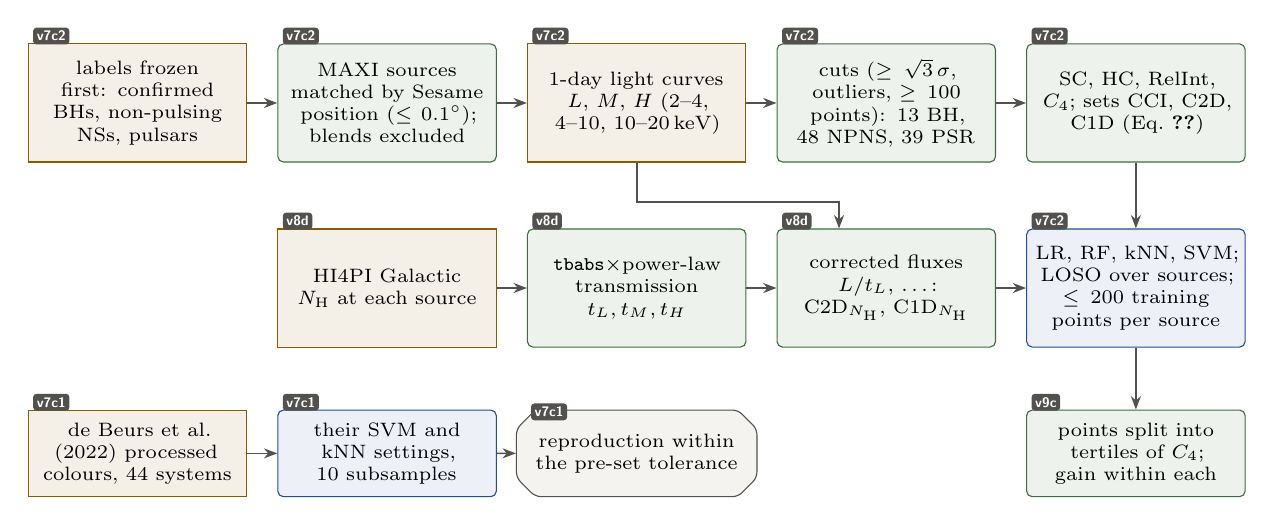
\begin{tikzpicture}[x=1cm, y=1cm,
  st/.style={fc proc, text width=2.62cm, minimum height=15mm},
  badge/.style={fc ver, anchor=south west}]
  % row 1: strict pipeline (v7c2)
  \node[fc data, text width=2.62cm, minimum height=15mm] (lab) at (1.45,0) {labels frozen first: confirmed BHs, non-pulsing NSs, pulsars};
  \node[st] (mt)  at (4.62,0)  {MAXI sources matched by Sesame position ($\le0.1^\circ$); blends excluded};
  \node[fc data, text width=2.62cm, minimum height=15mm] (lc) at (7.79,0) {1-day light curves $L$, $M$, $H$ (2--4, 4--10, 10--20\,keV)};
  \node[st] (cut) at (10.96,0) {cuts ($\ge\sqrt3\,\sigma$, outliers, $\ge100$ points): 13 BH, 48 NPNS, 39 PSR};
  \node[st] (ft)  at (14.13,0) {SC, HC, RelInt, $C_4$; sets CCI, C2D, C1D (Eq.~\ref{eq:maxi})};
  \foreach \a/\b in {lab/mt,mt/lc,lc/cut,cut/ft} \draw[fc arr] (\a) -- (\b);
  % row 2: absorption correction (v8d) feeding the same models
  \node[fc data, text width=2.62cm, minimum height=15mm] (nh) at (4.62,-2.35) {HI4PI Galactic $N_\mathrm{H}$ at each source};
  \node[st] (tr)  at (7.79,-2.35) {\texttt{tbabs}$\times$power-law transmission $t_L,t_M,t_H$};
  \node[st] (ftc) at (10.96,-2.35) {corrected fluxes $L/t_L$, \dots: C2D$_{N_\mathrm{H}}$, C1D$_{N_\mathrm{H}}$};
  \node[fc model, text width=2.62cm, minimum height=15mm] (md) at (14.13,-2.35) {LR, RF, kNN, SVM; LOSO over sources; $\le200$ training points per source};
  \draw[fc arr] (nh) -- (tr); \draw[fc arr] (tr) -- (ftc); \draw[fc arr] (ftc) -- (md);
  \draw[fc arr] (ft) -- (md);
  \draw[fc arr] (lc.south) -- ++(0,-0.5) -| ([xshift=-6mm]ftc.north);
  % row 3: strata (v9c) and the reproduction (v7c1)
  \node[st, text width=2.62cm, minimum height=11mm] (ter) at (14.13,-4.45) {points split into tertiles of $C_4$; gain within each};
  \draw[fc arr] (md) -- (ter);
  \node[fc data, text width=2.62cm, minimum height=11mm] (db) at (1.45,-4.45) {de Beurs et al.\ (2022) processed colours, 44 systems};
  \node[fc model, text width=2.62cm, minimum height=11mm] (dbm) at (4.62,-4.45) {their SVM and kNN settings, 10 subsamples};
  \node[fc gate, text width=2.62cm, minimum height=11mm] (dbr) at (7.79,-4.45) {reproduction within the pre-set tolerance};
  \draw[fc arr] (db) -- (dbm); \draw[fc arr] (dbm) -- (dbr);
  % badges
  \foreach \n/\v in {lab/v7c2, mt/v7c2, lc/v7c2, cut/v7c2, ft/v7c2, md/v7c2, nh/v8d, tr/v8d, ftc/v8d, ter/v9c, db/v7c1, dbm/v7c1, dbr/v7c1}
     \node[badge] at ([xshift=2pt, yshift=-0.4pt]\n.north west) {\v};
\end{tikzpicture}

\caption{MAXI/GSC pipeline: the strict pipeline (v7c2), the absorption correction (v8d), the colour strata (v9c) and the
reproduction of \citet{deBeurs2022} (v7c1), which uses their processed colours instead of this pipeline.}\label{fig:maxiflow}
\end{figure}

\paragraph{Source matching (\file{38_v7c2_select.py}).}
\begin{enumerate}
\item The label lists are frozen first: 25 BHs \citep{Marcel2026}, the 115 MINBAR bursters and the pulsar lists. Sources
with a pulse period in the Liu et al.\ HMXB or LMXB catalogues (CDS J/A+A/455/1165 and J/A+A/469/807) or in Patruno \&
Watts form the separate pulsar class. MINBAR bursters without a pulse period are the ``non-pulsing'' NSs (NPNS).
\item The MAXI source index is scraped from the 13 category pages \file{http://maxi.riken.jp/top/lc_<cat>.html}. Each entry
gives a name and a J-identifier, whose digits encode an approximate position (RA hhmm, Dec $\pm$dd.d).
\item Entries whose name contains ``with'' are blends of two sources and are removed. The remaining MAXI names are resolved
with Sesame. A label source matches a MAXI source within $0.1^\circ$ of the Sesame position, or within $0.3^\circ$ of the
J-name position if Sesame fails.
\item A MAXI source matched by label sources of different classes, or by several label sources that are not aliases of one
object, is excluded as ambiguous (\file{data/v7c/c2_sources_ambiguous.csv}).
\end{enumerate}

\paragraph{Light curves and cuts.} For every matched source the 1-day light curve
\file{<J>_g_lc_1day_all.dat} is downloaded (columns MJD, total flux and error, then $L$, $M$, $H$ with errors for 2--4,
4--10 and 10--20\,keV). The cuts of \citet{deBeurs2022} are then applied:
\begin{itemize}
\item every band must have flux/error $\ge\sqrt3$ and a positive error;
\item points with $L+M+H\ge$ mean $+\,10$\,sd of the source are dropped;
\item the source needs at least 100 remaining points.
\end{itemize}
Result: \file{data/v7c/maxi_points.csv} with 132\,057 points of 13 BH, 48 NPNS and 39 pulsar sources.

\paragraph{Features (\file{39_v7c2_analysis.py}).} Per point,
\begin{equation}
\mathrm{SC}=\frac{M-L}{M+L},\qquad\mathrm{HC}=\frac{H-L}{H+L},\qquad C_4=\frac{H-M}{H+M},\qquad
\mathrm{RelInt}=\frac{L+M+H}{Q_{99.99}(L+M+H)},\label{eq:maxi}
\end{equation}
where $Q_{99.99}$ is the 99.99th percentile over that source's points. The feature sets are CCI = (SC, HC, RelInt),
C2D = (SC, HC) and C1D = ($C_4$), the only colour without the 2--4\,keV band.

\paragraph{Absorption correction (v8d, \file{45_v8d_nh.py}, \file{v8d_heasoft.sh}).}
\begin{enumerate}
\item HEASoft \code{nh} gives the HI4PI column at each source position (\code{disio=0.1}; the weighted average
\code{avwnh} is used).
\item XSPEC computes photon fluxes of \code{tbabs*powerlaw} ($\Gamma=2$; \code{abund wilm}, \code{xsect vern}; a dummy
response from 0.5 to 30\,keV) in the three MAXI bands. The grid is $N_\mathrm{H}=0$ plus 200 logarithmic steps from
$10^{19}$ to $10^{23.5}$\,cm$^{-2}$.
\item The transmission is $t_\mathcal X(N_\mathrm H)=\Phi_\mathcal X(N_\mathrm H)/\Phi_\mathcal X(0)$, interpolated linearly
in $\log N_\mathrm H$.
\item The corrected fluxes $L/t_L$, $M/t_M$, $H/t_H$ give SC$'$, HC$'$, $C_4'$ and RelInt$'$ through \cref{eq:maxi} (sets
C2D$_{N_\mathrm H}$, C1D$_{N_\mathrm H}$, CCI$_{N_\mathrm H}$).
\end{enumerate}

\paragraph{Colour strata (v9c, \file{50_v9c_maxi_strata.py}).} The points are split into tertiles of $C_4$, and the
models are compared within each tertile.

\paragraph{Reproduction of de Beurs et al.\ (v7c1, \file{37_v7c1_repro.py}).} Their processed colours of 44 systems and
their ten 20\% subsamples are used with their three-class settings (BH, NPNS, pulsar): kNN with $k=24$ and SVM with $C=0.655$,
$\gamma=0.585$. The reproduction counts as successful if, for each algorithm, the number of correctly classified systems
is within 2 of the published number (kNN 37, SVM 36) and the number of correct BHs within 1 (6 and 5)
(\code{V7_REPRO_TOL_SOURCES}, \code{V7_REPRO_TOL_BH}). Otherwise the script stops.

% =====================================================================================================
\section{Data model: from stored tables to design matrices}\label{sec:datamodel}
% =====================================================================================================

Every model in the project sees the same three objects: a design matrix, a label vector and a source vector. This section
defines them, shows how they are assembled from the stored files, and lists the controls that keep information about a
test source out of its own prediction.

\subsection{Notation}\label{sec:notation}
An analysis uses $n$ observations of $S$ sources.
\begin{itemize}
\item $\Xm\in\mathbb R^{n\times p}$, the \textbf{design matrix}. Row $i$ is one observation: an RXTE ObsID, a NICER ObsID or
one MAXI day. Column $\ell$ is one feature.
\item $\yv\in\{0,1\}^n$, the labels, $y_i=1$ for a BH. Every observation inherits the label of its source.
\item $\gv\in\{1,\dots,S\}^n$, the source (group) of each row; $n_k$ is the number of rows of source $k$, and $S_1$ and $S_0$
are the numbers of BH and NS sources.
\item $\wv$, the sample weights used in a fit (\cref{sec:weights}).
\item $\hat s_i\in[0,1]$, the \textbf{out-of-fold (OOF) score} (``BH score''), always produced by a model fitted without any
observation of source $g_i$. Scores are model outputs, not calibrated probabilities.
\item \textbf{Source score and decisions:}
\begin{equation}
\bar s_k=\frac1{n_k}\sum_{i:g_i=k}\hat s_i,\qquad\hat Y_k=\indic{\bar s_k\ge t},\qquad\hat y_i=\indic{\hat s_i\ge t},\qquad t=0.5.\label{eq:sourcescore}
\end{equation}
The only exception is the nested procedure of v4a, which selects a threshold inside the training sources
(\cref{sec:nested}). Observations of one source are never multiplied together as independent evidence.
\end{itemize}

% -----------------------------------------------------------------------------------------------------
\subsection{Assembling a design matrix}\label{sec:buildX}
\Cref{alg:buildX} is the recipe that every analysis script follows. Two rules matter most:
\begin{itemize}
\item anything that uses more than one observation (standardisation, imputation, residualisation, thresholds,
hyperparameters) is computed inside the training part of a fold;
\item tables are joined by observation ID, never by row position, unless the code asserts that the orders are identical.
\end{itemize}

\begin{algorithm}[htbp]
\caption{Building $(\Xm,\yv,\gv)$ and the out-of-fold scores for one analysis.}\label{alg:buildX}
\begin{algorithmic}[1]
\Require \file{data/<v>/processed/features.npz}; optional feature tables keyed by \code{obs_id} (NICER: \code{obsid})
\State load \code{rate}, \code{edges}, \code{F}, \code{pl2}, \code{y}, \code{source_id}, \code{obs_id} (one row per accepted observation)
\State compute the representation of each row (A, B, H, HI, R, H$_R$; \cref{sec:reps}) \Comment{uses that row only}
\State to combine samples (e.g.\ v2 and v4b2), stack the rows and assert identical \code{edges}
\State join timing, HEXTE and state columns with \code{table.reindex(obs_id)}; non-finite values become NaN
\State $\Xm\gets$ column-stack of the chosen blocks; $\yv\gets$ \code{y}; $\gv\gets$ \code{source_id}
\State folds $\gets$ \code{LeaveOneGroupOut().split}$(\Xm,\yv,\gv)$; assert one test source per fold, disjoint sources and
both classes in training
\For{each fold $(\mathcal T,\mathcal V)$}
  \State fill missing values with medians of $\Xm_\mathcal T$ and add indicators (\cref{eq:fillmissing})
  \State fit the model on $\mathcal T$ (scaler inside the model; weights from $\yv_\mathcal T,\gv_\mathcal T$) and score $\Xm_\mathcal V$
\EndFor
\State write the OOF table: representation, model, fold, \code{source_id}, \code{obs_id}, true label, \code{BH_score}, predicted label
\end{algorithmic}
\end{algorithm}

\begin{figure}[htbp]
\centering
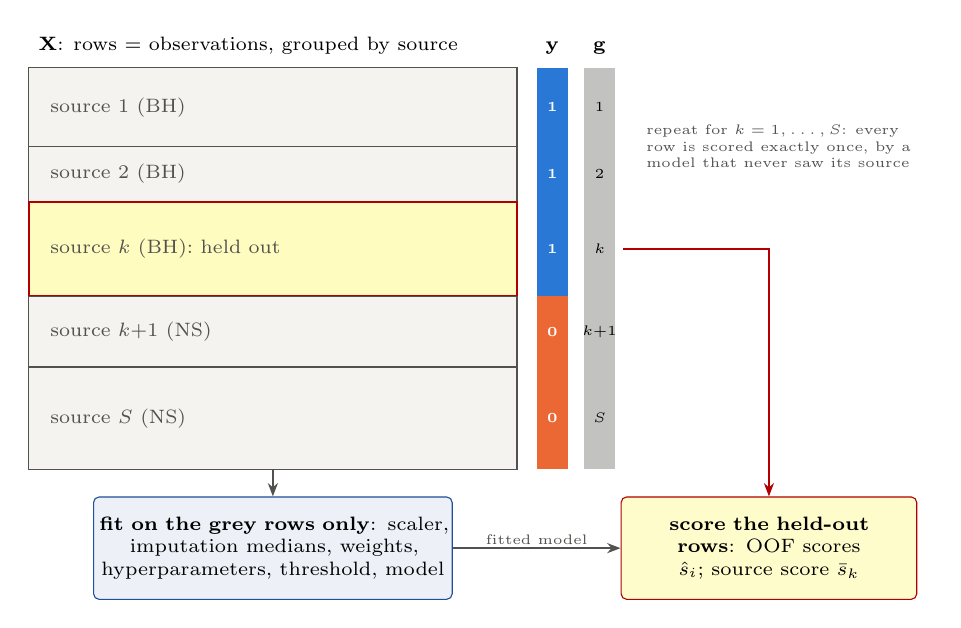
\begin{tikzpicture}[x=1cm, y=1cm, font=\scriptsize]
  \def\W{6.2}
  \foreach \yo/\h/\nm/\cl/\tst/\yy/\gg in {0/1.0/{source 1 (BH)}/bhblue/0/1/1, -1.0/0.7/{source 2 (BH)}/bhblue/0/1/2,
      -1.7/1.2/{source $k$ (BH): held out}/bhblue/1/1/k, -2.9/0.9/{source $k{+}1$ (NS)}/nsorange/0/0/{k{+}1}, -3.8/1.3/{source $S$ (NS)}/nsorange/0/0/S} {
     \ifnum\tst=1
        \fill[yellow!25] (0,\yo) rectangle (\W,\yo-\h); \draw[thick, red!70!black] (0,\yo) rectangle (\W,\yo-\h);
        \coordinate (testE) at (\W+1.35,\yo-\h/2);
     \else
        \fill[boxgrey] (0,\yo) rectangle (\W,\yo-\h); \draw[inkgrey] (0,\yo) rectangle (\W,\yo-\h);
     \fi
     \node[anchor=west, text=inkgrey] at (0.15,\yo-\h/2) {\nm};
     \fill[\cl] (\W+0.25,\yo) rectangle (\W+0.65,\yo-\h);
     \fill[inkgrey!35] (\W+0.85,\yo) rectangle (\W+1.25,\yo-\h);
     \node[white, font=\tiny\bfseries] at (\W+0.45,\yo-\h/2) {\yy};
     \node[font=\tiny] at (\W+1.05,\yo-\h/2) {$\gg$};
  }
  \node at (\W+0.45,0.25) {$\yv$}; \node at (\W+1.05,0.25) {$\gv$};
  \node[anchor=south west] at (0,0.05) {$\Xm$: rows = observations, grouped by source};
  \node[fc model, text width=4.4cm, minimum height=13mm] (fit) at (3.1,-6.1)
     {\textbf{fit on the grey rows only}: scaler, imputation medians, weights, hyperparameters, threshold, model};
  \node[fc, draw=red!70!black, fill=yellow!20, text width=3.6cm, minimum height=13mm] (pred) at (9.4,-6.1)
     {\textbf{score the held-out rows}: OOF scores $\hat s_i$; source score $\bar s_k$};
  \draw[fc arr] (3.1,-5.1) -- (fit.north);
  \draw[fc arr] (fit) -- node[fc note, above] {fitted model} (pred);
  \draw[fc arr, red!70!black] (testE) -| (pred.north);
  \node[fc note, text width=3.6cm, anchor=west] at (\W+1.6,-1.0) {repeat for $k=1,\dots,S$: every row is scored exactly once, by a model that never saw its source};
\end{tikzpicture}
\caption{One leave-one-source-out fold. The held-out block holds all observations of one source; every learned quantity
comes from the other sources.}\label{fig:loso}
\end{figure}

% -----------------------------------------------------------------------------------------------------
\subsection{Missing values}\label{sec:missing}
Spectral features are never missing: an observation that fails the quality rules is not in the sample. Timing features
can be missing, for example with fewer than 3 valid rows. For a block $T$ with training rows $\mathcal T$
(\code{v5lib.fill_missing}):
\begin{equation}
\begin{gathered}
m_\ell=\median_{i\in\mathcal T,\,T_{i\ell}\ \mathrm{finite}}T_{i\ell}\ \ (0\text{ if none}),\qquad
\tilde T_{i\ell}=\begin{cases}T_{i\ell}&\text{finite}\\m_\ell&\text{otherwise,}\end{cases}\\
\mu_i=\indic{\exists\ell:\ T_{i\ell}\ \text{not finite}}.
\end{gathered}\label{eq:fillmissing}
\end{equation}
$[\tilde T,\mu]$, with one indicator column, replaces $T$ in training and test rows. HEXTE colours use the same rule with one
indicator per colour. The CCTLR classifier needs no imputation: its timing term is set to zero for a row with a missing
value (\cref{sec:cctlr}). NICER features are never imputed, because observations that fail the NICER rules are excluded.
For the frozen external tests (v6a, v8b), the medians come from the S1 training set and are applied unchanged.

% -----------------------------------------------------------------------------------------------------
\subsection{Design matrices used by the analyses}\label{sec:matrices}
\Cref{tab:matrices} lists the main design matrices. The columns are the features defined in
\cref{sec:rxte,sec:nicermaxi}, and $m$ is a missing-value indicator.

{\small\setlength{\tabcolsep}{3.5pt}
\begin{longtable}{@{}>{\raggedright\arraybackslash}p{1.25cm} >{\raggedright\arraybackslash}p{3.6cm} >{\raggedright\arraybackslash}p{3.4cm} >{\raggedright\arraybackslash}p{7.0cm}@{}}
\caption{Main design matrices (shape $n\times p$) and their columns.}\label{tab:matrices}\\
\toprule
Round & Matrix & Shape & Columns; source of the rows \\
\midrule\endfirsthead
\toprule Round & Matrix & Shape & Columns; source of the rows \\ \midrule\endhead
\bottomrule\endfoot
v1 & $\Xm_A$, $\Xm_B$ & $120\times45$ & $A_{ij}$ or $B_{ij}$, $j=0..44$; \file{data/processed/features.npz} \\
v2 & $\Xm_A$, $\Xm_B$ & $456\times45$ & as v1; \file{data/v2/processed/features.npz} \\
 & $\Xm_H$, $\Xm_{HI}$ & $456\times2$, $456\times3$ & $h_1,h_2$ (+ $\log_{10}F$) \\
v3a & $\Xm_{H+B}$, $\Xm_{HI+A}$ & $456\times47$, $456\times48$ & colours with the full shape or intensity spectrum \\
v3b & $\Xm_{B3}$, $\Xm_{H3}$ & $456\times50$, $456\times3$ & 50-bin grid from 2.883\,keV; \file{features_3_25.npz} \\
v4b2 & $\Xm_H$, $\Xm_{H_R}$, $\Xm_R$ & $677\times\{2,2,45\}$ & S1 + v4b2 rows; R uses \code{pl2} \\
v4b1 & $\Xm_H$ \dots\ $\Xm_A$ & $7949\times\{2,3,45,45\}$ & all epoch-5 pointings; \file{data/v4b1/processed/features.npz} \\
v4b3 & $\Xm_{H+X}$ & $396\times6$ & $h_1,h_2,X_1,X_2$ + one indicator per HEXTE colour \\
v5 & $\Xm_{H+T}$, $\Xm_T$ & $456\times6$, $456\times4$ & $h_1,h_2,T_1,T_2,T_3,m$; joined from \file{timing_features.csv} \\
v6a & $\Xm_{H_R}$, $\Xm_{H_R+T}$ & train $456\times\{2,6\}$, test $341\times\{2,6\}$ & external set E; S1 medians for missing $T$ \\
v7c2, v8d & $\Xm_\mathrm{CCI}$, $\Xm_\mathrm{C2D}$, $\Xm_\mathrm{C1D}$ & $93\,461\times\{3,2,1\}$ & one row per MAXI day (BH vs NPNS, 61 sources) \\
v8b & $\Xm_{H_R}$, $\Xm_{H_R+T}$ & $379\times\{2,6\}$ & external set X, frozen S1 models; 99 hard-like rows \\
v8c & $\Xm_{H+HF}$ & $148\times5$ & $h_1,h_2,\mathrm{HF}_1,\mathrm{HF}_2,\mathrm{HF}_3$ \\
v9a & $\Xm_{H_N}$, $\Xm_{H_N+T_N}$ & $368\times\{2,5\}$ & $c_1,c_2$ (+ $T_1,T_2,T_3$); no missing values \\
v10a & as v9a & $366\times\{2,5\}$ & full files \\
v11 & as v9a & test $318\times\{2,5\}$ & new observations, frozen out-of-source models \\
v12 & as v9a & $534\times\{2,5\}$ & corrected and screened N1+N2 \\
v13 & as v9a & test $198\times\{2,5\}$ & corrected and screened N3; 74 hard-like rows \\
$\nu_c$ tests & $(\vect h,\log_{10}\nu_c)$ per hard-like obs. & -- & input of the permutation test (\cref{sec:permutation}), not a classifier \\
\end{longtable}}

% -----------------------------------------------------------------------------------------------------
\subsection{Leakage controls in the code}\label{sec:leakage}
\begin{enumerate}
\item \textbf{Folds by source.} \code{LeaveOneGroupOut} on $\gv$. The scripts assert that each test fold holds exactly one
source, that training and test sources are disjoint and that both classes are in training; the folds are saved
(\file{results/v2/fold_checks.csv}, \file{results/v2/folds_loso.csv}).
\item \textbf{The same folds across rounds.} The v2 folds are reused and asserted identical in v3a, v4a and v5, so paired
comparisons use the same test sets.
\item \textbf{Training-only preprocessing.} \code{StandardScaler} is part of the model object (\code{make_pipeline} or
\code{V4Model.fit}). Imputation medians and source-equal weights are computed from training rows only.
\item \textbf{Nested selection.} Anything that is selected (hyperparameters, representations, thresholds) is chosen by an
inner LOSO over the training sources, never on the test source (\cref{sec:nested}).
\item \textbf{Label-free residualisation.} The permutation tests regress timing on colour with a kNN that never sees labels,
leaving the source out (\cref{sec:permutation}).
\item \textbf{Frozen models.} External and new-observation tests use models, medians and rules fixed before the test data
were read. In same-source tests, each source is scored by the model fitted without it (\cref{sec:frozen}).
\item \textbf{Joins.} Feature tables are joined by observation ID. Where arrays are concatenated by position, the code
asserts that the ID orders agree.
\end{enumerate}

% =====================================================================================================
\section{Machine-learning methods}\label{sec:ml}
% =====================================================================================================

\subsection{Problem formulation and software}\label{sec:mlsetup}
Each model is a binary classifier on observations: it maps a feature vector $\vect x_i$ to a BH score
$s(\vect x_i)\in[0,1]$. The question is about \emph{sources}, so every score is produced out of fold (no model sees the
source it scores), and observation scores are averaged per source (\cref{eq:sourcescore}). All models are scikit-learn
1.8.0 estimators \citep{Pedregosa2011} (\file{requirements-lock.txt}) with the settings in \file{config.py}. They are wrapped in the pipelines of
\file{07_train_eval.py} and \file{v3lib.py}, in \code{V4Model} (\file{v4lib.py}, the eight-algorithm search) and in
\code{C2Model} (\file{v7lib.py}, MAXI). \Cref{tab:models} lists them.

\begin{table}[htbp]
\centering\small
\caption{Models and their roles. P = model of a planned primary comparison; B = baseline; D/E = descriptive or exploratory.}\label{tab:models}
\begin{tabularx}{\textwidth}{@{}>{\raggedright\arraybackslash}p{3.6cm}>{\raggedright\arraybackslash}p{3.3cm}>{\raggedright\arraybackslash}X c@{}}
\toprule
Model & Rounds & Code & Role \\
\midrule
Logistic regression (LR) & v1--v13 & \file{07}, \code{v3lib.MODELS}, \code{V4Model}, \code{C2Model} & P, B \\
Random forest (RF) & v1--v13 & as LR & P (v8d, v12b, v13a), D \\
Dummy (class prior) & v1, v2 & \file{07_train_eval.py} & B \\
ExtraTrees, HistGB, QDA, MLP & v4a & \code{V4Model} & E \\
RBF SVM & v4a, v7c2; v7c1 & \code{V4Model}, \code{C2Model}, \file{37} & E, reproduction \\
kNN classifier & v4a, v7c2, v8d; v7c1 & \code{V4Model}, \code{C2Model}, \file{37} & E, reproduction \\
Nested automatic selection & v4a & \code{v4lib.nested_fold} & P (v4) \\
CCTLR & v6c & \code{v6lib.CCTLR} & D \\
kNN regression (residualisation) & v6d, v9b--v13b & \code{v6lib.source_residuals} & inside the permutation tests \\
Frozen $\nu^\ast$ rule & v11, v13 & \file{57}, \file{63} & D \\
\bottomrule
\end{tabularx}
\end{table}

% -----------------------------------------------------------------------------------------------------
\subsection{Shared components}\label{sec:shared}
\paragraph{Standardisation.} Scale-sensitive models (LR, SVM, kNN, QDA, MLP, the colour part of CCTLR, the kNN regression)
standardise each feature with the training rows $\mathcal T$ of the current fit:
\begin{equation}
z_{i\ell}=\frac{x_{i\ell}-\mu_\ell}{\sigma_\ell},\qquad\mu_\ell=\frac1{|\mathcal T|}\sum_{i\in\mathcal T}x_{i\ell},\qquad
\sigma_\ell^2=\frac1{|\mathcal T|}\sum_{i\in\mathcal T}(x_{i\ell}-\mu_\ell)^2\quad(\sigma_\ell=0\Rightarrow1),\label{eq:scaler}
\end{equation}
and apply the same $(\mu_\ell,\sigma_\ell)$ to the test rows (\code{StandardScaler} inside the pipeline). Tree models use
the raw features.

\paragraph{Class-balanced weights.}\label{sec:weights} The main sample has 7 BH and 24 NS sources. With $n$ training rows,
$n_c$ of them in class $c$, \code{class_weight='balanced'} gives each row
\begin{equation}
w^\mathrm{bal}_i=\frac{n}{2\,n_{y_i}},\qquad\sum_{i:y_i=c}w^\mathrm{bal}_i=\frac n2.\label{eq:balanced}
\end{equation}
QDA takes no weights and uses equal priors instead. kNN corrects its output to equal priors (\cref{eq:knnprior}), and the MLP
receives $w^\mathrm{bal}$ as sample weights.

\paragraph{Source-equal weights (v4a, v4b1, v5 S3, v6 S3).} When sources contribute very different numbers of observations
(6 to 1329 per source in v4b1), balanced weights let the most-observed sources dominate. With $S_c$ training sources in
class $c$ and $n_k$ rows of source $k$ (\code{v4lib.source_equal_weights}):
\begin{equation}
w^\mathrm{src}_i=\frac{n}{2\,S_{y_i}\,n_{g_i}},\qquad\sum_{i:g_i=k}w^\mathrm{src}_i=\frac{n}{2S_c}\ (k\in c),\qquad\sum_{i:y_i=c}w^\mathrm{src}_i=\frac n2.\label{eq:sourceequal}
\end{equation}
Every source of a class then has the same total weight, and both classes sum to $n/2$, the scale of the balanced weights.
\code{class_weight} is set to \code{None} when these weights are passed. The first implementation normalised each class to 1
instead of $n/2$, which acted as a much stronger LR penalty. It was fixed after the v4a results and the affected parts were
re-run; no conclusion changed (decision log).

\paragraph{Scores.} \code{predict_proba[:,1]} for LR, RF, ExtraTrees, HistGB and QDA; the prior-corrected vote fraction for
kNN; the mean over seeds for the MLP; the logistic function of the decision value for SVM and CCTLR. Scores rank observations
and are thresholded at 0.5; they are not calibrated probabilities.

% -----------------------------------------------------------------------------------------------------
\subsection{Logistic regression}\label{sec:lr}
LR is the main model: H-LR (two colours) is the reference that every later model is compared against, and H+T-LR is the
primary model of v5, v6a, v8a/b, v9a, v10a and v11a. On standardised inputs, $s(\vect x)=\sigma(\vect w^\top\vect z+b)$
with $\sigma(u)=1/(1+e^{-u})$, and
\begin{equation}
(\hat{\vect w},\hat b)=\arg\min_{\vect w,b}\ \frac12\|\vect w\|_2^2+C\sum_{i\in\mathcal T}\omega_i\bigl[-y_i\log s(\vect x_i)-(1-y_i)\log(1-s(\vect x_i))\bigr],\label{eq:lrobj}
\end{equation}
with $C=1$, L-BFGS, at most 5000 iterations, an unpenalised intercept and $\omega_i=w^\mathrm{bal}_i$ (or $w^\mathrm{src}_i$).
With a few hundred rows and 2--6 features the penalty is weak. LR assumes log-odds that are linear in the standardised
features, so a timing feature has one slope everywhere in the colour plane. This is the motivation for CCTLR
(\cref{sec:cctlr}).

\subsection{Random forest}\label{sec:rf}
RF is the second reference model in every round, and the primary model of v8d (MAXI), v12b and v13a. It averages $B=500$
trees: $s(\vect x)=\frac1B\sum_b\hat p_b(\vect x)$, where $\hat p_b$ is the weighted BH fraction in the leaf of tree $b$. Each
tree is grown on a bootstrap sample (row weights $\omega_i$ times the bootstrap counts) with CART splits that maximise the
weighted decrease of the Gini impurity $G=1-\sum_c\pi_c^2$. At each node $m=\lfloor\sqrt p\rfloor$ features are candidates,
so with the two colours of H every split uses one randomly chosen colour, and with $p=6$ two. Trees grow until nodes are
pure or a child would have fewer than 2 rows (\code{min_samples_leaf=2}). Balanced class weights are computed once per fold,
and \code{random_state=42}. RF can follow non-monotone class regions, which matters for MAXI and for timing--colour
interactions. With fewer than 10 BH sources, however, a leaf can memorise one source.

% -----------------------------------------------------------------------------------------------------
\subsection{Further algorithms of the v4a search}\label{sec:otheralgs}
\begin{itemize}
\item \textbf{Dummy} (\code{strategy='prior'}): returns the training BH fraction and predicts the majority class. Under LOSO
the majority depends on the held-out source. In v1 (4+4 sources), holding out a BH leaves an NS majority and vice versa, so
the Dummy balanced accuracy is 0, not 0.5.
\item \textbf{ExtraTrees}: like RF but without bootstrap, and with one random threshold per candidate feature at each node.
\item \textbf{HistGradientBoosting}: an additive model on the log-odds scale; each of 200 trees is fitted to the weighted
gradients and Hessians of the log loss, with features pre-binned into at most 255 quantile bins. Learning rate 0.1, 15
leaves, at least 20 rows per leaf, no L2 term and no early stopping.
\item \textbf{RBF SVM}: \code{SVC} with balanced class weights and $K(\vect z,\vect z')=e^{-\gamma\|\vect z-\vect z'\|^2}$.
\code{gamma='scale'} gives $\gamma=1/(p\operatorname{Var}\vect Z)$; the v4a grid multiplies it by $\kappa\in\{0.3,1,3\}$.
The score is $\sigma(f(\vect z))$ of the decision value $f$. Platt scaling is not used, because it runs an internal random
cross-validation.
\item \textbf{kNN classifier}: the BH fraction $\hat p$ among the $k$ nearest standardised training rows (Euclidean,
uniform weights), corrected to equal priors with the training BH fraction $\pi$:
\begin{equation}
s(\vect x)=\frac{\hat p/\pi}{\hat p/\pi+(1-\hat p)/(1-\pi)}.\label{eq:knnprior}
\end{equation}
\item \textbf{QDA}: Gaussian classes with regularised covariances $\hat\Sigma_c=(1-r)S_c+rI$ ($r=0.1$) and equal priors.
\item \textbf{MLP}: one hidden layer of 32 ReLU units, Adam, $\alpha=10^{-3}$, balanced sample weights. Early stopping
holds out a stratified 20\% validation split and restores the best weights. Because a small MLP is unstable, the score is the
mean over seeds $\{0,\dots,4\}$ (outer fits) or $\{0,1,2\}$ (inner fits).
\end{itemize}
A planned 1D convolutional network on representation B was skipped, as declared in the plan, because \code{torch} was not
installed. Principal component analysis was never used: ``PCA'' in the code always means the Proportional Counter Array.

% -----------------------------------------------------------------------------------------------------
\subsection{Hyperparameters}\label{sec:hyper}
Except in the nested selection (\cref{sec:nested}) and the MAXI kNN and SVM, all hyperparameters are fixed in advance.
\Cref{tab:hyper} collects them.

{\small\setlength{\tabcolsep}{3pt}
\begin{longtable}{@{}>{\raggedright\arraybackslash}p{2.7cm}>{\raggedright\arraybackslash}p{6.3cm}>{\raggedright\arraybackslash}p{6.6cm}@{}}
\caption{Hyperparameters (\file{config.py}: \code{LR_PARAMS}, \code{RF_PARAMS}, \code{V4_FIXED}, \code{V4_GRID},
\code{V7_C2_*}, \code{V7_DEBEURS_*}).}\label{tab:hyper}\\
\toprule
Model & Fixed setting & Grid (where tuned) \\
\midrule\endfirsthead
\toprule Model & Fixed setting & Grid (where tuned) \\ \midrule\endhead
\bottomrule\endfoot
LR & $C=1$, L2, lbfgs, 5000 iterations, balanced & v4a: $C\in\{0.01,0.1,1,10\}$ \\
RF & 500 trees, \code{max_features='sqrt'}, leaf $\ge2$, balanced, seed 42 & v4a: leaf $\in\{1,2,5,10\}$; 200 trees inner, 500 outer \\
ExtraTrees & as RF & v4a: leaf $\in\{1,2,5,10\}$ \\
HistGB & learning rate 0.1, 200 iterations, 15 leaves, leaf $\ge20$, $\lambda=0$, no early stop, balanced, seed 42 & v4a: rate $\in\{0.05,0.1\}\times$ leaves $\in\{7,15\}$ \\
SVM (RBF) & $C=1$, $\gamma$ = \code{'scale'}, balanced & v4a: $C\in\{0.1,1,10\}\times\kappa\in\{0.3,1,3\}$; v7c2: $C\in\{0.1,1,10\}\times\gamma\in\{0.1,0.585,3\}$ \\
kNN & $k=15$, uniform, prior-corrected & v4a: $\{5,15,31\}$; v7c2, v8d: $\{5,15,24,35\}$ \\
QDA & $r=0.1$, priors $(0.5,0.5)$ & v4a: $r\in\{0.01,0.1,0.5\}$ \\
MLP & $(32,)$, $\alpha=10^{-3}$, early stopping (20\%), 500 epochs, seeds 0--4 & v4a: $\{(16,),(32,16)\}\times\alpha\in\{10^{-4},10^{-2}\}$ \\
CCTLR & Student $t$ with 4 d.o.f., scale floor 0.01, ridge $10^{-9}$ & none \\
kNN regression & $K=25$, uniform, neighbours from other sources & none \\
de Beurs reproduction & kNN $k=24$ on raw colours; SVM $C=0.655298$, $\gamma=0.585144$, Platt, one-vs-one, 3 classes & none (taken from the paper) \\
\end{longtable}}

% -----------------------------------------------------------------------------------------------------
\subsection{Model selection by nested leave-one-source-out}\label{sec:nested}
When anything is selected (algorithm, representation, hyperparameter or threshold), the selection runs inside each outer
training set, by an inner LOSO over its sources. The outer test source plays no part (\cref{fig:nested}).

\begin{figure}[htbp]
\centering
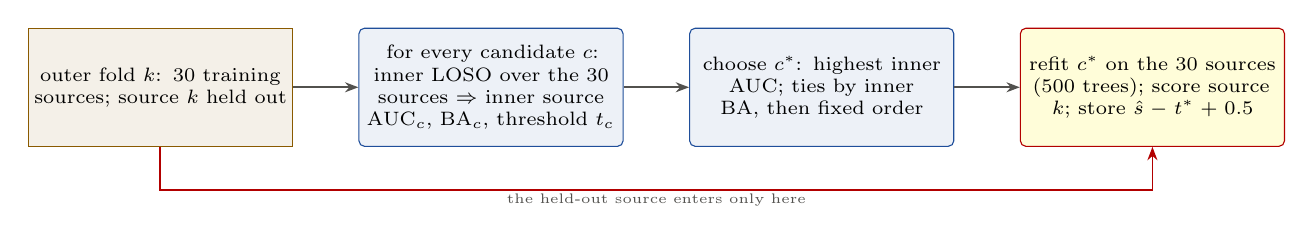
\begin{tikzpicture}[x=1cm, y=1cm,
  st/.style={fc model, text width=3.2cm, minimum height=15mm}]
  \node[fc data, text width=3.2cm, minimum height=15mm] (o) at (1.8,0) {outer fold $k$: 30 training sources; source $k$ held out};
  \node[st] (i) at (6.0,0) {for every candidate $c$: inner LOSO over the 30 sources $\Rightarrow$ inner source AUC$_c$, BA$_c$, threshold $t_c$};
  \node[st] (s) at (10.2,0) {choose $c^\ast$: highest inner AUC; ties by inner BA, then fixed order};
  \node[st, draw=red!70!black, fill=yellow!15] (f) at (14.4,0) {refit $c^\ast$ on the 30 sources (500 trees); score source $k$; store $\hat s-t^\ast+0.5$};
  \foreach \a/\b in {o/i,i/s,s/f} \draw[fc arr] (\a) -- (\b);
  \draw[fc arr, red!70!black] (o.south) -- ++(0,-0.55) -| node[fc note, pos=0.25, below] {the held-out source enters only here} (f.south);
\end{tikzpicture}
\caption{Nested LOSO (v4a). Every candidate is judged only on the outer training sources, so the cost of choosing the best
of many is included in the outer estimate.}\label{fig:nested}
\end{figure}

\paragraph{v4a (\code{v4lib.nested_fold}, \file{16_v4a_algorithms.py}).} Four representations (H, HI, B, A) are crossed with
eight algorithms and their grids (35 settings), giving 140 configurations. In part 1d, nesting runs per algorithm and
representation; in part 1e, over all 140 configurations. The inner stage uses 200 trees and MLP seeds $\{0,1,2\}$, the outer
refit 500 trees and seeds $\{0,\dots,4\}$.

\paragraph{Threshold choice (\code{v4lib.choose_threshold}).} With $u_1<\dots<u_q$ the distinct inner source scores, the
candidates are $u_1-10^{-9}$, the midpoints $(u_r+u_{r+1})/2$ and $u_q+10^{-9}$. Among those maximising the inner source
balanced accuracy, the one closest to 0.5 is taken:
\begin{equation}
t^\ast=\arg\min_{t\in\mathcal C^\ast}|t-0.5|,\qquad\mathcal C^\ast=\{t:\BA_\mathrm{src}(t)=\max_{t'}\BA_\mathrm{src}(t')\}.\label{eq:choosethreshold}
\end{equation}
The outer scores are stored shifted, $\hat s-t^\ast+0.5$, so that the common 0.5 rule applies.

\paragraph{MAXI (v7c2, v8d; \code{v7lib.c2_outer}).} kNN's $k$ is chosen by inner LOSO source AUC, and the SVM's $(C,\gamma)$
by inner \code{GroupKFold(5)} over sources (a pre-run change to save computing time). The first configuration with a strictly
higher AUC wins. Each training source contributes at most 200 randomly chosen days (seed 42), and the test source is scored
on all its days.

% -----------------------------------------------------------------------------------------------------
\subsection{Colour-conditional timing likelihood ratio (CCTLR, v6c)}\label{sec:cctlr}
In LR a timing feature has one slope everywhere, although timing is expected to help only where the colours overlap.
CCTLR adds to the H-LR logit a log-likelihood ratio of the timing features \emph{given} the colours (\code{v6lib.CCTLR}):
\begin{equation}
\ell(\vect x)=\vect w^\top\vect h+b+\sum_{k=1}^3\Bigl[\log t_4\bigl(T_k;\mu_{1k}(\vect h),\tau_{1k}\bigr)-\log t_4\bigl(T_k;\mu_{0k}(\vect h),\tau_{0k}\bigr)\Bigr],\qquad s=\sigma(\ell),\label{eq:cctlr}
\end{equation}
where $t_4$ is the Student-$t$ density with 4 degrees of freedom (robust to outliers such as bursts or dips) and
$\mu_{ck}(\vect h)=\beta_{ck0}+\beta_{ck1}h_1+\beta_{ck2}h_2$. For each class and timing band, $\vect\beta_{ck}$ is a weighted
least-squares fit on that class's rows with finite timing. The weights are $v_i=1/(S_cn_{g_i})$, so every source counts
equally, and a ridge of $10^{-9}$ is added. The scale $\tau_{ck}$ is the weighted residual standard deviation, floored at
0.01. If any timing value of a row is missing, the timing term is zero and the score equals the H-LR score. CCTLR has no
tunable parameter.

% -----------------------------------------------------------------------------------------------------
\subsection{kNN regression for colour residualisation}\label{sec:knnreg}
Inside every permutation test (\cref{sec:permutation}), the part of a timing feature $F$ (e.g.\ $\log_{10}\nu_c$) that is
predictable from colour is removed \emph{without labels} (\code{v6lib.source_residuals}). With standardised colours,
\begin{equation}
\hat F_i=\frac1K\sum_{j\in\mathcal N_K(\vect h_i;\ g_j\ne g_i)}F_j,\qquad r_i=F_i-\hat F_i,\qquad
\bar r_k=\frac1{n_k}\sum_{i:g_i=k}r_i,\label{eq:knnreg}
\end{equation}
with $K=25$ (capped at the number of available rows). The neighbours of an observation come only from \emph{other} sources,
so a source cannot explain itself. Rows with missing $F$ are skipped. If BHs cluster in one colour region, part of the class
difference is absorbed into $\hat F$, which makes the test conservative.

\subsection{Frozen characteristic-frequency rule (v11, v13)}\label{sec:nurule}
A simple rule frozen before the new data were read: a hard-like observation is called BH if $\nu_c<\nu^\ast$, and a source is
called BH if at least half of its new hard-like observations are. The threshold is the geometric mean of the class medians
in the previous data,
\begin{equation}
\nu^\ast=\sqrt{\median_\mathrm{BH}\nu_c\cdot\median_\mathrm{NS}\nu_c},\label{eq:nustar}
\end{equation}
giving 1.3007\,Hz from the v10 data (used in v11) and 1.3361\,Hz from the corrected v12 data (used in v13).
The values were written to \file{logs/v11/nu_star_frozen.txt} and \file{logs/v13/nu_star_frozen.txt} before the new
observations were read.

% -----------------------------------------------------------------------------------------------------
\subsection{Training designs}\label{sec:designs}
The same models are trained in five ways, depending on the question (\cref{tab:designs}).

\begin{table}[htbp]
\centering\small
\caption{Training designs. ``Out-of-source'': each source is scored by a model fitted on the reference data without that source.}\label{tab:designs}
\begin{tabularx}{\textwidth}{@{}>{\raggedright\arraybackslash}p{3.2cm}>{\raggedright\arraybackslash}X>{\raggedright\arraybackslash}p{4.2cm}@{}}
\toprule
Design & What is fitted and what is scored & Used in \\
\midrule
LOSO & one fit per source on all other sources; the held-out source is scored (\cref{alg:buildX}) & every development analysis (v1--v12) \\
Nested LOSO & as LOSO, plus inner LOSO selection within each training set (\cref{sec:nested}) & v4a, v7c2, v8d \\
Frozen external & one fit on S1; all external sources scored by the same model, with S1 imputation medians & v6a (set E), v8b (set X) \\
Frozen out-of-source & models fitted on the previous NICER data before the new data are read; each source's new observations are scored by the fit without that source & v11 (reference v10), v13 (reference v12) \\
All-data model & one fit on all reference data, for sources never used before & v11 (never-used sources) \\
\bottomrule
\end{tabularx}
\end{table}

% =====================================================================================================
\section{Evaluation and statistical inference}\label{sec:evaluation}
% =====================================================================================================

This section describes how a table of out-of-fold scores becomes a reported number with an interval, and how a
difference is judged. \Cref{fig:evalflow} shows the chain and \cref{tab:procedures} summarises the procedures. Every
procedure works on \emph{fixed} scores or features: nothing is refitted inside a resampling or a permutation.

\begin{figure}[htbp]
\centering
% Evaluation and inference: the chain from the design matrix to a verdict, with the version that added each tool.
% Copied from report_en/figures/flowcharts (styles in workflow_report.tex).
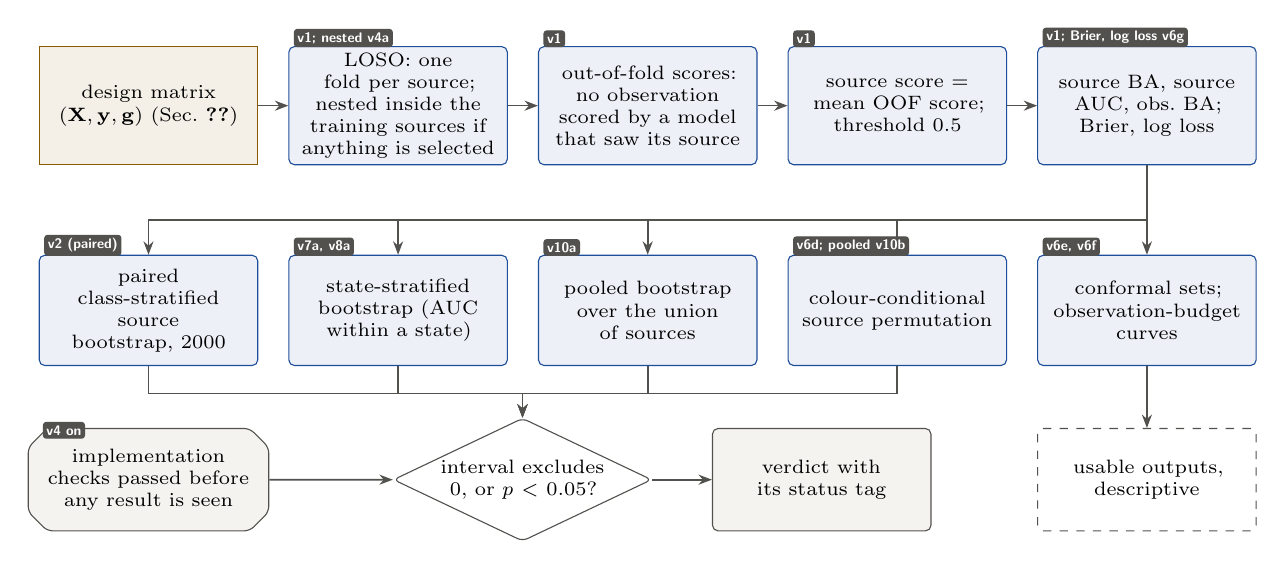
\begin{tikzpicture}[x=1cm, y=1cm,
  st/.style={fc model, text width=2.62cm, minimum height=15mm},
  inf/.style={fc model, text width=2.62cm, minimum height=14mm},
  badge/.style={fc ver, anchor=south west}]
  % row 1: from the design matrix to the metrics
  \node[fc data, text width=2.62cm, minimum height=15mm] (X) at (1.45,0) {design matrix $(\Xm,\yv,\gv)$ (Sec.~\ref{sec:datamodel})};
  \node[st] (lo) at (4.62,0) {LOSO: one fold per source; nested inside the training sources if anything is selected};
  \node[st] (oof) at (7.79,0) {out-of-fold scores: no observation scored by a model that saw its source};
  \node[st] (src) at (10.96,0) {source score = mean OOF score; threshold 0.5};
  \node[st] (met) at (14.13,0) {source BA, source AUC, obs.\ BA; Brier, log loss};
  \foreach \a/\b in {X/lo,lo/oof,oof/src,src/met} \draw[fc arr] (\a) -- (\b);
  % row 2: inference on fixed scores (no refitting)
  \node[inf] (bs) at (1.45,-2.6)  {paired class-stratified source bootstrap, 2000};
  \node[inf] (sb) at (4.62,-2.6)  {state-stratified bootstrap (AUC within a state)};
  \node[inf] (pb) at (7.79,-2.6)  {pooled bootstrap over the union of sources};
  \node[inf] (pt) at (10.96,-2.6) {colour-conditional source permutation};
  \node[inf] (cf) at (14.13,-2.6) {conformal sets; observation-budget curves};
  \coordinate (bus) at (0,-1.45);
  \draw[semithick, inkgrey] (met.south) -- (met.south |- bus);
  \draw[semithick, inkgrey] (bs.north |- bus) -- (cf.north |- bus);
  \foreach \n in {bs,sb,pb,pt,cf} \draw[fc arr] (\n.north |- bus) -- (\n.north);
  % row 3: decision and outputs
  \node[fc gate, text width=2.62cm, minimum height=13mm] (ic) at (1.45,-4.75) {implementation checks passed before any result is seen};
  \node[fc dec, text width=2.1cm, aspect=2.1] (dec) at (6.2,-4.75) {interval excludes 0, or $p<0.05$?};
  \node[fc, draw=inkgrey, fill=boxgrey, text width=2.62cm, minimum height=13mm] (vd) at (10.0,-4.75) {verdict with its status tag};
  \node[fc descr, text width=2.62cm, minimum height=13mm] (uo) at (14.13,-4.75) {usable outputs, descriptive};
  \draw[fc arr] (ic) -- (dec);
  \foreach \n in {bs,sb,pb,pt} \draw[fc arr] (\n.south) -- ++(0,-0.35) -| (dec.north);
  \draw[fc arr] (dec) -- (vd);
  \draw[fc arr] (cf) -- (uo);
  % badges: the version that introduced each element
  \foreach \n/\v in {lo/{v1; nested v4a}, oof/v1, src/v1, met/{v1; Brier, log loss v6g}, bs/{v2 (paired)}, sb/{v7a, v8a}, pb/v10a, pt/{v6d; pooled v10b}, cf/{v6e, v6f}, ic/{v4 on}}
     \node[badge] at ([xshift=2pt, yshift=-0.4pt]\n.north west) {\v};
\end{tikzpicture}

\caption{Evaluation chain from the design matrix to a verdict, with the round that introduced each element. Bootstrap and
permutation results are judged by the planned rule; conformal sets and budget curves are always descriptive.}\label{fig:evalflow}
\end{figure}

\begin{table}[htbp]
\centering\small
\caption{Inferential procedures. ``Unit'' is what is resampled or permuted.}\label{tab:procedures}
\begin{tabularx}{\textwidth}{@{}>{\raggedright\arraybackslash}p{3.5cm}>{\raggedright\arraybackslash}p{3.4cm}>{\raggedright\arraybackslash}p{2.5cm}>{\raggedright\arraybackslash}X@{}}
\toprule
Procedure & Statistic & Unit, size & Decision rule; code \\
\midrule
Class-stratified source bootstrap & source and observation BA and AUC; Brier, log loss & sources within class; 2000, seed 42 & 95\% percentile interval; a paired difference is detected if its interval excludes 0 (\code{v4lib.paired_bootstrap}) \\
State-stratified bootstrap & observation AUC within a state & sources of the whole sample; 2000 & as above (\code{v8lib.strat_boot}) \\
Pooled bootstrap (v10a) & mean of the instruments' AUC gains & union of sources; 2000 & as above (\code{v10lib.pooled_boot}) \\
Colour-conditional permutation & $D$ = BH $-$ NS mean residual & source labels; 20\,000, seed 42 & two-sided $p<0.05$; Holm across features (\code{v6lib.perm_test}, \code{holm}) \\
Pooled permutation (v10b) & mean of the instruments' $D$ & labels within membership strata; 20\,000 & $p<0.05$ (\code{v10lib.pooled_perm}) \\
Mondrian conformal sets (v6e) & per-class $p$-values & calibration sources & set $=\{y:p_y>\varepsilon\}$, $\varepsilon\in\{0.1,0.2\}$ \\
Observation budget (v6f) & source BA, AUC with $k$ observations per source & observations within a source; 500 draws & median and 2.5--97.5\% range \\
\bottomrule
\end{tabularx}
\end{table}

% -----------------------------------------------------------------------------------------------------
\subsection{Cross-validation and out-of-fold scores}\label{sec:loso}
Folds come from \code{LeaveOneGroupOut} on $\gv$ (\code{v3lib.run_loso}, \code{v4lib.loso_scores}). The OOF score of
observation $i$ is $\hat s_i=s(\vect x_i;\hat\theta^{(-g_i)})$, where $\hat\theta^{(-k)}$ is fitted, with every learned step,
on all rows of the other sources. For comparison only, v1 and v2 also ran a leaky split over observations
(\code{StratifiedKFold(5, shuffle=True, random_state=42)}), in which a source appears in both training and test; it served
only to show how optimistic such a split is.

% -----------------------------------------------------------------------------------------------------
\subsection{Metrics}\label{sec:metrics}
\begin{itemize}
\item \textbf{Balanced accuracy:} $\BA=\frac12(\mathrm{TPR}+\mathrm{TNR})$. At \emph{source level} it uses the decisions
$\hat Y_k$; with 7 BH and 24 NS sources, calling everything NS would already get 24 of 31 sources right, so BA, not
accuracy, is reported. At \emph{observation level} it uses the observation decisions; inside the bootstrap it is computed
from per-source counts of correct observations.
\item \textbf{ROC AUC} (Mann--Whitney form, ties counted as one half), for positive scores $a_r$ and negative scores $b_q$:
\begin{equation}
\AUC=\frac1{n_1n_0}\sum_{r=1}^{n_1}\sum_{q=1}^{n_0}\Bigl[\indic{a_r>b_q}+\tfrac12\indic{a_r=b_q}\Bigr].\label{eq:auc}
\end{equation}
\emph{Source AUC} uses the source scores: it is the probability that a random BH source scores above a random NS source, and
does not depend on the threshold. \emph{Observation AUC} uses all observations and is used within states.
\item \textbf{Proper scores (v6g):} class-balanced source-level log loss and Brier score, with source scores clipped to
$[0.01,0.99]$. Unlike AUC, they cannot saturate at a perfect ranking.
\end{itemize}

% -----------------------------------------------------------------------------------------------------
\subsection{Class-stratified source bootstrap}\label{sec:bootstrap}
The source is the unit of generalisation, so uncertainty is estimated by resampling sources while keeping the OOF scores
fixed. The draws are identical in every round:
\begin{enumerate}
\item the BH and NS source names are sorted, and \code{rng = numpy.random.default_rng(42)};
\item draw $b$ ($b=1,\dots,2000$) takes $S_1$ BH sources and $S_0$ NS sources with replacement,
\[
\mathcal D^{(b)}=\bigl(\mathrm{rng.choice}(\mathcal S_\mathrm{BH},S_1),\ \mathrm{rng.choice}(\mathcal S_\mathrm{NS},S_0)\bigr);
\]
\item every metric is recomputed on the drawn multiset, where a source drawn twice counts twice and brings all its
observations;
\item the 95\% interval is the percentile interval $[Q_{0.025},Q_{0.975}]$ of the 2000 values.
\end{enumerate}
\textbf{Paired differences.} Two models evaluated on the same sources use the same draws, so the difference is computed
draw by draw, $\Delta^{(b)}=M_A^{(b)}-M_B^{(b)}$. The script also stores \code{frac_first_better}, the fraction of draws with
$\Delta^{(b)}>0$. \textbf{Decision rule} (planned from v4 on): a difference is \emph{detected} only if its 95\% interval
excludes 0. An interval that touches 0 is not detected. Each metric is judged separately; source BA and source AUC are the
headline metrics. Code: \file{09_bootstrap_sources.py}, \code{v3lib.bootstrap}, \code{v4lib.paired_bootstrap},
\code{v7lib.boot_draws}.

\paragraph{What the interval contains.} Models are not refitted inside the bootstrap, so the interval reflects which sources
happen to be in the sample, not the variability of fitting or selection. With 7 BH sources, one BH source changes the source
BA by $1/14\approx0.07$, so many interval endpoints sit exactly at 0.

\paragraph{State-stratified variant (\code{v8lib.strat_boot}).} For an observation-level metric within a state, sources are
drawn from the whole sample (the same draws as above), and the metric is computed on the drawn sources' observations in that
state. A draw without BH or without NS observations in the state gives NaN and is ignored; the number of valid draws is
reported. Differences between states and between models are paired by draw.

\paragraph{Pooled variant (v10a, \code{v10lib.pooled_boot}).} RXTE and NICER sources within $0.1^\circ$ of each other are
mapped to one canonical name (\code{v10lib.canonical_map}). Draws are taken over the union of sources. In each draw each
component (RXTE development, RXTE external, NICER) computes its own state-stratified gain, and the pooled statistic is their
equal-weight mean. A source observed by two instruments is therefore drawn, or not, in both at once.

% -----------------------------------------------------------------------------------------------------
\subsection{Colour-conditional source permutation test}\label{sec:permutation}
The question is: at matched colour, does a timing feature $F$ differ between BH and NS sources? \Cref{fig:permflow} shows
the procedure.

\begin{figure}[htbp]
\centering
% Colour-conditional source permutation test (Sec. 5.6, Algorithm 3). Copied from report_en/figures/flowcharts (styles in workflow_report.tex).
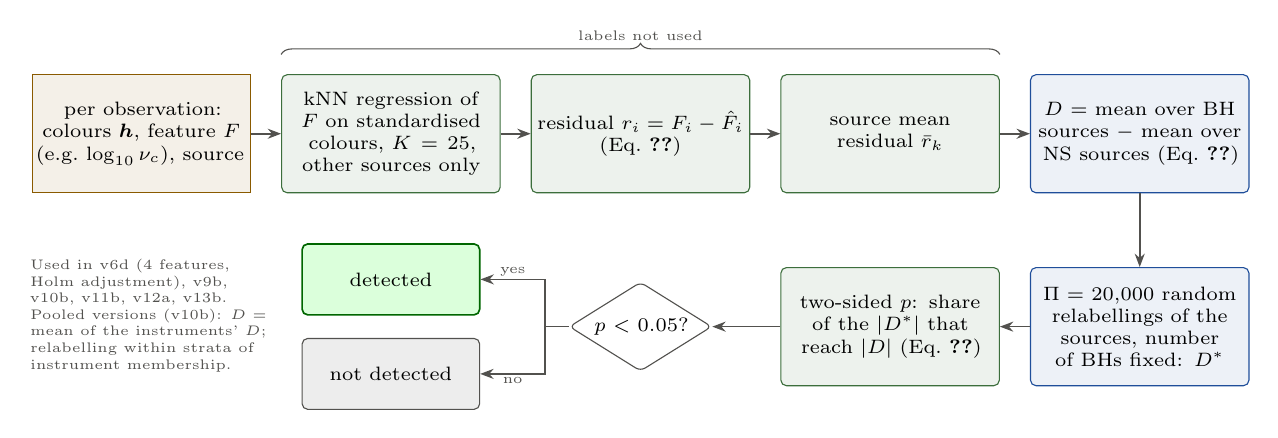
\begin{tikzpicture}[x=1cm, y=1cm,
  st/.style={fc proc, text width=2.62cm, minimum height=15mm},
  lab/.style={font=\tiny, text=inkgrey, inner sep=1pt}]
  % row 1: label-free residualisation and the statistic
  \node[fc data, text width=2.62cm, minimum height=15mm] (in) at (1.45,0) {per observation: colours $\vect h$, feature $F$ (e.g.\ $\log_{10}\nu_c$), source};
  \node[st] (kn) at (4.62,0) {kNN regression of $F$ on standardised colours, $K=25$, other sources only};
  \node[st] (rs) at (7.79,0) {residual $r_i=F_i-\hat F_i$ (Eq.~\ref{eq:knnreg})};
  \node[st] (sm) at (10.96,0) {source mean residual $\bar r_k$};
  \node[fc model, text width=2.62cm, minimum height=15mm] (D) at (14.13,0) {$D$ = mean over BH sources $-$ mean over NS sources (Eq.~\ref{eq:D})};
  \foreach \a/\b in {in/kn,kn/rs,rs/sm,sm/D} \draw[fc arr] (\a) -- (\b);
  \draw[decorate, decoration={brace, amplitude=4pt}, inkgrey] ([yshift=2.5mm]kn.north west) -- node[lab, above=4pt] {labels not used} ([yshift=2.5mm]sm.north east);
  % row 2 (right to left): null distribution, p-value, decision
  \node[fc model, text width=2.62cm, minimum height=15mm] (nl) at (14.13,-2.45) {$\Pi=20{,}000$ random relabellings of the sources, number of BHs fixed: $D^{\ast}$};
  \node[st] (pv) at (10.96,-2.45) {two-sided $p$: share of the $|D^\ast|$ that reach $|D|$ (Eq.~\ref{eq:permp})};
  \node[fc dec, text width=1.35cm, aspect=1.6] (dc) at (7.79,-2.45) {$p<0.05$?};
  \node[fc yes, text width=2.1cm, minimum height=9mm] (y) at (4.62,-1.85) {detected};
  \node[fc no, text width=2.1cm, minimum height=9mm] (n) at (4.62,-3.05) {not detected};
  \draw[fc arr] (D) -- (nl); \draw[fc arr] (nl) -- (pv); \draw[fc arr] (pv) -- (dc);
  \draw[fc arr] (dc.west) -- ++(-0.3,0) |- node[lab, pos=0.75, above] {yes} (y.east);
  \draw[fc arr] (dc.west) -- ++(-0.3,0) |- node[lab, pos=0.75, below] {no} (n.east);
  % where the test was used
  \node[fc note, text width=3.0cm, anchor=north west] at (0.0,-1.55)
     {Used in v6d (4 features, Holm adjustment), v9b, v10b, v11b, v12a, v13b. Pooled versions (v10b): $D$ = mean of the instruments' $D$; relabelling within strata of instrument membership.};
\end{tikzpicture}

\caption{Colour-conditional source permutation test. The colour dependence of the feature is removed without labels, so
the class enters only through $D$ and its permutation distribution; sources, not observations, are relabelled.}\label{fig:permflow}
\end{figure}

With the source mean residuals $\bar r_k$ of \cref{eq:knnreg}, the statistic is
\begin{equation}
D=\frac1{S_1}\sum_{k\in\mathcal S_\mathrm{BH}}\bar r_k-\frac1{S_0}\sum_{k\in\mathcal S_\mathrm{NS}}\bar r_k.\label{eq:D}
\end{equation}
If, given colour, $F$ does not depend on the class, the source labels are exchangeable. The labels are therefore reassigned
at random $\Pi=20\,000$ times, keeping the number of BH sources fixed (\code{v6lib.perm_test}, seed 42), and
\begin{equation}
p=\frac{1+\#\{\pi:|D^{\ast(\pi)}|\ge|D|-10^{-15}\}}{1+\Pi}.\label{eq:permp}
\end{equation}
Because sources are permuted as a whole, the correlation between observations of one source is respected. When several
features are tested together (v6d: $T^\ast_1$, $T^\ast_2$, $T^\ast_3$, $\log_{10}\nu_c$), Holm-adjusted $p$-values are also
reported (\code{v6lib.holm}). On synthetic data with no effect, 3.3\% of 60 tests gave $p<0.05$.

\paragraph{Pooled across instruments (v10b, v12a).} Each instrument has its own residuals and $D_\iota$; the statistic is
their mean, and each source keeps one label across instruments. The planned null permuted labels over the union of sources.
A synthetic test, run before any v10b statistic, showed that this widens the null, so labels are permuted \emph{within strata
of instrument membership} (RXTE only, NICER only, both), keeping the number of BHs per stratum fixed
(\code{v10lib.pooled_perm}). On synthetic data this gave 6.5\% of $p<0.05$ under no effect (200 sets) and power 0.98 for a
1.5\,SD shift.

% -----------------------------------------------------------------------------------------------------
\subsection{Conformal sets and observation budgets (v6e, v6f)}\label{sec:conformal}
\paragraph{Mondrian conformal sets (\code{v6lib.conformal_sets}).} For a new source with score $s$, class-wise
$p$-values are computed against calibration sources of each class:
\[
p_\mathrm{BH}(s)=\frac{1+\#\{k\in\mathrm{BH}:\bar s_k\le s\}}{1+n_\mathrm{BH}},\qquad
p_\mathrm{NS}(s)=\frac{1+\#\{k\in\mathrm{NS}:\bar s_k\ge s\}}{1+n_\mathrm{NS}},
\]
and the prediction set is $\{y:p_y(s)>\varepsilon\}$ for $\varepsilon\in\{0.1,0.2\}$. The set can be $\{\mathrm{BH}\}$,
$\{\mathrm{NS}\}$, both (``cannot tell'') or empty. Two versions are used: a LOSO version on S1 (the other sources' OOF
scores calibrate) and a split version for the external set E (the S1 OOF scores calibrate the frozen-model scores).

\paragraph{Observation budget (\code{v6lib.budget_curves}).} For $k\in\{1,2,3,5,8,13,21\}$ and 500 draws (seed 42), each
source's score is the mean OOF score of $\min(k,n_k)$ of its observations, drawn without replacement, using the S3 scores
(up to 1329 observations per source). The curves show source BA and AUC against $k$.

\paragraph{Agreement and reliability.} The agreement between two models is the Spearman correlation of their OOF scores and
the fraction of identical decisions. The bridge check of v4b2 allowed H$_R$ to replace H only if the paired intervals
contained 0 and the scores correlated at Spearman $\ge0.90$. For split-half reliability, a feature is computed from odd and
even rows or segments separately, and the correlation is stepped up with Spearman--Brown, $2\rho/(1+\rho)$.

% -----------------------------------------------------------------------------------------------------
\subsection{Frozen and prospective tests}\label{sec:frozen}
For the external and new-observation tests, everything that could adapt to the test data was fixed and committed before the
data were read (\cref{fig:frozenflow,tab:frozen}). Two kinds of independence are distinguished:
\begin{itemize}
\item \emph{source-level}: the test sources were never used in training (v6a, v8b);
\item \emph{observation-level}: new observations of sources already used (v11, v13).
\end{itemize}
For NICER BHs only the second was possible, because every dynamically confirmed BH with usable timing data had already been
used.

\begin{figure}[htbp]
\centering
% Frozen and prospective protocol (Sec. 5.10, Table 5.3). Copied from report_en/figures/flowcharts (styles in workflow_report.tex).
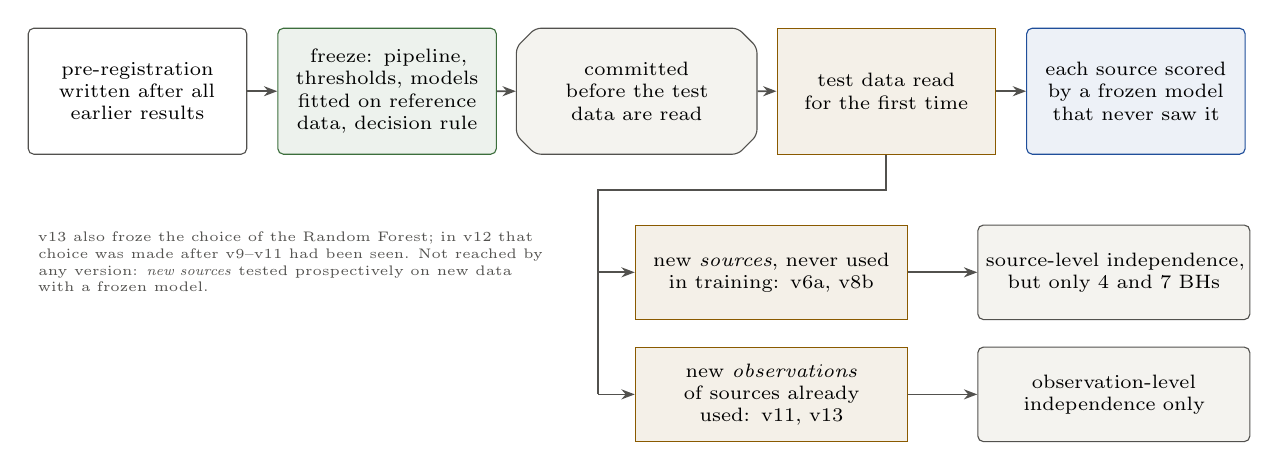
\begin{tikzpicture}[x=1cm, y=1cm,
  st/.style={fc proc, text width=2.62cm, minimum height=16mm},
  lab/.style={font=\tiny, text=inkgrey, inner sep=1pt}]
  % row 1: what happens before any test data are read
  \node[fc, draw=inkgrey, fill=white, text width=2.62cm, minimum height=16mm] (pr) at (1.45,0) {pre-registration written after all earlier results};
  \node[st] (fz) at (4.62,0) {freeze: pipeline, thresholds, models fitted on reference data, decision rule};
  \node[fc gate, text width=2.62cm, minimum height=16mm] (cm) at (7.79,0) {committed before the test data are read};
  \node[fc data, text width=2.62cm, minimum height=16mm] (nw) at (10.96,0) {test data read for the first time};
  \node[fc model, text width=2.62cm, minimum height=16mm] (os) at (14.13,0) {each source scored by a frozen model that never saw it};
  \foreach \a/\b in {pr/fz,fz/cm,cm/nw,nw/os} \draw[fc arr] (\a) -- (\b);
  % row 2: the two kinds of test data and their independence
  \node[fc data, text width=3.3cm, minimum height=12mm] (ns) at (9.5,-2.3) {new \emph{sources}, never used in training: v6a, v8b};
  \node[fc data, text width=3.3cm, minimum height=12mm] (no) at (9.5,-3.85) {new \emph{observations} of sources already used: v11, v13};
  \node[fc, draw=inkgrey, fill=boxgrey, text width=3.3cm, minimum height=12mm] (si) at (13.85,-2.3) {source-level independence, but only 4 and 7 BHs};
  \node[fc, draw=inkgrey, fill=boxgrey, text width=3.3cm, minimum height=12mm] (oi) at (13.85,-3.85) {observation-level independence only};
  \draw[semithick, inkgrey] (nw.south) -- ++(0,-0.45) -| (7.3,-3.85);
  \draw[fc arr] (7.3,-2.3) -- (ns.west); \draw[fc arr] (7.3,-3.85) -- (no.west);
  \draw[fc arr] (ns) -- (si); \draw[fc arr] (no) -- (oi);
  \node[fc note, text width=6.4cm, anchor=north west] at (0.15,-1.75)
     {v13 also froze the choice of the Random Forest; in v12 that choice was made after v9--v11 had been seen.
      Not reached by any version: \emph{new sources} tested prospectively on new data with a frozen model.};
\end{tikzpicture}

\caption{Frozen and prospective protocol.}\label{fig:frozenflow}
\end{figure}

\begin{table}[htbp]
\centering\small
\caption{What was frozen, and when (commit of the plan).}\label{tab:frozen}
\begin{tabularx}{\textwidth}{@{}>{\raggedright\arraybackslash}p{1.1cm}>{\raggedright\arraybackslash}X>{\raggedright\arraybackslash}p{4.0cm}>{\raggedright\arraybackslash}p{2.9cm}@{}}
\toprule
Test & Frozen before the test data were read & How the models are applied & Record \\
\midrule
v6a & H$_R$-LR, H$_R$+T-LR and CCTLR(H$_R$) fitted once on S1; imputation medians from S1 & every external source scored by the same S1 models & plan v6 \\
v8b & the v6 models; the v7a state rule & external set X & plan v8 (\texttt{a481fa0}) \\
v11 & NICER feature pipeline, state thresholds, models fitted on the v10 data, $\nu^\ast=1.3007$\,Hz & out-of-source for the v9 sources; all-data model for never-used sources & plan \texttt{6fea016}; $\nu^\ast$ \texttt{58ded89} \\
v13 & v12 pipeline with 3C50 correction and screening, RF as the primary model, models fitted on the 534 v12 observations, $\nu^\ast=1.3361$\,Hz & out-of-source & plan \texttt{42fe1d2} \\
\bottomrule
\end{tabularx}
\end{table}

% -----------------------------------------------------------------------------------------------------
\subsection{Implementation checks and how verdicts are labelled}\label{sec:ic}
From v4 on, every round defines \emph{implementation checks} (IC) that must pass before any result is looked at. Examples:
\begin{itemize}
\item earlier OOF predictions are reproduced to $10^{-8}$--$10^{-15}$;
\item synthetic signals are recovered by the timing estimators within 10\%;
\item pure-Poisson data give $|z|<3$;
\item known sources behave as expected (XTE J1118+480 hard-like, Z sources soft-like);
\item results agree with independent tools (XSPEC, \code{astropy}).
\end{itemize}
The unit tests are \file{scripts/test_v4lib.py}--\file{test_v11lib.py}, and their logs are in \file{logs/}. A failed check
stops the sub-analysis (the scripts exit with code 3) or downgrades it to exploratory.

Each sub-analysis declares one \emph{primary} comparison in its plan; the others are \emph{secondary} or \emph{descriptive}
and are not used to claim a difference. Comparisons added after results were seen are labelled \emph{post hoc}. No
family-wise correction is applied across descriptive comparisons; where there are many (v4a: 76 combinations $\times$ 3
metrics), the reports state how many intervals would exclude 0 by chance and draw no conclusion from them. Within the v6d
permutation family, Holm adjustment is reported.

% =====================================================================================================
\section{Running, logging and reproducing the workflow}\label{sec:operations}
% =====================================================================================================

\subsection{Software environment}\label{sec:env}
\begin{itemize}
\item \textbf{Python.} Python 3.12.10 in a virtual environment on Windows (\file{logs/environment.txt}); the re-checks used
macOS with Python 3.12.14. Packages are pinned in \file{requirements-lock.txt}, among them numpy 2.4.4, pandas 2.3.3,
scipy 1.17.1, scikit-learn 1.8.0, astropy 7.2.0, matplotlib 3.10.9, joblib 1.6.0 and requests 2.33.1.
\item \textbf{HEASoft.} HEASoft 6.37.1 runs in WSL Ubuntu 22.04, in a conda environment \code{henv} created by
\file{scripts/install_heasoft_wsl.sh} (Miniforge, then \code{mamba create -n henv heasoft} from the HEASARC conda channel).
It is called from Python with \code{wsl -d Ubuntu-22.04 -u root -- bash <script>} in three places only: the XSPEC
cross-check (v2), \code{nh} and XSPEC \code{tbabs} (v8d), and \code{nibackgen3C50} with the NICER CALDB (v12, v13). On Linux
the two shell scripts can be run directly.
\item \textbf{Other tools.} \code{curl} for range requests (NICER, RXTE event files) and for downloads inside WSL.
\end{itemize}

\subsection{Environment variables}\label{sec:envvars}
\begin{center}\small
\begin{tabularx}{\textwidth}{@{}l >{\raggedright\arraybackslash}X@{}}
\toprule
Variable & Effect \\
\midrule
\code{XRB_VERSION} & selects the \file{config.py} block and the output folders (\code{v1} if unset); most scripts set it themselves \\
\code{XRB_PY} & Python interpreter used by the run scripts (default \file{~/venvs/xrb-pilot/bin/python}) \\
\code{XRB_EXTERNAL_RAW} & folder for large raw data outside the repository (default \file{~/xrb-pilot-data/raw}) \\
\code{V4_JOBS} & parallel jobs of the v4a search (default 16) \\
\code{V7C_SMOKE}, \code{V9_SMOKE} & quick test runs on a few sources or groups (outputs written to \file{*_smoke.csv}) \\
\code{V9_THREADS} & parallel (source, group) pairs in the v9 NICER fetch (default 8) \\
\code{V8_SKIP_HF} & skip the event-mode part of \file{44_v8_analysis.py} \\
\bottomrule
\end{tabularx}
\end{center}

\subsection{Run scripts and order}\label{sec:runorder}
Each round has a Bash and a PowerShell driver in the repository root. They run the unit tests first, then the scripts in
order, writing one log per script to \file{logs/<v>/}. \Cref{tab:runs} gives the order. Rounds build on each other, so they
must be run in sequence; downloads are cached, so a re-run fetches only what is missing.

{\small\setlength{\tabcolsep}{3pt}
\begin{longtable}{@{}>{\raggedright\arraybackslash}p{2.5cm}>{\raggedright\arraybackslash}p{9.0cm}>{\raggedright\arraybackslash}p{4.1cm}@{}}
\caption{Run scripts (\file{.sh}; the \file{.ps1} versions are equivalent) and the scripts they call, in order.}\label{tab:runs}\\
\toprule
Driver & Scripts called & Notes \\
\midrule\endfirsthead
\toprule Driver & Scripts called & Notes \\ \midrule\endhead
\bottomrule\endfoot
\file{run_all.sh} & 03, 04, 05 (v1 only), 06, 07, 08, 09; 10 with \code{--xspec} & \code{--v2} switches to v2 \\
\file{run_v3.sh a b c} & a: 11; b: 12; c: 13, then 03/04/06 with \code{XRB_VERSION=v3c}, then 14 & verify the candidate list first \\
\file{run_v4.sh test a burst b3 b2 b1} & test\_v4lib; a: 16; burst: 17, 18; b3: 19; b2: 20, 21, 22; b1: 23, 24, 25 & b1 downloads about 2\,GB \\
\file{run_v5.sh} & test\_v5lib, 26, 27 & 26 stops if a check fails \\
\file{run_v6.sh} & test\_v6lib, 28, 21 (\code{XRB_VERSION=v6}), 29, 30 & \\
\file{run_v7.sh} & test\_v7lib, 31, 32, 33, 34, 35, 04 (\code{v7b2}), 31 \code{--sample v7b2}, 36, 37, 38, 39, 40 & 39 takes about 2\,h \\
\file{run_v8.sh} & test\_v8lib, 41, 21 (\code{v8b}), 42, 43, 44, 45, 46 & 45 needs HEASoft (WSL) \\
\file{run_v9.sh} & test\_v9lib, 47, 48, 49, 50, 51 & prefixes about 14\,GB \\
\file{run_v10.sh} & test\_v10lib, 52, 53, 54 & tails about 24\,GB \\
\file{run_v11.sh} & test\_v11lib, 55, 56, 57 & streams about 40\,GB, not stored \\
\file{run_v12.sh} & 58, 59 & 3C50 through WSL \\
\file{run_v13.sh} & 60, 61, 62, 63 & \\
\end{longtable}}

\paragraph{Stops.} A script exits with code 3 when a planned check fails: implementation checks (26, 43, 44, 45), the
Z-source and XTE J1118+480 sanity gates (34, 49, 59, 63), the reproduction tolerance (37) and the overlap checks of the
NICER selections (55, 60). The drivers stop at that point, except after 43: the recorded v8c run failed its check, so v8c is
exploratory and the driver continues.

\subsection{Logs and checkpoints}\label{sec:logs}
\begin{itemize}
\item \file{logs/<v>/<script>.log}: the standard output of each script, with counts, statuses and timings.
\item \file{logs/progress.jsonl} and \file{reports/progress.json}: one entry per completed stage (\code{common.progress}).
\item \file{logs/downloads.jsonl}: the download log of \cref{sec:provenance}. It has 50\,777 lines: 50\,773 JSON records,
three fragments of interrupted concurrent writes and one empty line.
\item \file{logs/04_errors.log}: tracebacks of RXTE candidates that could not be fetched or read.
\item \file{data/v11/observations_partial.jsonl}, \file{data/v13/observations_partial.jsonl},
\file{data/v12/bkg3c50_partial.jsonl}, \file{data/v13/bkg3c50_partial.jsonl}: checkpoints of the long NICER steps; an
interrupted run resumes from them.
\item \file{logs/v11/nu_star_frozen.txt}, \file{logs/v13/nu_star_frozen.txt}: the frozen $\nu^\ast$ values.
\end{itemize}

\subsection{Plans, decision log and branches}\label{sec:plans}
\begin{itemize}
\item \textbf{Plans.} \file{reports/preregistration.md} (v1) and \file{reports/preregistration_v2.md} to \file{_v13.md}.
Each is a time-stamped, internally pre-specified analysis plan, written after all earlier results and before the round's data
were downloaded. It fixes the samples, features, models, primary comparison and decision rule. The matching block of
\file{config.py} is committed with it.
\item \textbf{Decision log.} \file{reports/decision_log.md} records every deviation, bug fix and added comparison, with the
time and whether it was made after the round's results were seen.
\item \textbf{Branches.} From v3 on, each round was developed on a branch \file{vN-analysis} and merged into
\file{master} through a pull request (v3 to v13, then a v14 wrap-up). The commit SHAs of the frozen plans are cited in
\cref{tab:frozen}.
\item \textbf{Reports.} Each round has a report \file{reports/report_vN_zh-TW.md}, ending with a ``re-run'' section that
lists the exact order, durations and download volumes.
\end{itemize}

\subsection{Data locations}\label{sec:locations}
\begin{itemize}
\item \textbf{In git:} source tables; candidate tables; every tried observation with its status and reason
(\file{data/*/observations.csv}); processed features (\file{features.npz}, \file{*_features.csv}); out-of-fold predictions;
result tables (\file{results/}); figures; logs.
\item \textbf{Not in git} (\file{.gitignore}): raw RXTE products of v1--v3 and the v8 event files in \file{data/raw/}; under
\code{XRB_EXTERNAL_RAW}, the v4b1 files, the NICER prefixes (v9), tails (v10) and the v13 cleaned files of faint
observations; the 3C50 spectra in \file{~/xrb-pilot-data/nicer_bkg_spectra/}; the NICER CALDB in
\file{~/xrb-pilot-data/caldb/}. Everything can be fetched again with the scripts.
\end{itemize}

\subsection{How to reproduce a result}\label{sec:reproduce}
\begin{enumerate}
\item Clone the repository, create a Python 3.12 virtual environment and run \code{pip install -r requirements-lock.txt}.
\item For v2 (XSPEC), v8d, v12 and v13, install HEASoft in WSL with \file{scripts/install_heasoft_wsl.sh}, and for v12--v13
unpack the NICER CALDB into \file{~/xrb-pilot-data/caldb}.
\item Run the drivers in order (\cref{tab:runs}). Each script re-downloads only missing files, re-applies the frozen rules
and rewrites its outputs.
\item Compare: re-downloaded files can be checked against the SHA256 values in \file{logs/downloads.jsonl}, and the
regenerated tables against the committed ones (\code{git diff}).
\end{enumerate}
This was done once in full for v1--v2 on a second machine (macOS). All 2\,689 raw files matched their SHA256 values.
\file{features.npz} agreed to $\le10^{-16}$, LR scores were identical, single RF scores differed by at most 0.006 (source means
by at most 0.001), and all predicted labels and accuracies were identical.

\subsection{Script index}\label{sec:scripts}
{\footnotesize\setlength{\tabcolsep}{3pt}
\begin{longtable}{@{}>{\raggedright\arraybackslash}p{3.6cm}>{\raggedright\arraybackslash}p{5.6cm}>{\raggedright\arraybackslash}p{6.4cm}@{}}
\caption{Analysis scripts (\file{scripts/}), what they do and their main outputs.}\label{tab:scriptmap}\\
\toprule
Script & Purpose & Main outputs \\
\midrule\endfirsthead
\toprule Script & Purpose & Main outputs \\ \midrule\endhead
\bottomrule\endfoot
\file{01}, \file{02} & inspect the archive; download MissionLongData catalogues & \file{data/cache/}, \file{data/raw/catalogs/} (not in git) \\
\file{03_select_observations.py} & source table and time-stratified candidates & \file{sources.csv}, \file{observation_candidates.csv}, \file{attrition_catalog.csv} \\
\file{04_fetch_process.py} & download Standard Products, dead time, quality rules, rebinning & \file{features.npz}, \file{observations.csv}, \file{attrition_download.csv} \\
\file{05}, \file{06} & two-source data-flow check; dataset checks & \file{reports/step2_fits_check.md}, \file{results/data_checks.md} \\
\file{07}, \file{08}, \file{09} & LOSO (Dummy, LR, RF) and leaky split; error analysis; source bootstrap & \file{oof_predictions_loso.csv}, \file{folds_loso.csv}, \file{bootstrap_source_level.csv} \\
\file{10_xspec_crosscheck.py} & XSPEC check of the background subtraction (WSL) & \file{results/v2/xspec_crosscheck.csv} \\
\file{11}, \file{12} & v3a increments; v3b 3--25\,keV & \file{results/v3/} \\
\file{13}, \file{14} & v3c candidate catalogues and scores & \file{data/v3c/}, \file{results/v3c/} \\
\file{15} & colour--colour summary figure & \file{figures/final/} \\
\file{16_v4a_algorithms.py} & eight-algorithm search, nested selection & \file{results/v4/v4a_*} \\
\file{17}, \file{18} & burst detection; burst exclusion & \file{results/v4/burst_*} \\
\file{19_v4b3_hexte.py} & HEXTE colours & \file{data/v4b3/processed/hexte_features.csv} \\
\file{20}--\file{22} & v4b2: position-matched sources, download, analysis & \file{data/v4b2/}, \file{results/v4b2/} \\
\file{23}--\file{25} & v4b1: all epoch-5 pointings & \file{data/v4b1/}, \file{results/v4b1/} \\
\file{26}, \file{27} & Standard-1 timing features; v5 analysis & \file{data/v5/processed/timing_features.csv}, \file{results/v5/} \\
\file{28}--\file{30} & external sources; all-pairs timing and $\nu_c$; v6a--h & \file{data/v6/}, \file{results/v6/} \\
\file{31}--\file{33} & MINBAR matching, replacement, exclusion & \file{results/v7b1/}, \file{data/v7b1/} \\
\file{34_v7a_states.py} & variability states & \file{results/v7a/states.csv} \\
\file{35}, \file{36} & persistent BHs & \file{data/v7b2/}, \file{results/v7b2/} \\
\file{37_v7c1_repro.py} & reproduction of de Beurs et al. & \file{results/v7c/v7c1_*} \\
\file{38}, \file{39} & MAXI selection, cuts and models & \file{data/v7c/}, \file{results/v7c/v7c2_*} \\
\file{41}, \file{42} & new BHs; states and timing of the external set & \file{data/v8b/} \\
\file{43_v8c_events.py} & event-mode features & \file{data/v8c/processed/hf_features.csv} \\
\file{44}, \file{45} & v8a--c analysis; $N_\mathrm{H}$ correction (WSL) & \file{results/v8*/}, \file{data/v8d/} \\
\file{47}--\file{49} & NICER selection, prefix features, analysis & \file{data/v9/}, \file{results/v9a/}, \file{results/v9b/} \\
\file{50} & MAXI colour strata & \file{results/v9c/} \\
\file{52}--\file{54} & NICER full files; RXTE $\nu_c$ table; pooled tests & \file{data/v10/}, \file{results/v10a/}--\file{v10c/} \\
\file{55}--\file{57} & new NICER observations; frozen tests & \file{data/v11/}, \file{results/v11/} \\
\file{58}, \file{59} & 3C50 (WSL); corrected analysis & \file{data/v12/}, \file{results/v12/} \\
\file{60}--\file{63} & third NICER set; frozen v12 pipeline & \file{data/v13/}, \file{results/v13/} \\
\file{40}, \file{46}, \file{51}, \file{64} & summary figures & \file{figures/v7/}, \file{figures/v8/}, \file{figures/v9/}, \file{figures/final/} \\
\file{common.py}, \file{spectra.py}, \file{config.py}, \file{plotstyle.py} & download and progress log; Standard-2 reader; settings; plot style & -- \\
\file{v3lib.py}--\file{v11lib.py} & round libraries (representations, models, bootstrap, timing, NICER) & -- \\
\file{test_v4lib.py}--\file{test_v11lib.py} & implementation checks on synthetic data & \file{logs/v*/test_*.log} \\
\file{v12_bkg3c50.sh}, \file{v8d_heasoft.sh}, \file{install_heasoft_wsl.sh} & HEASoft steps in WSL & -- \\
\end{longtable}}


\appendix
% =====================================================================================================
\section{File schemas}\label{app:schemas}
% =====================================================================================================

The columns below were read from the committed files at commit \texttt{666c2e0}. ``Rows'' is the row count of the example
file named. Files of other rounds with the same name have the same columns, unless noted.

{\small\setlength{\tabcolsep}{3pt}
\begin{longtable}{@{}>{\raggedright\arraybackslash}p{4.4cm}>{\raggedright\arraybackslash}p{11.2cm}@{}}
\caption{Schemas of the main tables and arrays.}\label{tab:schemas}\\
\toprule
File (example; rows) & Columns and meaning \\
\midrule\endfirsthead
\toprule File (example; rows) & Columns and meaning \\ \midrule\endhead
\bottomrule\endfoot
\multicolumn{2}{@{}l}{\emph{RXTE}}\\
\file{data/v2/sources.csv} (33) & \code{source_id, name, aliases, ra_deg, dec_deg, label, evidence, reference_url, status,
coord_origin, n_eligible, included}. \code{label} is BH or NS; \code{evidence} and \code{reference_url} give the labelling
evidence; \code{included} is False if fewer than the minimum number of eligible pointings remain. \\
\file{results/v2/attrition_catalog.csv} (33) & \code{source_id, catalog_rows, after_dedup, after_epoch5_window,
after_exposure, after_std1rate, after_pointing}: rows left after each eligibility step. \\
\file{data/v2/observation_candidates.csv} (7\,975) & \code{obs_id, source_id, label, time_bin, rank_in_bin, mjd,
cat_exposure, cat_npcu, cat_std1rate, pointing_sep_deg}: every eligible pointing with its time group and rank. \\
\file{data/v2/observations.csv} (462) & \emph{Candidate:} \code{obs_id, source_id, label, time_bin, rank_in_bin, mjd,
cat_exposure, cat_npcu, cat_std1rate}. \emph{Files:} \code{url_base, path_src, path_bkg, path_rsp}. \emph{Header:}
\code{date_obs, obs_mjd_start, exposure_s, bkg_exposure_s, pcus, npcu, n_gti, object_hdr, hdr_sep_deg, src_unit,
src_class, bkg_class, poisserr, sys_err, backscal_ratio, rsp_detnam, gain_shift_channels}. \emph{Dead time:} \code{dtf,
dcor, dtf_xe, dtf_std1, dtf_std1_vle150us, std1_npcu_on, std1_covered_s, std1_vle_rate_per_pcu, deadtime_method}.
\emph{Summary:} \code{net_rate_5_25, net_rate_err, net_snr, src_rate_5_25, bkg_rate_5_25, bkg_fraction,
hardness_10_25_over_5_10, n_nonpositive_bins}. \emph{Decision:} \code{status} (accepted or excluded), \code{reason},
\code{in_dataset}. \\
\file{results/v2/attrition_download.csv} (31) & \code{source_id, candidates_tried, accepted, bins_empty}. \\
\file{data/v2/processed/features.npz} (456) & \code{rate, err, srate, brate, pl2}: $456\times45$ float64 in
c\,s$^{-1}$\,keV$^{-1}$\,PCU$^{-1}$ (net rate, its error, total rate, background rate, folded $\Gamma=2$ power law);
\code{edges}: 46 grid edges in keV; \code{obs_id}, \code{source_id}: strings; \code{y}: int64 (1 = BH); \code{F}: net
5--25\,keV rate per PCU. Rows are in the order of the accepted observations. \\
\file{data/v5/processed/timing_features.csv} (8\,170) & \code{obs_id, source_id, label, bkg_rate_per_pcu, n_rows_in_gti,
n_std1_files, n_rows_valid, f_T1..f_T3} (fractional variances), \code{fauto_T1..fauto_T3} (auto-power check), \code{n_on,
src_rate_per_pcu, tot_rate_per_pcu, T1, T2, T3, T_total} (signed rms), \code{T1_auto..T3_auto, status, in_v2, in_v4b2,
in_v4b1}. \\
\file{data/v6/processed/timing_v6.csv} (8\,350) & \code{obs_id, source_id, label, n_rows_in_gti, n_rows_valid,
n_rows_pairs, n_rows_single, T1s, T2s, T3s, Ts_total, nu_c, lb0..lb8} (log-bin variances), odd/even halves
\code{T1s_odd..T3_v5_even}, \code{status, in_v2, in_v4b2, in_v4b1, in_v6}. \\
\file{results/v7a/states.csv} (456) & \code{obs_id, source_id, label, n_rows_in_gti, n_rows_burst_removed, n_rows_used, rms,
state, c1, c2}. \\
\file{data/v4b3/processed/hexte_features.csv} (456) & \code{obs_id, source_id, label, mjd, status, reason, respfile,
ancrfile, deadapp, exposure_src, exposure_bkg, X_25_40, X_25_40_err, X_40_60, X_40_60_err, nchan, F_PCA_16_25,
F_PCA_16_25_err, X1, X2, X1_den_snr, X2_den_snr}. \\
\file{data/v8c/processed/hf_features.csv} (311) & \code{obs_id, source_id, label, sample, role, bkg_rate_per_pcu,
n_event_files, n_events, n_seg}; for each band LC, HF1, HF2, HF3, NULL: \code{<band>_var, <band>_se, <band>} and the
mean-of-ratios variants; \code{NULL_z, HF1_z..HF3_z, mean_n_on, src_rate_per_pcu, tot_rate_per_pcu, exposure_s, status,
n_burst_intervals}. \\
\multicolumn{2}{@{}l}{\emph{NICER}}\\
\file{data/v9/sources.csv} (140) & \code{name, label, ra, dec, evidence, pos_origin, excluded_confused, eligible,
included}. \\
\file{data/v9/observation_candidates.csv} (3\,848) & \code{obsid, source, label, time_bin, rank_in_bin, mjd, exposure,
num_fpm, ym, url} (\code{ym} is the archive month folder). v11 and v13 add \code{group}. \\
\file{data/v11/observations.csv} (588) & \emph{Candidate:} \code{obsid, source, label, group, time_bin, rank_in_bin, mjd,
exposure_cat}. \emph{Reading:} \code{n_events, bytes, file_bytes, read_complete, sha256, url}. \emph{Segments:}
\code{n_bursts, n_seg, n_seg_burst_removed, good_time_s, rate_2_10, mean_n_mpu}. \emph{Colours:} \code{cA, cB, cC, c1,
c2}. \emph{Timing:} \code{T1_var, T1_se, T1} and the same for \code{T2, T3, STATE, WHITE}; \code{rms_nuc_band, nu_c,
lb0..lb12, lb0_se..lb12_se}. \emph{Decision:} \code{state, status} (ok, missing or excluded with reason),
\code{bkg_ratio_12_15}. The v9 file has \code{url, bytes, file_bytes, stop, rows_read} instead of the streaming
fields, and no \code{group}, \code{bkg_ratio_12_15} or \code{lb*_se}. \\
\file{data/v12/processed/bkg3c50.csv} (503) & \code{obsid, source, label, sample, rate_2_10, rc} (exit code),
\code{T_A, T_B, T_C, T_T} (total band rates), \code{B_A, B_B, B_C, B_T} (background band rates), \code{f_A, f_B, f_C, f_T}
(fractions), \code{exposure_3c50, status}. \\
\file{data/v12/processed/nicer_corrected_screened.csv} (534) & \code{obsid, source, label, c1, c2, cA, cB, cC, T1, T2, T3,
STATE, nu_c, rate_2_10, state} (after correction), \code{sample} (v10 or v11), \code{bkg_status, T_T, f_A, f_B, f_C, f_T,
f_used}. \\
\multicolumn{2}{@{}l}{\emph{MAXI}}\\
\file{data/v7c/c2_sources.csv} (134) & \code{name, cls} (BH, NPNS, PSR), \code{maxi_id, maxi_name, n_points_raw,
n_points_cut, included, evidence, match_sep_deg}. \\
\file{data/v7c/maxi_points.csv} (132\,057) & \code{mjd, f, e} (total), \code{L, eL, M, eM, H, eH} (2--4, 4--10,
10--20\,keV and errors), \code{source} (MAXI J-identifier), \code{name, cls}. \\
\file{data/v8d/nh_hi4pi.csv} (100); \file{tbabs_transmission.csv} (201) & \code{name, ra, dec, avnh, avwnh, map};
\code{nh_1e22, L, M, H} (photon flux per band for each $N_\mathrm{H}$ of the grid). \\
\multicolumn{2}{@{}l}{\emph{Model outputs}}\\
\file{results/v2/oof_predictions_loso.csv} (5\,472) & \code{representation, model, fold, source_id, obs_id, true_label,
BH_score, predicted_label}: one row per observation and model. \\
\file{results/v13/v13_frozen_predictions.csv} (792) & as the OOF table plus \code{raw_score, threshold, name, state, nu_c,
f_used}. \\
\file{results/v13/v13a_gain.csv} (21) & \code{analysis, comparison, point, ci2_5, ci97_5, n_valid_draws, role}
(PRIMARY or descriptive), \code{verdict, name, metric, frac_first_better}. Other bootstrap tables use the same pattern. \\
\multicolumn{2}{@{}l}{\emph{Logs}}\\
\file{logs/downloads.jsonl} (50\,773 records) & Five record types: \code{url, path, bytes, sha256, utc} (47\,073,
\code{common.download}); the same plus \code{tool} (1\,707: \code{curl} downloads and 3C50 inputs, whose \code{path} says
they were deleted); prefix records with \code{file_bytes, rows, naxis2, stop} (799, v9); tail records with \code{offset,
file_bytes, complete} (192, v10); streamed records without \code{path} but with \code{file_bytes, rows, complete} (1\,002,
v11, v13). \\
\file{logs/progress.jsonl} & \code{utc, stage, details}: one line per completed stage. \\
\end{longtable}}


\bibliographystyle{plainnat}
\bibliography{../report/references_report}

\end{document}
